%----------------------------------------------------------------------------------------
% PACKAGES AND OTHER DOCUMENT CONFIGURATIONS
%----------------------------------------------------------------------------------------

\documentclass[spanish]{article}
\usepackage[utf8]{inputenc} % Para poner acentos automáticamente y demas
\usepackage[spanish]{babel} % Para trabajar en español
%\usepackage[sc]{mathpazo} % Use the Palatino font

\usepackage{booktabs}
\usepackage{tabularx}
\usepackage{lipsum}
\usepackage{csquotes}
\usepackage[toc,page]{appendix}
\usepackage{caption}

\usepackage[square,sort&compress,comma,numbers]{natbib} % Use the natbib reference package - read up on this to edit the reference style; if you want text (e.g. Smith et al., 2012) for the in-text references (instead of numbers), remove 'numbers'
\usepackage{mathrsfs} % https://www.ctan.org/pkg/mathrsfs
\usepackage{graphicx} % para incluir imagenes
\usepackage{caption}
\usepackage{amsmath}
\usepackage{subcaption}
\usepackage{wrapfig}
\usepackage{titling}
\usepackage{rotating}
\usepackage{placeins}
\usepackage{amsmath}
\usepackage{dirtytalk}
\usepackage{multirow}% http://ctan.org/pkg/multirow

%\usepackage[T1]{fontenc} % Use 8-bit encoding that has 256 glyphs
\linespread{1.05} % Line spacing - Palatino needs more space between lines
\usepackage{microtype} % Slightly tweak font spacing for aesthetics
\usepackage[hmarginratio=1:1,top=32mm,columnsep=20pt]{geometry} % Document margins
\usepackage{booktabs} % Horizontal rules in tables
\usepackage{float} % Required for tables and figures in the multi-column environment - they need to be placed in specific locations with the [H] (e.g. \begin{table}[H])
\usepackage{hyperref} % For hyperlinks in the PDF
\usepackage[dvips]{dropping} % The first enlarged letter at the beginning of the text
\usepackage{paralist} % Used for the compactitem environment which makes bullet points with less space between them
\usepackage{abstract} % Allows abstract customization

\usepackage{lettrine} 
\usepackage{hyperref} 
\begingroup\expandafter\expandafter\expandafter\endgroup
\expandafter\ifx\csname IncludeInRelease\endcsname\relax
  \usepackage{fixltx2e}
\fi
\usepackage{colortbl}
\usepackage{pdflscape}
\usepackage{fancyhdr} % Headers and footers

\usepackage[utf8]{inputenc} % allow utf-8 input
\usepackage[T1]{fontenc}    % use 8-bit T1 fonts
\usepackage{hyperref}       % hyperlinks
\usepackage{url}            % simple URL typesetting
\usepackage{booktabs}       % professional-quality tables
\usepackage{amsfonts}       % blackboard math symbols
\usepackage{nicefrac}       % compact symbols for 1/2, etc.
\usepackage{microtype}      % microtypography
\usepackage{geometry}                % See geometry.pdf to learn the layout options. There are lots.

\usepackage{amsmath,amssymb,amsthm,dsfont,stmaryrd,amsopn}
\usepackage{amsmath,amssymb,amsthm,dsfont,stmaryrd,amsopn}

\newtheorem{theorem}{Theorem}[section]
\newtheorem{corollary}{Corollary}[section]
\newtheorem{lemma}[theorem]{Lemma}

\usepackage{algorithm,algorithmic}
\usepackage{url}
\usepackage{bm}
\usepackage{xr}

\usepackage{epsfig}
\usepackage{graphicx}
\usepackage{graphics}

\theoremstyle{definition}
\newtheorem{definition}[theorem]{Definition}
\newtheorem{proposition}[theorem]{Proposition}
\newtheorem{example}[theorem]{Example}
\newtheorem{xca}[theorem]{Exercise}

\theoremstyle{remark}
\newtheorem{remark}[theorem]{Remark}
\numberwithin{equation}{section}

% Example definitions.
% --------------------
% vectors
\def\x{{\mathbf x}}
\def\y{{\mathbf y}}
\def\w{{\mathbf w}}
\def\v{{\mathbf v}}
\def\u{{\mathbf u}}
\def\a{\mathbf{a}}
\def\f{\mathbf{f}}
\def\c{\mathbf{c}}
\def\btheta{\boldsymbol\theta}


\def\L{{\cal L}}

%matrices
\def\X{\mathbf{X}}
\def\Ph{\mathbf{\Phi}}
\def\Z{\mathbf{Z}}
\def\A{\mathbf{A}}
\def\B{\mathbf{B}}
\def\G{\mathbf{G}}
\def\W{\mathbf{W}}
\def\Y{\mathbf{Y}}
\def\U{\mathbf{U}}
\def\V{\mathbf{V}}
\def\H{\mathbf{H}}
\def\E{\mathbf{E}}
\def\I{\mathbf{I}}
\def\F{\mathbf{F}}
\def\D{\mathbf{D}}
\def\S{\mathbf{S}}
\def\0{\mathbf{0}}
\def\P{\mathbf{P}}
\def\Q{\mathbf{Q}}
\def\R{\mathbf{R}}
\def\M{\mathbf{M}}

\def\Gam{\mathbf{\Gamma}}

% tensors
\def\tX{\underline{\mathbf{X}}}
\def\tZ{\underline{\mathbf{Z}}}
\def\tG{\underline{\mathbf{G}}}
\def\tE{\underline{\mathbf{E}}}
\def\tW{\underline{\mathbf{W}}}
\def\tY{\underline{\mathbf{Y}}}
\def\tB{\underline{\mathbf{B}}}
\def\tH{\underline{\mathbf{H}}}
\def\t0{\underline{\mathbf{0}}}
\def\tP{\underline{\mathbf{P}}}
\def\tQ{\underline{\mathbf{Q}}}
\def\tR{\underline{\mathbf{R}}}
\def\tM{\underline{\mathbf{M}}}

\def\tGamma{\underline{\mathbf{\Gamma}}}
\def\tOmega{\underline{\mathbf{\Omega}}}
\def\Sig{\mathbf{\Sigma}}
\def\PHI{\mathbf{\Phi}}
\def\tPHI{\underline{\mathbf{\Phi}}}

\def\R{\mathds{R}} % real numbers
\graphicspath{{../img/}} 
\usepackage{mathtools}
\numberwithin{equation}{section} % how the equation numbers are formed
\newtagform{show_eq}{(Ec.\ }{)}  % how the equation numbers are displayed
\usetagform{show_eq}

\newcommand{\minitab}[2][l]{\begin{tabular}{@{}#1}#2\end{tabular}}
\renewcommand{\arraystretch}{1.8}%
%\renewcommand{\abstractnamefont}{\normalfont\bfseries} % Set the 'Abstract' text to bold
%\renewcommand{\abstracttextfont}{\normalfont\small\itshape} % Set the abstract itself to small italic text
\usepackage{titlesec} % Allows customization of titles

\titleformat{\section}{\large\scshape\filcenter}{}{0bp}{}% Change the look of the section titles
%\titleformat{\subsection}[block]{\large}{\thesubsection.}{1em}{} % Change the look of the section titles
\usepackage{fancyhdr} % Headers and footers
\pagestyle{fancy} % All pages have headers and footers
\fancyhead{} % Blank out the default header
\pagestyle{fancy}
\fancyhead[C]{Tesis de Grado $\bullet$ Otero, Andrés - 96.604 } % Custom header text
\date{\today}

\usepackage{tikz}

\usepackage{url}
\urldef{\mailsa}\path|oteroandres95@gmail.com|
\newcommand{\keywords}[1]{\par\addvspace\baselineskip
\noindent\keywordname\enspace\ignorespaces#1}

\newcommand{\namesigdatehrule}[1]{\par\tikz \draw [dotted, thick] (0,0) -- (#1,0);\par}
\newcommand{\namesigdate}[3][5cm]{%
\begin{minipage}{#1}
    \vspace{1.4cm}\namesigdatehrule{#1}\smallskip
		#2\\
    \small \textit{#3}
\end{minipage}
}


%----------------------------------------------------------------------------------------
% TITLE SECTION
%----------------------------------------------------------------------------------------



\begin{document}


\begin{titlepage}

\begin{figure}[htb]
\begin{center}
\includegraphics[width=0.5\textwidth]{img/fiuba-logo.png}
\end{center}
\end{figure}

\vspace*{0.25in}
\begin{center}
\begin{Huge}
\textbf{ Descomposiciones Tensoriales Aplicadas a Arquitecturas 
de  Deep Learning }\\
\end{Huge}
\vspace*{0.25in}
\begin{Large}
\textbf{Tesis de Grado en Ingeniería Informática}\\
\end{Large}
  \normalsize Facultad de Ingeniería \\
  \normalsize Universidad de Buenos Aires\\
  
  

\vspace*{0.35in}
 \large
  \textbf{Director}: Dr. Ing. Cesar  F. \textsc{Caiafa}\\
  \normalsize  \texttt{ccaiafa@fi.uba.ar } \\

  \vspace*{0.25in}
 \large
	\textbf{Autor}:\\Andres \textsc{Otero }\\
  \normalsize \texttt{anotero@fi.uba.ar}  \\
  \vspace{10mm}

  \thedate


\end{center}


\end{titlepage}


%\clearpage
%  $\ $
%    \thispagestyle{empty} % para que no se numere esta pagina

\cleardoublepage
    \renewcommand{\abstractname}{Resumen}
    \pagenumbering{Roman} % para comenzar la numeracion de paginas en numeros romanos
    \setcounter{page}{1}
    \addcontentsline{toc}{section}{Resumen} % para que aparezca en el indice de contenidos
    \begin{abstract}
    Las redes neuronales profundas han mostrado recientemente muy buenos resultados, realizando diferentes tareas de aprendizaje de manera muy efectiva. Las descomposiciones tensoriales permiten reducir el espacio de memoria y las operaciones para el procesamiento de estructuras de datos multidimensionales. Varios investigadores han logrado explotar estas propiedades para comprimir arquitecturas de {\it deep learning}, además de proveer un marco teórico para interpretar éstas desde su punto de vista. Este trabajo plantea explorar una variante, utilizar una arquitectura basada en la descomposición {\it Tensor Ring}, se hicieron pruebas con diferentes bases de datos para en primera instancia validar su funcionamiento y luego comprobar su eficacia. Se alcanzaron resultados para considerarla efectiva pero con resultados que no son comparables con el estado del arte actual, aun así abre el espacio para nuevas variaciones y otros experimentos con esta nueva arquitectura. 
    
    \par
    
    \end{abstract}
    
\clearpage
    \begin{center}
    \chapter{\Large \bf Agradecimientos}
    \end{center}
    \addcontentsline{toc}{section}{Agradecimientos} % para que aparezca en el indice de contenidos
    
    \vspace*{0.25in}

     A la \textit{Facultad de Ingeniería de la Universidad de Buenos Aires} por la formación que me brindo. 
       \\  \par
    Al \textit{Dr. Cesar Caiafa}, director de esta tesis por haber guiado con su sabiduría y experiencia esta tesis de Ingeniería Informática.  
    \\ \par
    A mi familia por haberme acompañado durante toda la carrera y durante la elaboración de este trabajo.   
   \\ \par
    A mis amigos por compartir todo este camino conmigo, apoyándome en los buenos y los malos momentos.
   \\ \par

    
\clearpage
    \renewcommand*\contentsname{Índice general}
  \tableofcontents  % Indice
    \addcontentsline{toc}{section}{Índice general} % para que aparezca en el indice de contenidos

\cleardoublepage
    \renewcommand{\listfigurename}{Lista de figuras}
    \addcontentsline{toc}{section}{Lista de figuras} % para que aparezca en el indice de contenidos
    \listoffigures % indice de figuras

\cleardoublepage
\addcontentsline{toc}{section}{Lista de tablas} % para que aparezca en el indice de contenidos
    \renewcommand{\listtablename}{Lista de tablas}
        \renewcommand{\tablename}{Tabla}

\listoftables % indice de tablas 
  
\clearpage
  \thispagestyle{fancy} % All pages have headers and footers

  %----------------------------------------------------------------------------------------
  % ARTICLE CONTENTS
  %---------------------------------------------------------------------------------------

\pagenumbering{arabic}

\clearpage
\vspace*{0.25in}
\begin{center}
\begin{LARGE}
 \section{Capítulo \thesection: Introducción}
\end{LARGE}
\end{center}

\vspace*{0.25in}
\normalsize En este capítulo, se introducen los principales temas a tratar en el trabajo de tesis. Se plantean los principales conceptos, citando las referencias más importantes y explicando la motivación detrás del nuevo desarrollo propuesto. Además, se describen los principales resultados y contribuciones que aporta este trabajo. Finalmente, se detallan de cuáles son los temas a tratar en cada uno de los capítulos.

\par



\clearpage

Las redes neuronales profundas, también referidas como arquitecturas de \textit{Deep Learning} \cite{goodfellow2016deep}, han demostrado tener la capacidad de realizar tareas de aprendizaje de manera muy efectiva. Esta tecnología se aplica a innumerables problemas de inteligencia artificial que incluyen, por ejemplo, el desarrollo de vehículos autónomos \cite{bojarski2016end}, diagnóstico de enfermedades \cite{fakoor2013using}, asistentes activados por voz (Siri, Alexa, etc.), traducción automática entre idiomas \cite{luong2014addressing,bahdanau2014neural}, predicción de terremotos \cite{devries2018deep} y muchos más. \par

Si bien las redes neuronales habían sido propuestas y utilizadas para reconocimiento de patrones hace algunas décadas \cite{fukushima1980neocognitron,lecun1989backpropagation,bishop1995neural}, sólo recientemente éstas han logrado revolucionar el estado del arte en inteligencia artificial debido principalmente a dos factores: (1) la disponibilidad de grandes volúmenes de datos (\textit{big data}) que permiten entrenar arquitecturas de cientos de miles de millones de parámetros, y (2) el avance tecnológico y abaratamiento del hardware para cálculo intensivo a través de arquitecturas paralelas implementadas en circuitos integrados para procesamiento gráfico (\textit{Graphic Processor Unit - GPU}).\par

La versatilidad de las arquitecturas de {\it deep learning} conlleva una serie de problemas que representan el desafío de las investigaciones actuales. El entrenamiento de estos modelos requiere ajustar una cantidad inmensa de parámetros, lo que en la práctica exige grandes volúmenes de almacenamiento y potencia de cómputo, como se ilustra en la Figura \ref{fig:acc} para el caso de clasificación automática de imágenes naturales. \par

\begin{figure}[H]
 \centering
 \includegraphics[width=12cm]{img/operation-vs-acc.png}
\caption[Precisión, operaciones y cantidad de parámetros de diferentes redes ]{\footnotesize{ (figura extraída de \cite{canziani2016analysis}) Comparación de precisión (eje y), número de operaciones (eje x) y cantidad de parámetros (radio de círculos), para varias arquitecturas de \textit{deep learning} de la competición \textit{ImageNet Large Scale Visual Recognition Challenge(ILSVRC), 2016}. Es notable que todas estas arquitecturas tienen varios millones de parámetros.}} 
\label{fig:acc}
\end{figure}
Por otro lado, durante los últimos veinte años aproximadamente, han habido grandes avances en el estudio de técnicas de procesamiento de señales basadas en descomposiciones tensoriales \cite{cichocki2015tensor,sidiropoulos2017tensor}. Un tensor, o arreglo multidimensional, es un objeto matemático que representa la generalización de un arreglo unidimensional (vector) y bidimensional (matriz) al caso multidimensional. Una descomposición tensorial permite representar un tensor, que potencialmente es grande o contiene muchas dimensiones, a través del producto de un conjunto de tensores de menor tamaño y número de dimensiones. Estas descomposiciones son atractivas ya que permiten reducir el número de operaciones y requerimiento de memoria a la hora de implementar métodos de procesamiento con datos multidimensionales permitiendo así combatir el efecto de la maldición de la dimensionalidad (\textit{curse of dimensionality}) \cite{bellman2015adaptive}. Las descomposiciones tensoriales propuestas en la literatura tienen distintas formas y propiedades. Entre las más populares podemos mencionar: \textit{Canonical / PARAFAC decomposition} (CPD) \cite{carroll1970analysis,harshman1970foundations,kiers2000towards}, la descomposición de Tucker \cite{tucker1963implications} y las Redes Tensoriales (\textit{Tensor Networks}) entre las cuales se encuentran \textit{Tensor Train} (TT) \cite{oseledets2011tensor}, \textit{Tensor Ring} (TR) \cite{zhao2016tensor} y Hierarchical Tucker decomposition (HT)  \cite{hackbusch2009new}.\par
Recientemente, varios investigadores han propuesto utilizar descomposiciones tensoriales en las arquitecturas de {\it deep learning}. Al mismo tiempo, las redes tensoriales permiten una nueva interpretación de las redes neuronales profundas  \cite{novikov2015tensorizing,garipov2016ultimate,cohen2016expressive,khrulkov2017expressive,cichocki2016tensor,cichocki2017tensor}. El objetivo principal de este trabajo de tesis es analizar resultados recientes que vinculan las descomposiciones tensoriales con arquitecturas de {\it deep learning}.\par
\subsection{Contribuciones de esta tesis}
\noindent
La principal contribución de esta tesis es un análisis comparativo de los rendimientos obtenidos aplicando las descomposiciones TT y TR como base de la arquitectura de redes neuronales para problemas de clasificación supervisada de imágenes y otros tipos de datos. Los principales resultados obtenidos en esta tesis son:
\begin{itemize}
  \item Se encontraron rendimientos similares en la precisión de clasificación para las redes TT y TR de similar cantidad de parametros en diferentes bases de datos como \textit{CIFAR-10} y \textit{MNIST}.
  \item La red TT demostró rendimientos superiores sobre la red TR en la precisión de clasificación para redes de similar cantidad de parametros en las bases de datos de \textit{Fashion-MNIST} y \textit{IMDB}.
  \item La red TR, con valores similares de rango y tamaño de \textit{feature map}, resulta menos eficiente tanto en cantidad de operaciones como en el tiempo de clasificación que la red TT. Lo mismo sucede cuando la cantidad de parámetros de ambas redes son comparables.
\end{itemize}
Las conclusiones más importantes son:
\begin{itemize}
  \item La red TR demostró ser capaz de clasificar las diferentes bases de datos utilizadas en el trabajo, siendo  éstas diversas en su naturaleza y con distintos niveles de complejidad, inclusive consiguiendo rendimientos similares a la red TT en algunos casos.
  \item La red TT debido a los resultados obtenidos y teniendo en cuenta otras variables como los tiempos de clasificación y el número de parámetros, demostró ser una opción superadora a la red TR.
\end{itemize}

\subsection{¿Por qué utilizar descomposiciones tensoriales en \textit{Deep Learning}?}
La popularidad del \textit{deep learning} no se ha detenido desde su inicio con la tercera ola de la inteligencia artificial, alrededor de 2006 \cite{hinton2006fast} cuando, ayudado por el aumento exponencial de la capacidad de procesamiento, se empezaron a utilizar modelos cada vez más profundos, es decir, redes con número de capas neuronales cada vez más grandes. Además, el volumen de los datos se ha incrementado también, facilitando así el entrenamiento de estas grandes redes y alcanzando (e inclusive superando) el rendimiento de un ser humano en algunos casos. \par
Esta nueva tecnología plantea nuevos desafíos tanto desde el punto de vista práctico como teórico. Desde el punto de vista práctico, el volumen de  memoria y el costo computacional de las implementaciones pueden ser muy grandes. Esto no sólo es un problema en el tiempo de computo sino que además limita la cantidad y variedad de dispositivos en los que se pueden desplegar y utilizar. Para atacar ese problema se utiliza la compresión de modelos, reemplazando el modelo original con un modelo más pequeño. Comprimir conlleva un costo en la eficiencia, intentando minimizar esta pérdida, maximizando así la mejora en el desempeño. Para la compresión hay varios tipos de enfoques \cite{cheng2017survey}, por ejemplo: la compartición y poda de parámetros; factorización de matrices o tensores de rango bajo; filtros convolucionales compactados, etc. Todas estas técnicas tienen sus beneficios y sus déficits, los métodos basados en factorización de bajo rango  pueden ser usados comprimir modelos ya pre-entrenados. \par
Por otro lado, no existe un marco teórico que permite explicar completamente el éxito de las arquitecturas de {\it deep learning} aunque sea han logrado hacer interpretaciones de los modelos que permiten asimilar de manera intuitiva su funcionamiento. El paralelismo de las arquitecturas de {\it deep learning} con las descomposiciones tensoriales propuesto en \cite{cohen2016expressive,khrulkov2017expressive} ha ayudado a iluminar sobre los aspectos teóricos y cuantificar el nivel de expresividad de una red neuronal.
Las arquitecturas de {\it deep learning}, consisten básicamente en la concatenación de capas neuronales cuyas entradas y salidas son tensores (Figura \ref{fig:imagenet}). En este área de investigación los principales objetivos son: (1) explotar las propiedades matemáticas de las descomposiciones tensoriales para mejorar el rendimiento y reducir el tamaño de arquitecturas de \textit{deep learning}; (2) proveer de un marco teórico que permita establecer una relación entre las descomposiciones y distintas arquitecturas de redes que ayuden a explicar el desempeño de {\it deep learning} en las aplicaciones prácticas. \par
Por lo tanto, la motivación del presente trabajo es estudiar, implementar y poder continuar con los recientes avances en la aplicación de descomposiciones tensoriales a arquitecturas de \textit{deep learning} \cite{cohen2016expressive,novikov2015tensorizing}. 
\begin{figure}[H]
\centering
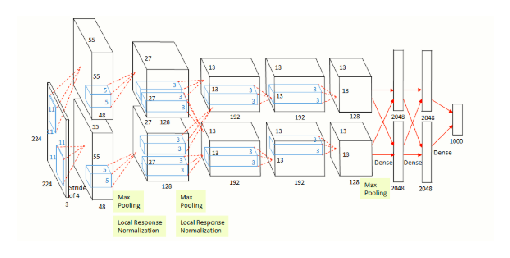
\includegraphics[width=12cm]{img/imagenet}
\caption[Alexnet]{\footnotesize{ (figura extraída de \cite{krizhevsky2012imagenet})  Imagen de la  red convolucional \textit{AlexNet}, el flujo de la información va de izquierda a derecha, con una sucesión de capas neuronales con operaciones de {\it pooling} y normalización intermedias. Aquí se puede observar claramente como varias entradas y salidas de las capas que la integran son tensores (cubos de datos).
}} 
\label{fig:imagenet}
\end{figure}      
\subsection{Desarrollo de la tesis}
Este trabajo está dividido en 6 capítulos. En este primer capítulo se da una breve introducción a los temas desarrollados, además de presentar un corto resumen de los principales resultados y conclusiones. En el próximo capítulo se introducen diferentes redes neuronales que luego serán utilizadas como referencia y darán contexto a todo lo relacionado a éstas para el resto de la tesis. En el tercer capítulo se da una recopilación similar para las descomposiciones tensoriales, dando un marco histórico de éstas y ahondando en las descomposiciones más relevantes para este trabajo.  
\par
En el cuarto capítulo se explica el rol de las descomposiciones tensoriales en \textit{deep learning}, mostrando las diferentes maneras en las cuales son utilizadas en esta área. En este capítulo también se incluye el desarrollo de la arquitectura propuesta  \textit{Tensor Ring} (TR) y los detalles de implementación para diferentes bases de datos, tanto de ésta como de la arquitectura \textit{Tensor Train} (TT) que servirá como punto de comparación. En el quinto capítulo  se muestran los resultados obtenidos para la arquitectura propuesta y las otras redes utilizadas como referencia para las diferentes bases de datos. En el último capítulo se explayan de manera más profunda las conclusiones desarrolladas en base a los resultados encontrados, además se plantean nuevas líneas de investigación que surgen a partir de lo desarrollado en este trabajo.    
\clearpage
\vspace*{0.25in}
\begin{center}
\begin{LARGE}
 \section{Capítulo \thesection: Redes Neuronales Profundas}
\end{LARGE}
\end{center}
\vspace*{0.25in}
\normalsize Este capítulo intenta dar una pequeña introducción al campo de las redes neuronales profundas. Éstas se han vuelto muy populares en los últimos años, obteniendo muy buenos resultados en diferentes aplicaciones con una gran variedad de usos en disciplinas varias. Se hace un repaso detallando las redes que serán utilizadas posteriormente en el trabajo.   
\par


\clearpage
\subsection{Introducción} \label{ssec:introduccion_redes}
Las redes neuronales profundas \textit{feedforward} \cite{goodfellow2016deep} también conocidas como \textit{multilayer perceptrons} (MLP) son uno de los modelos más conocidos de \textit{deep learning}. Su objetivo principal es el de aproximar una función $f^*$, por ejemplo un clasificador, la función  $y=f^*(\mathbf{x}) $ asigna la categoría $y$ a la entrada $\mathbf{x} \in \mathbb{R}^{N}$. Los modelos \textit{feedforward} contienen una concatenación de capas neuronales, sin realimentación, es decir, la información fluye en un solo sentido desde la entrada hacia la salida.\par 
Cada capa en una red neuronal representa una operación lineal sobre su entrada, seguida por una función no-lineal. La cantidad de capas determina la profundidad del modelo, la última capa es llamada la capa de salida mientras que las intermedias son capas ocultas. La operación realizada por las capas ocultas de una MLP puede escribirse como:
\begin{equation}
\label{Eq_MLP}
\begin{split}
\boldsymbol{h}^{(t)}&
    =   \theta^{(t)}\Big(\boldsymbol{W}^{(t)}\boldsymbol{x}^{(t-1)}+\boldsymbol{b}^{(t)}\Big) \\
\end{split}
\end{equation} \par
Siendo $\boldsymbol{h}^{(t)}\in \mathbb{R}^{I_t}$ el estado oculto de la capa $t$,  $\boldsymbol{x}^{(0)} \in \mathbb{R}^{I_0}$ la entrada de la red.
La matriz $\boldsymbol{W}^{(t)}\in \mathbb{R}^{I_t \times I_{t+1}}$ y el vector de \textit{bias} $\boldsymbol{b}^{(t)}\in \mathbb{R}^{I_{t+1}}$ constituyen los parámetros de la capa y $\theta^{(t)}$ es una función no-lineal conocida como función de activación. Entre las funciones de activación más comúnmente utilizadas se encuentran: \textit{Rectifier Linear Unit} (ReLU) \cite{nair2010rectified}, la función sigmoide y la tangente hiperbólica que se definen a continuación:
\par
\begin{equation}
\label{Eq_ReLU}
\textrm{ReLU}\ \  \theta(z) = max(z,0) 
\end{equation} \par
\begin{equation}
\label{Eq_Sig}
\textrm{Sigmoide}\ \  \theta(z) =  \frac{1}{1+\rm{e}^{-z}}
\end{equation} \par
\begin{equation}
\label{Eq_tanh}
\textrm{Tanh}\ \ \theta(z) =  \frac{\rm{e}^{2z}-1}{\rm{e}^{2z}+1}
\end{equation} \par
\par
Estas redes son llamadas \textit{neuronales} porque están inspiradas en las redes biológicas estudiadas por las Neurociencias \cite{mcculloch1943logical}. Cada capa oculta consiste en un conjunto de neuronas. Cada neurona recibe como entrada las salidas de las neuronas de la capa anterior, multiplicada por pesos sinápticos. Así, cada neurona combina todas sus entradas aplicando la función de activación (Figura \ref{fig:diagMLP}). \par
\begin{figure}[H]
 \centering
 \includegraphics[width=12cm]{img/MLP_Schema.png}
\caption[Diagrama MLP]{\footnotesize{ Una red MLP \cite{goodfellow2016deep} de profundidad $d$ que procesa la entrada \boldsymbol{$x$} y tiene salida $y$.}} 
\label{fig:diagMLP}
\end{figure}
Muchas veces a la salida de una red neuronal, se suele utilizar la función \textit{softmax} \cite{bridle1990probabilistic}. Esto convierte la salida $y\prime \in  \mathbb{R}^{k}$ de la última capa en una distribución de probabilidades, una para cada categoría ${y}_k$ a clasificar:   \par

\begin{equation}
\label{Eq_softmax}
p(y_k|\boldsymbol{x}^{(0)}) =  \frac{\rm{e}^{{y\prime}_k}}{\sum_{i=1}^{K}\rm{e}^{{y\prime}_i}} \quad \forall k \in K
\end{equation} \par
Otra ecuación utilizada es la llamada \textit{logsoftmax} que es aplicar a la función \textit{softmax} un logaritmo, la razón por la cual se utiliza es porque es numéricamente más estable \eqref{Eq_logsoftmax} (ver apéndice).\par
Uno de los elementos clave a la hora de definir cualquier algoritmo de \textit{machine learning} es la función de costo. Ésta es la encargada de definir la eficacia del algoritmo implementado, cuantifica el error entre el valor esperado y el valor de salida, permitiendo así ajustar los pesos sinápticos durante el entrenamiento de la red. Una de las funciones utilizadas para este fin es la función \textit{negative log-likelihood}, que utiliza el principio de la estimación de máxima verosimilitud de tomar como estimación de un parámetro de un evento probabilístico, aquel que da más probabilidad de que ocurra dicho evento. Dado un conjunto de N muestras con un valor esperado $\textbf{y}^{i} \in \mathbb{R}^{K}$ para cada muestra para $K$ categorías, el algoritmo tiene una salida $\textbf{y}^{i}\prime \in \mathbb{R}^{K}$, la función de costo para todo el conjunto queda definida como:   
\begin{equation}
\label{max_likelihood}
\begin{split}
\mathcal{L}= -\sum^{N}_{i}\sum^{K}_{k}y_k^i\ln{y_k^i\prime}
\end{split}
\end{equation} \par
\par
El objetivo final de la etapa de entrenamiento es reducir al mínimo el resultado de la función costo, de esa manera consiguiendo que el algoritmo se parezca lo más posible a la función original que intenta emular. Para poder lograr esto, se utilizan métodos de optimización% para minimizar el valor de esta función%
, uno de los más utilizados, es la técnica llamada \textit{gradient descent} \cite{cauchy1847methode}, basado en la idea de proveer actualizaciones en dirección opuesta al gradiente de manera que la función es minimizada en cada iteración. %que la derivada de una función nos informa hacia donde crece, lo que provee la oportunidad de reducir la función yendo en el sentido contrario del mismo. 
Para las redes neuronales \textit{feedfoward}, el algoritmo denominado \textit{back-propagation}, es el que permite que la información del costo fluya hacia atrás a través de la red, en orden para computar el gradiente. Suele confundirse como que éste es todo el algoritmo de aprendizaje para las redes neuronales \textit{feedfoward}, éste solo sirve para computar el gradiente, mientras que otros algoritmos como \textit{Stochastic Gradient Descent} (SGD) \cite{robbins1951stochastic} o Adam \cite{kingma2014adam}, son los encargados de realizar el aprendizaje  usando este gradiente.  

\subsection{Redes Neuronales Convolucionales}
\label{ssecbjetivo:CNN}
Las redes neuronales convolucionales (\textit{Convolutional Neural Networks} o CNN) son un tipo especializado de red neuronal para procesar datos con una topología similar a una cuadrícula. Fueron desarrolladas para procesar imágenes imitando el comportamiento de las redes neuronales biológicas encontradas en los mamíferos. Sin embargo, este tipo de redes tienen muchos ejemplos de aplicaciones exitosas en una gran variedad de campos, no solo en imágenes. A diferencia de una capa completamente conectada, el nombre indica que la red emplea en algunas de sus capas una operación matemática llamada convolución. Ésta es un tipo especial de operación lineal, es un operador matemático que transforma dos funciones $x$ y $w$, en una tercera función $s$, se puede denotar con un asterisco
de la siguiente manera:
\begin{equation}
\label{definicion_convolucion}
s(t)=(x*w)(t)= \sum^{\infty}_{a= -\infty} x(a)w(t-a)
\end{equation} \par
En el caso de una red neuronal, el primer argumento (la función $x$) es considerado la entrada de la red, y el segundo argumento (la función $w$) sería el núcleo o \textit{kernel}, y la salida es denominada como \textit{feature map}. Generalmente la entrada de la red es un tensor de datos, por ejemplo una imagen, y el núcleo es un tensor de parámetros que suelen ser ajustados a través de un algoritmo de aprendizaje. Dado que cada elemento de la entrada y el núcleo deben almacenarse explícitamente por separado, se puede implementar la suma infinita como una suma sobre un número finito de elementos de la matriz. Teniendo en cuenta esto se puede escribir una convolución de una imagen $\boldsymbol{I}$ de dos dimensiones con un núcleo $\boldsymbol{K}$ de la siguiente manera:
\begin{equation}
\label{definicion_convolucion_2d}
\boldsymbol{S}(t)=(\boldsymbol{I}*\boldsymbol{K})(t)= \sum_{m}\sum_{n} i_{m,n} k_{i-m,j-n} 
\end{equation} \par
Una de los principales características de una capa convolucional es que tiene interacciones dispersas, también llamada conectividad dispersa. A diferencia del caso de una capa completamente conectada, que como su nombre indica tiene todas las entradas conectadas a través de la multiplicación de una matriz de pesos a todas las salidas, la capa convolucional tiene esos pesos dispersos. Esto es el resultado de tener un \textit{kernel} más pequeño que la entrada y tiene el efecto de que éste puede extraer las características más importantes de las entradas, por ejemplo los bordes de una imagen, utilizando muchos menos parámetros y, por lo tanto, también muchas menos operaciones. \par
\begin{figure}[H]
 \centering
 \includegraphics[width=8cm]{img/convolution_example_1.PNG}
\caption[CNN interacciones dispersas]{\footnotesize{ (figura extraída de  \cite{dumoulin2016guide}) Ejemplo de una convolución de dos dimensiones sobre una matriz de 5x5 con un núcleo de tamaño 3x3.    }}
\label{fig:sparseCNN}
\end{figure}
Otra característica clave de las capas convolucional es su capacidad de compartir parámetros, esto se refiere a que se usa el mismo parámetro para más de una función en el modelo. Comparándola nuevamente con una capa completamente conectada, cada elemento de la matriz de peso es usada solamente una vez. Mientras que en el caso de una capa convolucional, los pesos están atados entre sí, porque cada valor del \textit{kernel} es usado en cada posición de la entrada. Esto también le da propiedad de ser invariante a traslaciones. 
\par
\begin{figure}[H]
 \centering
 \includegraphics[width=8cm]{img/CNN_Parameter_Sharing.png}
\caption[CNN compartir parámetros]{\footnotesize{ (figura extraída de \cite{goodfellow2016deep}) Se representa la entrada $\boldsymbol{x}$ y la salida $\boldsymbol{s}$ de una capa convolucional de núcleo de tamaño 3 (arriba) y una capa completamente conectada (abajo). En la capa convolucional se puede ver como un mismo parámetro es compartido por todas las entradas, mientras que en la capa completamente conectada, el parámetro destacado sólo se usa en una de las entradas.  }}
\label{fig:sharingCNN}
\end{figure}
Una capa de una CNN suele estar compuesta de 3 etapas. En la primer etapa, la capa convolucional aplica la operación detallada anteriormente \eqref{definicion_convolucion}. La siguiente capa suele ser una función de activación no lineal, como alguna de las funciones ya antes mencionadas, como ReLU\eqref{Eq_ReLU}, Sigmoide \eqref{Eq_Sig} o tangente hiperbólica \eqref{Eq_tanh}. La última etapa es una función de \textit{pooling}, la cual reemplaza la salida de la etapa anterior en una ubicación determinada con una
operación estadística de las salidas cercanas. Una de las operaciones es por ejemplo la función \textit{max pooling}, que reporta la salida máxima dentro de un vecindario rectangular. Otras funciones muy utilizadas son el promedio de un vecindario rectangular, la norma $L^{2}$ de un vecindario rectangular, o un promedio ponderado basado en un punto central. \par
La operación de \textit{pooling} permite que la representación se vuelva invariante a las traslaciones pequeñas en la entrada de la capa. Si hay una pequeña traslación, los valores de salida de esta etapa no deberían variar. Esto es bueno para detectar ciertas características sin darle tanta relevancia a dónde se ubica exactamente ésta.  \par
En la mayoría de las CNNs se suele agregar una capa completamente conectada, que ayuda combinar las características representadas por las salidas de la capa convolucional. Un buen ejemplo de una CNN y su arquitectura es la red \textit{AlexNet} \cite{krizhevsky2012imagenet}, que puede verse en la Figura \ref{fig:imagenet}.


\subsection{Redes Neuronales Recurrentes}
\label{ssec:RNN}
Las redes neuronales recurrentes (RNN) son una familia de redes neuronales para procesar datos secuenciales \cite{goodfellow2016deep,rumelhart1988learning}. Las secuencias de valores $\boldsymbol{X} \in \mathbb{R}^{N\times\tau}$ son de la forma $\boldsymbol{x}^{(1)},\ldots,\boldsymbol{x}^{(\tau)} \in \mathbb{R}^{\tau}$. Las RNN pueden también procesar secuencias de tamaños variables, por lo tanto $\tau$ puede no tener un valor fijo. El valor del índice $t=1..\tau$ para cualquier elemento $\boldsymbol{x}^{(t)}$ no necesariamente indica un paso en el tiempo, sino también la posición del mismo en la secuencia. Esto implica que pueden utilizarse las RNNs no solamente para eventos temporales, sino también para elementos que pueden ser separados por posición como por ejemplo una imagen, separando pedazos de la imagen por posición en la secuencia o un vídeo haciendo el caso análogo a la imagen, pero agregándole el componente del tiempo. \par 
La idea original que llevó de las redes MLPs a las RNNs es el de compartir parámetros a través de diferentes posiciones de las secuencias, lo cual permite extender y aplicar el modelo a diferentes ejemplos y poder generalizarlo. Si se tuvieran diferentes parámetros para cada valor de la secuencia, no se podrían generalizar para secuencias no vistas durante el entrenamiento. Tampoco permitiría compartir ese conocimiento a través de diferentes secuencias y a través de la repetición de diferentes elementos en distintas posiciones en el tiempo.
Las RNNs implementan ese comportamiento de compartir parámetros utilizando recursivamente la salida anterior del modelo. Esta manera de generar resultados a través de la recurrencia produce ese comportamiento.  \par
La manera en la cual las redes neuronales utilizan los bucles de la función para retener información está basado en la conectividad cíclica de las neuronas del cerebro \cite{graves2012supervised}. La ecuación con la que se puede modelar una red RNN es similar a la de un sistema dinámico \eqref{ecuacion_sistema_rnn}, que tiene un estado oculto $\boldsymbol{h}^{(t)}$ en el tiempo $t$, con una entrada $\boldsymbol{x}^{(t)}$ para el mismo tiempo y un grupo de parámetros $\boldsymbol{\theta}$ de la función $f$ que lo modela:\par
\begin{equation}
\label{ecuacion_sistema_rnn}
\boldsymbol{h}^{(t)}=f(\boldsymbol{h}^{(t-1)},\boldsymbol{x}^{(t)};\boldsymbol{\theta})
\end{equation} \par
Este procesamiento \eqref{ecuacion_sistema_rnn} puede graficarse como un diagrama de un circuito que funciona en tiempo real, que se alimenta de una entrada y una retroalimentación por cada instante de tiempo (Figura \ref{fig:diagRNN}). Cada nodo representa un paso en el tiempo donde, en cada momento, es calculado el estado oculto. Esto permite ver que se puede procesar la entrada sin importar el largo de la secuencia y es posible usar la misma función $f$ para cada paso.     \par
\begin{figure}[H]
 \centering
 \includegraphics[width=15cm]{img/RNN_Schema.png}
\caption[Diagrama RNN]{\footnotesize{ Una red recurrente que procesa la entrada \boldsymbol{$x$} y el estado actual \boldsymbol{$h$} a través del tiempo \eqref{ecuacion_sistema_rnn}.}}
\label{fig:diagRNN}
\end{figure}
\subsection{Vanilla RNN}
\label{ssec:vanillaRNN}

A la red RNN más difundida le atribuiremos el nombre de \textit{Vanilla RNN}. La arquitectura que se referencia para todas las redes es la de una red recurrente que tiene como entrada una secuencia entera y produce una única salida (Figura \ref{fig:RNN_single_output}).

\begin{figure}[H]
 \centering
 \includegraphics[width=12cm]{img/RNN_Schema_Single_Output.png}
\caption[Diagrama RNN con una sola salida]{\footnotesize{ Una red recurrente \cite{goodfellow2016deep} \textit{unfolded} con una sola salida al final de la secuencia.  }}
\label{fig:RNN_single_output}
\end{figure}
El cálculo de los valores de salida \boldsymbol{$o$} de la red se realiza utilizando  \textit{forward propagation}. Si se observa la Figura \ref{fig:RNN_single_output}, se puede ver cómo se calcula utilizando un conjunto de parámetros de la red. 

También se puede usar una red que tenga una salida por paso de tiempo (Figura \ref{fig:RNN_multiple_outputs}). Este tipo de red se conoce como \textit{Elman network} \cite{elman1990finding}. Otra variación interesante con la que se puede experimentar, es cambiar la recurrencia y, en vez de realimentar el estado con el anterior, se puede utilizar la salida anterior (Figura \ref{fig:RNN_multiple_outputs_differente_recurrency}). Este tipo de red se conoce como \textit{Jordan network} \cite{jordan1997serial}.  \par

Las ecuaciones que se usan para el cálculo de la salidas para cada paso del tiempo, para el caso de la \textit{Elman Network} \cite{elman1990finding} (Figura \ref{fig:RNN_multiple_outputs}), son las siguientes:
\begin{equation}
\label{eq_rnn_vanilla_h}
\boldsymbol{h}^{(t)}=\theta(\boldsymbol{U}\boldsymbol{x}^{(t)}+\boldsymbol{W}\boldsymbol{h}^{(t-1)} +\boldsymbol{b}^h)
\end{equation} \par
\begin{equation}
\label{eq_rnn_vanilla_o}
\boldsymbol{o}^{(t)}=\boldsymbol{V}\boldsymbol{h}^{(t)}+\boldsymbol{b}^o
\end{equation} \par
\begin{equation}
\label{eq_rnn_vanilla_y}
\boldsymbol{\hat{y}}^{(t)}=softmax(\boldsymbol{o}^{(t)})
\end{equation} \par
 Los parámetros que se utilizan en las ecuaciones, los vectores de bias $\textbf{b}^H$ y $\boldsymbol{b}^o$, y las matrices $\boldsymbol{U}$, $\boldsymbol{W}$ y $\boldsymbol{V}$, además del estado inicial $\boldsymbol{h}^{(0)}$, son los que luego serán ajustados con el proceso de \textit{backpropagation} de la red. La Figura \ref{fig:RNN_cell} muestra la representación gráfica de una celda en una red RNN. 
\begin{figure}[H]
 \centering
 \includegraphics[width=10cm]{img/RNN_Cell_Schema.png}
\caption[Diagrama Celda RNN]{\footnotesize{ Una celda de una red RNN, donde se puede ver el procesamiento de un paso de la secuencia.  }}
\label{fig:RNN_cell}
\end{figure}
 
 \par 
 Se puede calcular una salida por paso, y en el caso de la red con una sola salida (Figura \ref{fig:RNN_single_output}) solamente es necesario calcular ésta para el último paso de la red, donde $t=\tau$. Para el caso de una \textit{Jordan Network} (Figura \ref{fig:RNN_multiple_outputs_differente_recurrency}), la única ecuación a modificar es la que calcula el estado oculto $\boldsymbol{h}^{(t)}$ \eqref{eq_rnn_vanilla_h}. El concepto detrás de este cambio es que, si cada salida es una acción, esto permite a la red recordar las acciones realizadas y que éstas sean tomadas en cuenta a la hora de tomar la próxima acción. Esto puede ser aplicado en varias tareas, como por ejemplo a la hora de traducir una oración entre lenguajes naturales \cite{sutskever2014sequence}, donde es importante tener como entrada la salida anterior, que en ese caso será una secuencia de texto. La ecuación se modifica utilizando como entrada en vez del estado oculto anterior $\boldsymbol{h}^{(t-1)}$, la salida anterior $\boldsymbol{o}^{(t-1)}$ : \par
 \begin{equation}
\label{eq_jordan_rnn_vanilla_h}
\boldsymbol{h}^{(t)}=\theta\Big(\boldsymbol{U}\boldsymbol{x}^{(t)}+\boldsymbol{W}\boldsymbol{o}^{(t-1)} + \boldsymbol{b}^h\Big)
\end{equation} \par
 Cada uno de los parámetros se encuentra asociado a una de tres transformaciones de una red RNN, de la entrada a un estado oculto ($\boldsymbol{U}$), de un estado oculto al próximo estado oculto ($\boldsymbol{W}$) y de un estado oculto a la salida ($\boldsymbol{V}$). Cada uno de ellos puede estar asociado a una transformación que podemos llamar \textit{shallow}, que es una trasformación posible en una capa de una red MLP \eqref{Eq_MLP}.
\begin{figure}[H]
 \centering
 \includegraphics[width=13cm]{img/RNN_Schema_Multiple_Output.png}
\caption[Diagrama RNN  \textit{Elman network}]{\footnotesize{ Una red recurrente \cite{goodfellow2016deep} \textit{unfolded} conocida como \textit{Elman network} \cite{elman1990finding}.  }}
\label{fig:RNN_multiple_outputs}
\end{figure}
\begin{figure}[H]
 \centering
 \includegraphics[width=13cm]{img/RNN_Schema_Multiple_Output_Different_Recurrency.png}
\caption[Diagrama RNN  \textit{Jordan network}]{\footnotesize{ Una red recurrente \cite{goodfellow2016deep} \textit{unfolded} conocida como \textit{Jordan network} \cite{jordan1997serial}.  }}
\label{fig:RNN_multiple_outputs_differente_recurrency}
\end{figure}
Existen dos problemas ampliamente conocidos a la hora de entrenar redes RNN, los cuales son denominados : \textit{exploding gradient problem} \cite{hochreiter1991untersuchungen,bengio1993problem,hochreiter2001gradient} y
\textit{vanishing gradient problem}. El \textit{exploding gradient problem} se refiere a un gran incremento en la norma del gradiente durante el entrenamiento, causado por la explosión de los componentes de largo plazo. Esto puede resultar en inestabilidad en el proceso de aprendizaje. Análogamente, \textit{vanishing gradient problem} se refiere al comportamiento opuesto, donde el componente de largo plazo converge exponencialmente a una norma cero, volviendo imposible que la red aprenda correlaciones, entre eventos distantes temporalmente, eliminando una de las ventajas de este tipo de redes. Esto refleja de alguna manera una contrapartida entre el aprendizaje por \textit{gradient descent} y la capacidad de poder capturar dependencias a medida que la duración de las mismas aumentan a través del tiempo. Este problema no se presenta únicamente en las redes RNN pero, debido a la profundidad de este tipo de redes y la forma en la cual funciona su algoritmo de feedfoward, son unas de las mas afectadas por este fenómeno. 
\par
Una de las variantes para aliviar este problema es la de usar una función de activación ReLU \eqref{Eq_ReLU}\cite{xu2015empirical,glorot2011deep}, debido a la forma que toma la salida, el gradiente de la función ReLU sólo puede tomar como valores 0 o 1, evitando la saturación y por lo tanto el efecto de desvanecimiento o explosión. Otras maneras de solucionar este problema, además de modificar la función de activación, es utilizar otros tipos de redes recurrentes como la red LSTM \cite{hochreiter1997long} (ver Apéndice, sección \ref{ssec:LSTM}) o la red GRU \cite{cho2014learning} (ver Apéndice, sección \ref{ssec:GRU}) o hacer \textit{gradient clipping} \cite{pascanu2013difficulty}, limitando el crecimiento del gradiente. Una alternativa, que también es muy utilizada, es modificar la inicialización de los parámetros. Ésta es un área muy investigada, ya que, en la práctica, se notó que afecta al rendimiento de la red de manera considerable. Se demostró que inicializar los valores de la red como una matriz identidad es una técnica efectiva para combatir el problema de los gradientes que desaparecen, y las redes así inicializadas se las llama IRNN (identity RNN) \cite{le2015simple}.Otros métodos conocidos de inicialización son la \textit{xavier initialization} \cite{glorot2010understanding} o la \textit{kaiming initialization} \cite{he2015delving}.
\par
 \clearpage
\vspace*{0.25in}
\begin{center}
\begin{LARGE}
 \section{Capítulo \thesection: Descomposiciones tensoriales}
\end{LARGE}
\end{center}
\vspace*{0.25in}
\normalsize Este capítulo se enfoca en las descomposiciones tensoriales, con una introducción teórica a los tensores, donde se especifican tanto la notación como las operaciones que se utilizan a lo largo del trabajo. Luego se hace un repaso histórico de las descomposiciones tensoriales y sus aplicaciones actuales en diferentes campos. También se explican en detalle dos descomposiciones que, más adelante en el trabajo, serán aplicadas en redes neuronales profundas: Tensor Ring (TR) y Tensor Train (TT). 
\par





\clearpage
 
 
Un tensor es la generalización multidimensional de un vector o matriz \cite{kolda2009tensor}. Este término generalmente se utiliza para referirse a un arreglo que tiene tres o más índices (tensores de orden alto), pero también puede usarse para describir una matriz (orden 2), un vector (orden 1), o un escalar (orden 0). El uso de tensores es común en varias áreas, pero no debe ser confundido por los usados en campos como la física y la ingeniería, comúnmente llamados \textit{campos tensoriales}. Un subtensor es una parte del tensor original que se obtiene fijando un subconjunto de índices.
\par
Los subtensores de orden 1, que son vectores llamados \textit{fibers}, se obtienen fijando todos menos un índice, mientras que los tensores de orden 2 son matrices llamados \textit{slices}, y se obtienen fijando todos los índices menos dos. Los tensores denominados simples son aquellos tensores que pueden ser escritos como un producto de tensores de orden 1:
\begin{equation}
\label{eq_simple}
\mathcal{X}= \boldsymbol{b}_{r}^{(1)} \otimes	 \boldsymbol{b}_{r}^{(2)} \otimes	  \ldots  \otimes	 \boldsymbol{b}_{r}^{(N)}   
\end{equation}
Los tensores tienen, asimismo, un rango que se define como la cantidad mínima necesaria de tensores simples (también denominados de rango 1) que sumados dan como resultado dicho tensor.    
\begin{figure}[H]
 \centering
 \includegraphics[width=9cm]{img/ejemplo_tensor_fiber_3d.png}
\caption[Ejemplo \textit{fiber} en un tensor]{\footnotesize{ Ejemplo de un tensor $\mathcal{G}^{(k)} \in \mathbb{R}^{R_k \times N_k \times R_{k+1}}$ de orden 3, con una \textit{fiber} $\boldsymbol{g}^{(k)}(r_k,r_{k+1})$.}}

\label{fig:fiber_in_tensor}
\end{figure}\par
\begin{figure}[H]
 \centering
 \includegraphics[width=7cm]{img/ejemplo_tensor_slice_3d.png}
\caption[Ejemplo \textit{slice} en un tensor]{\footnotesize{ Ejemplo de un tensor $\mathcal{G}^{(k)} \in \mathbb{R}^{R_k \times N_k \times R_{k+1}}$ de orden 3, con una \textit{slice} $\boldsymbol{G}^{(k)}(n_k)$.}}
\label{fig:slice_in_tensor}
\end{figure}\par
\subsection{Notación de Tensores}
 \FloatBarrier
\begin{table*}[hbt!]
\centering
\begin{tabular}{p{0.4\linewidth}p{0.5\linewidth}}
\hline
\multicolumn{2}{c}{\large  Notación básica } \\
\hline 
 \large $\mathcal{A}, \textbf{A}, \textbf{a}, a$  & 
 \large Tensor, Matriz, Vector, Escalar \\ 
 
  \large $\mathcal{D}= diag_N(\lambda_1,\lambda_2 \ldots,\lambda_N)$  & 
 \large Tensor diagonal de orden N \\ 
 
   \large $\textbf{D}= diag_N(\lambda_1,\lambda_2\ldots,\lambda_N)$  & 
 \large Matriz diagonal de orden N \\ 
 
\large $\textbf{B}^{(i)}$ & 
\large Matriz factor i \\

\large $\textbf{b}^{(i)}_{j}$ & 
\large Vector columna j de la matriz
 $\textbf{B}^{(i)}$\\

 \large $a_{r1r2 \ldots rN}$&
 \large Elemento de un  tensor $\mathcal{A} \in \mathbb{R} ^{R_1 \times R_2 \times \ldots \times R_N}$\\
 
\large $\mathcal{G}^{(i)}$ & 
\large Tensor núcleo número $i$ de orden 3 con índices $j$,$k$,$l$ para cada uno de sus dimensiones \\

\large $\textbf{G}^{(i)}(j)$ &
\large \textit{Slice} de un Tensor Núcleo $\mathcal{G}^{(i)}$ de orden 3 con el índice $j$ fijado \\
\large $\textbf{g}^{(i)}(j,k)$ & 
\large \textit{Fiber} de un Tensor Núcleo $\mathcal{G}^{(i)}$ de orden 3 con los índices $j$ y $k$ fijados \\
\large  $\textbf{A}^{T}, \textbf{a}^{T}$ &
\large   Matriz transpuesta, Vector transpuesto\\
 

\hline\hline 
\end{tabular}
\label{table:NotacionBasica}
\caption{Notación básica de Tensores}
\end{table*}
 \FloatBarrier

\begin{table*}[ht]
\centering
\begin{tabular}{p{0.35\linewidth}p{0.65\linewidth}}
\hline
\multicolumn{2}{c}{\large  Notación de operaciones } \\
\hline 
 \large  $\mathcal{C}= \mathcal{A} \times_n \boldsymbol{B}$ & 
 \large  Producto modo$-n$ de $\mathcal{A} \in$ $\mathbb{R} ^{I_1 \times I_2 \times \ldots \times I_N}$ y 
 \large  $\boldsymbol{B} \in$ $\mathbb{R}^{J_n \times I_n}$ siendo $\mathcal{C} \in$ $\mathbb{R} ^{I_1 \times I_2 \times \ldots \times I_{n-1} \times J_n \times I_{n+1} \times \ldots \times I_N}$ con $C_{i_1 \ldots i_{n-1}j_ni_{n+1} \ldots i_N}$ $=\sum_{i_n=1}^{I_n} a_{i_1 \ldots i_{n-1}i_ni_{n+1} \ldots i_N} \cdot b_{j_n i_n} $\\
 
 \large  $\mathcal{C}= \Vert \mathcal{A};\boldsymbol{B}^{(1)},\boldsymbol{B}^{(2)} \ldots \boldsymbol{B}^{(N)} \Vert $ & 
 \large  Producto multilineal completo $\mathcal{C}= \mathcal{A} \times_1 \boldsymbol{B}^{(1)} \times_2 \boldsymbol{B}^{(2)}  \ldots  \times_N \boldsymbol{B}^{(N)}$ \\
 
 \large $\mathcal{C} =\mathcal{A} \otimes	 \mathcal{B}$ & 
 \large Producto exterior de $\mathcal{A} \in \mathbb{R} ^{I_1 \times I_2 \times \ldots  \times I_N}$ y $\mathcal{B} \in \mathbb{R} ^{J_1 \times J_2 \times \ldots  \times J_M}$ siendo $\mathcal{C} \in \mathbb{R} ^{I_1 \times I_2 \times \ldots  \times I_N \times J_1 \times J_2 \times \ldots  \times J_M}$ con $c_{i_1i_2 \ldots i_Nj_1j_2 \ldots j_M} = a_{i_1i_2 \ldots i_N} \cdot b_{j_1j_2 \ldots j_M} $\\
 
  \large $\mathcal{C} =\mathcal{A} \circ	 \mathcal{B}$ & 
 \large Producto Hadamard de $\mathcal{A} \in \mathbb{R} ^{I_1 \times I_2 \times \ldots  \times I_N}$ y $\mathcal{B} \in \mathbb{R} ^{I_1 \times I_2 \times \ldots  \times I_N}$ siendo $\mathcal{C} \in \mathbb{R} ^{I_1 \times I_2 \times \ldots  \times I_N}$ con $c_{i_1i_2 \ldots i_N} = a_{i_1i_2 \ldots i_N} \cdot b_{i_1i_2 \ldots i_N} $\\

 \large $c =  \langle \mathcal{A},\mathcal{B} \rangle$ & 
 \large Producto escalar de $\mathcal{A} \in \mathbb{R} ^{I_1 \times I_2 \times \ldots  \times I_N}$ y $\mathcal{B} \in \mathbb{R} ^{I_1 \times I_2 \times \ldots  \times I_N}$ siendo c un escalar con $c = \sum_{i_1=1}^{I_1} \sum_{i_2=1}^{I_2} \dots  \sum_{i_N=1}^{I_N} a_{i_1i_2 \ldots i_N} \cdot b_{i_1i_2 \ldots i_N} $\\
 
 \large $\mathrm{Tr}(\textbf{A})= \sum^N_{n=1}a_{nn}$&
 \large Traza de una matriz $\textbf{A} \in \mathbb{R} ^{N \times N}$ es la suma de los elementos en sus diagonales \\
 
\hline\hline 
\end{tabular}
\caption{Notación de operaciones de Tensores}
\label{table:NotacionOperaciones}
\end{table*}

\subsubsection{Notación de Diagrama de Tensores}
Hay varios sistemas de notación gráfica utilizados para tensores y redes de los mismos. En este documento se utilizarán las siguientes convenciones \cite{tensornetwork.org}:
\begin{itemize}
\item Un tensor es notado como un círculo sólido y sus índices son las líneas que emanan de éste (Figura \ref{fig:ejemplo_notacion}). 
\item Una línea que conecta dos implica una contracción o suma sobre los índices conectados (Figura \ref{fig:ejemplo_contraccion}). 
\end{itemize}
\begin{figure}[H]
 \centering
 \includegraphics[width=12cm]{img/ejemplos_tensores.png}
\caption[Ejemplos notación de diagrama de tensores]{\footnotesize{ Ejemplos de la notación de diagrama de tensores para un tensor \textbf{v} de orden 1 (vector), un tensor \textbf{M} de orden 2 (matriz) y un tensor \textbf{$\mathcal{T}$} de orden 3. Además se nota un escalar como un cuadrado.}} 
\label{fig:ejemplo_notacion}
\end{figure}
\begin{figure}[H]
 \centering
 \includegraphics[width=10cm]{img/ejemplo_contracciones_tensores.png}
\caption[Ejemplos notación de diferentes contracciones]{\footnotesize{Ejemplos de notación de diferentes contracciones. El primer ejemplo es el producto de una matriz por un vector, el siguiente es el de una matriz por otra matriz y el tercero es la traza del producto. }} 
\label{fig:ejemplo_contraccion}
\end{figure}

\subsection{Historia}
Fue Hitchcock en 1927 \cite{hitchcock1927expression,hitchcock1928multiple} quien primero introdujo la idea de descomponer tensores, demostrando que se pueden representar a través de un conjunto de tensores o vectores de menor orden. Hitchcock propuso descomponer un tensor como la suma de un producto de vectores. Esto más los aportes de Catell en 1952 \cite{cattell1952three}, fueron la inspiración para que en los años 70s se desarrollaran las descomposiciones CANDECOMP (Descomposición canónica) \cite{carroll1970analysis} y PARAFAC \cite{harshman1970foundations}. Éstas son la base de una de las descomposiciones más conocidas y estudiadas, la CANDECOMP/PARAFAC \cite{kiers2000towards}, también llamada la descomposición poliádica canónica (CPD) o tensor de Kruskal (Figura \ref{fig:descomposicion_cpd}). La CPD es utilizada para hacer procesamiento y análisis de señales, o en análisis exploratorio de datos. La CPD representa un tensor $\mathcal{X} \in \mathbb{R} ^{I_1 \times I_2 \times \ldots  \times I_N}$ de orden N como una combinación lineal de tensores de rango 1: \par
\begin{equation}
\label{eq_descomposicion_cpd}
\mathcal{X}= \sum_{r=1}^{R} \lambda_{r} \cdot (\boldsymbol{b}_{r}^{(1)} \otimes	 \boldsymbol{b}_{r}^{(2)} \otimes	  \ldots  \otimes	 \boldsymbol{b}_{r}^{(N)})     
\end{equation}
Esta ecuación también se puede escribir como un producto multilineal con un núcleo diagonal $\mathcal{D} = diag_N(\lambda_1,\lambda_2,..,\lambda_R)$: 
\begin{equation}
\label{eq_producto_multilineal_CPD}
 \begin{split} 
\mathcal{X}&
=\mathcal{D} \times_1 \boldsymbol{B}^{(1)} \times_2 \boldsymbol{B}^{(2)}  \ldots  \times_N \boldsymbol{B}^{(N)} \\
&=\Vert \mathcal{D};\boldsymbol{B}^{(1)},\boldsymbol{B}^{(2)} \ldots ,\boldsymbol{B}^{(N)} \Vert 
\end{split}
\end{equation}
Kruskal en 1977 \cite{kruskal1977three} propuso el concepto de rango de un tensor, análogo al rango de una matriz, que se define como la menor cantidad de tensores de rango 1 (tensores que son producto de vectores) que sumados dan ese mismo tensor. Notablemente, hallar el rango de un tensor, también llamado rango canónico, es NP-Hard \cite{haastad1990tensor}, inclusive para un tensor de orden 3. Esto, junto a la dificultad de encontrar una buena aproximación de tensores de bajo rango, inclusive cuando es sabido que éste existe, suele disuadir el uso de este formato. Por dicha razón también se incentivó el uso de otros modelos de descomposición, a pesar de tener más parámetros que la canónica, ya que son más fáciles de lidiar numéricamente. Aún así es importante notar la baja cantidad de parámetros del modelo CPD $\mathcal{O}(dnr)$, siendo $d$ el orden del tensor, $n$ el tamaño de cada uno de los vectores y $r$ el rango.  \par
\begin{figure}[ht]
 \centering
 \includegraphics[width=10cm]{img/descomposicion_canonica.png}
\caption[Ejemplo descomposición CPD]{\footnotesize{Ejemplo de una descomposición CPD de un tensor  \boldsymbol{$\mathcal{X}$} de orden 3 de dimensiones IxJxK, en el producto de 3 matrices, \textbf{A} (IxR),\textbf{B} (IxR) y \textbf{C} (KxR) por el tensor diagonal \boldsymbol{$\mathcal{G}$} también de orden 3 (RxRxR).
}} 
\label{fig:descomposicion_cpd}
\end{figure}

Las descomposiciones tensoriales volvieron a popularizarse debido a su utilidad a la hora de realizar análisis de datos, sobre todo con grandes volúmenes de datos (big data), que son representados de manera multidimensional. Es una más de las herramientas que se utilizan a la hora de tratar de resolver la maldición de la dimensionalidad (\textit{curse of dimensionality}) \cite{bellman2015adaptive}. Los datos a analizar pueden venir naturalmente en forma de un tensor, como por ejemplo, una imagen o un vídeo, o pueden ser datos representados en formatos más simples, como un vector o una matriz, tensorizados con el fin de poder organizarlos de manera más simple o de poder darle más sentido a su representación, como por ejemplo, las mediciones de un grupo de sensores a través del tiempo o respecto de sus canales. \par
Las descomposiciones proveen la capacidad de realizar separación ciega de fuentes (BSS), es decir, separar señales de diferentes fuentes provenientes de varios sensores. Éstas también son capaces de realizar reducción de dimensionalidad y lidiar datos con valores faltantes o ruidosos. Son una buena herramienta para analizar la relación e interacción entre diferentes dimensiones o modos de los datas, pudiendo las redes tensoriales tomar múltiples formas que pueden adaptarse dependiendo de su naturaleza. Otra aplicación que será mencionada más adelante es su poderosa capacidad de compresión, pasando de datos multidimensionales a una factorización en matrices o tensores de muy bajo rango y orden. Esto también permite que sea más fácil y menos costoso realizar ciertas operaciones matemáticas, que al mismo tiempo, debido a la forma de las redes, se vuelven más fácil de interpretar. \par

La descomposición de Tucker, introducida en 1963 \cite{tucker1963implications}, consiste en un tensor núcleo pequeño que es multiplicado por matrices (factores) en cada dimensión (Figura \ref{fig:descomposicion_tucker}). Suele ser usada para el análisis de componentes principales (PCA) de orden alto. El problema de éste tipo de descomposición es que la cantidad de parámetros que requiere son $\mathcal{O}(dnr+r^d)$, teniendo un término exponencial que, para un tensor de orden grande, se vuelve prohibitivo. Esta descomposición funciona para dimensiones chicas, especialmente para el caso de un tensor con 3 dimensiones \cite{oseledets2008tucker}. Además de su uso como PCA,  tiene otros usos interesantes como en \textit{computer vision} \cite{vasilescu2002multilinear}, o en el reconocimiento de dígitos manuscritos \cite{savas2007handwritten}. 
\par
La descomposición de Tucker representa un tensor $\mathcal{X} \in \mathbb{R} ^{I_1 \times I_2 \times \ldots \times I_N}$ de orden N  como una transformación multilineal de un tensor núcleo $\mathcal{G} \in \mathbb{R} ^{R_1 \times R_2 \times \ldots \times R_N}$ más denso y pequeño del original multiplicado por matrices $\boldsymbol{B}^{(n)}=[\boldsymbol{b}^{(1)},\boldsymbol{b}^{(2)}, \ldots ,\boldsymbol{b}^{(n)}] \in \mathbb{R} ^{I_n \times R_n}$, $n = 1,2, \ldots ,N$, dado por:   \par
\begin{equation}
\mathcal{X}= \sum_{r_1=1}^{R_1}\sum_{r_2=1}^{R_2} \dots \sum_{r_N=1}^{R_N} g_{r1r2 \ldots rN} \cdot \Big(\boldsymbol{b}_{r_1}^{(1)} \otimes	 \boldsymbol{b}_{r_2}^{(2)} \otimes	  \ldots \otimes	 \boldsymbol{b}_{r_n}^{(N)}\Big),     
\end{equation}
o equivalentemente:
\begin{equation}
\label{producto_multilineal_tucker}
 \begin{split}
\mathcal{X}&
=\mathcal{G} \times_1 \boldsymbol{B}^{(1)} \times_2 \boldsymbol{B}^{(2)}  \ldots \times_N \boldsymbol{B}^{(N)} \\
&=\Big \Vert \mathcal{G};\boldsymbol{B}^{(1)},\boldsymbol{B}^{(2)} \ldots ,\boldsymbol{B}^{(N)} \Big  \Vert 
\end{split}
\end{equation}
En la representación de la descomposición de Tucker como un producto multilineal \eqref{producto_multilineal_tucker} comparándola con la representación de la CPD \eqref{eq_producto_multilineal_CPD}, podemos ver que la última es un caso especial de la anterior, es decir con un  tensor núcleo $\mathcal{G}$  diagonal y con todas sus dimensiones iguales. 
 \begin{figure}[H]
 \centering
 \includegraphics[width=10cm]{img/descomposicion_tucker.png}
\caption[Ejemplo descomposición de Tucker]{\footnotesize{Ejemplo de una descomposición de Tucker de un tensor  \boldsymbol{$\mathcal{X}$} de orden 3 de dimensiones IxJxK, en el producto de 3 matrices, \textbf{A} (IxP),\textbf{B} (IxQ) y \textbf{C} (KxR) por el tensor \boldsymbol{$\mathcal{G}$} también de orden 3 (PxQxR). Es importante notar que a diferencia de CPD, donde el núcleo es diagonal, en Tucker es denso.
}} 
\label{fig:descomposicion_tucker}
\end{figure}
De la descomposición de Tucker surge otra llamada Hierarchical Tucker (HT), desarrollada por Hackbusch \textit{et al.}. \cite{hackbusch2009new}, que realiza el mismo proceso, pero de manera jerárquica, lo que lo vuelve más complejo y compacto. Este tipo de descomposiciones, donde el número de tensores y matrices involucrados en la descomposición es grande, se conoce como Redes Tensoriales ({\it Tensor Networks}) y pueden representarse sintéticamente a través de diagramas de redes. Por ejemplo, la Figura \ref{fig:descomposicion_ht} muestra la red asociada a una descomposición HT.\par

\begin{figure}[H]
 \centering
 \includegraphics[width=10cm]{img/descomposicion_hierarchical_tucker.png}
\caption[Ejemplo descomposición Jerárquica de Tucker]{\footnotesize{Ejemplo de una descomposición HT de un tensor  \boldsymbol{$\mathcal{X}$} de orden 8.
}} 
\label{fig:descomposicion_ht}
\end{figure}
\subsection{Tensor Train}
\textit{Tensor Train} (TT) \cite{oseledets2011tensor} es otra red tensorial que puede ser interpretada como un HT, en el cual todos los nodos están conectados en cascada, haciéndolo un tren de núcleos (Figura \ref{fig:descomposicion_tt}), de ahí su nombre. Tanto en el caso de TT como el de HT tienen como ventaja que la representación de un tensor de orden alto está reducida a un conjunto $d$ de tensores de orden 2 y 3, y por lo tanto están libres de la maldición de la dimensionalidad. El costo de almacenamiento de la descomposición de TT es de $\mathcal{O}(dnr^2)$. Los dimensiones de entrada y salida de los tensores núcleos son llamados  \textit{TT-Ranks} o \textit{rangos} de la descomposición. Éstos solamente tienen como valores restringidos el rango de entrada del primer tensor y el último rango de salida del último tensor, $r_1=r_{d+1}=1$, haciendo que esos tensores sean matrices, $\mathcal{G}^{(1)} \in \mathbb{R} ^{1 \times I_1 \times R_2 }$ y $\mathcal{G}^{(N)} \in \mathbb{R} ^{R_N \times I_N \times 1}$. Los otros rangos no están necesariamente restringidos, pero generalmente es común que los rangos de los tensores intermedios sean más grandes que aquellos de los extremos.  
\par
La descomposición TT está basada en aproximar cada elemento del tensor por un producto secuencial de matrices, donde la primera y la última matriz son vectores, para asegurarse que el resultado sea escalar. Esta descomposición es muy utilizada en la física, es conocida como MPS (\textit{matrix product state}). Siendo un elemento $x_{i_1,i_2, \ldots ,i_N}$ del tensor $\mathcal{X} \in \mathbb{R}^{I_1 \times I_2 \times  \ldots \times I_N}$ , es el producto secuencial de unas matrices de la forma $\boldsymbol{G}^{(n)}(i_n)\in \mathbb{R} ^{R_{n-1} \times R_n } $,  una \textit{slice} de un núcleo $\mathcal{G}^{(n)}$ $\forall$ $n=1 \ldots N$: 
\par
\begin{equation}
\label{slice_representation_TT}
x_{i_1,i_2, \ldots ,i_N}= \boldsymbol{G}^{(1)}(i_1) \boldsymbol{G}^{(2)}(i_2) \ldots \boldsymbol{G}^{(N)}(i_N)  
\end{equation} \par
Teniendo en cuenta que ${G}^{(1)}(i_1)\in \mathbb{R} ^{1 \times R_2 }$ y ${G}^{(N)}(i_N)\in \mathbb{R} ^{R_N \times 1 }$y $g_{r_n,i_n,r_{n+1}}^{(n)}$ un elemento del tensor $\mathcal{G}^{(n)}$puede escribirse como: \par
\begin{equation}
\label{slice_representation_TT_with_vectos}
\begin{split}
x_{i_1,i_2, \ldots ,i_N}
&=\sum^{R_1}_{r_1=1}\sum^{R_2}_{r_2=1}\dots\sum^{R_N}_{r_N=1}g_{1,i_1,r_2}^{(1)} \cdot g_{r_2,i_2,r_3}^{(2)} \ldots g_{r_N,i_N,1}^{(N)}
\end{split}
\end{equation} \par
\begin{figure}[H]
 \centering
 \includegraphics[width=14cm]{img/descomposicion_tensor_train.png}
\caption[Ejemplo descomposición \textit{Tensor Train}]{\footnotesize{Ejemplo de una descomposición \textit{Tensor Train} de un tensor \boldsymbol{$\mathcal{X}$} de orden 4.  
}} 
\label{fig:descomposicion_tt}
\end{figure}
\subsection{Tensor Ring}
\label{ssec:tensor_ring}
En la actualidad se siguen desarrollando nuevos tipos de descomposiciones como \textit{Tensor Ring} (TR) \cite{zhao2016tensor} (Figura \ref{fig:descomposicion_tr}), que fue pensada con el propósito de reducir el tamaño de almacenamiento necesario para guardar tensores de alta dimensionalidad. Está basada en TT, con un cambio en la conexión de los  núcleos, el primero está conectado con el último, formando justamente un anillo de tensores núcleos. Esto ataca una de las restricciones más importantes de la descomposición TT, los valores de los rangos fijos, $r_1=r_{d+1}=1$, pudiendo llevar a limitar la capacidad y flexibilidad de la descomposición. Para atacar ésta y otras restricciones como los patrones de los rangos y el orden específico en el cual se debe realizar el producto multilineal, surgió esta nueva descomposición.  \par
 De la misma manera que en la descomposición TT, en este caso los valores de las dimensiones exteriores del tensor $R_n$ $\forall$ $n=1 \ldots N$ son llamados \textit{TR-Ranks} o \textit{rangos} de la descomposición. El principal cambio propuesto es sacar las restricciones de los rangos de tamaño fijo en el primer y último tensor. Debido a que estos rangos pasan a tener valores distintos de uno, se utiliza la traza para reducir la matriz generada al valor de un elemento del tensor. Finalmente, para expresar un elemento del tensor $t_{i_1,i_2, \ldots ,i_N}$ de un tensor $\mathcal{T} \in \mathbb{R} ^{I_1 \times I_2 \times \ldots \times I_N}$, se utiliza la traza del producto secuencial de unas matrices de la forma $\boldsymbol{G}^{(n)}(i_n)\in \mathbb{R} ^{R_{n-1} \times R_n } $ una \textit{slice} de un núcleo $\mathcal{G}^{(n)} \in \mathbb{R} ^{R_{n-1}\times I_n \times R_n }$  $\forall$ $n=1 \ldots N$:  \par
\begin{equation}
\label{slice_representation_TR}
\begin{split}
t_{i_1,i_2, \ldots ,i_N}&
= \mathrm{Tr} \Big\{\boldsymbol{G}^{(1)}(i_1) \boldsymbol{G}^{(2)}(i_2) \ldots \boldsymbol{G}^{(N)}(i_N) \Big\}   \\
      &= \mathrm{Tr} \Bigg\{\prod_{k=1}^{N}\boldsymbol{G}^{(k)}(i_k) \Bigg\} 
\end{split}
\end{equation} \par
Es importante que cada par de tensores núcleos compartan una dimensión, siendo $\mathcal{G}^{(n)} \in \mathbb{R} ^{R_{n-1}\times I_n \times R_n }$ y $\mathcal{G}^{(n+1)} \in \mathbb{R} ^{R_{n}\times I_n \times R_{n+1} }$ $\forall$ $n=1 \ldots N$, lo cual genera que para el tensor $N$, $R_1=R_{N+1}$. Esto asegura que el producto del producto secuencial sea una matriz cuadrada, por lo tanto pueda aplicarse la traza de la misma.
Una propiedad importante que tiene esta descomposición a diferencia de la TT es que se pueden permutar los tensores núcleos sin cambiar el resultado final. Haciendo un desplazamiento circular de las dimensiones de un tensor  $\mathcal{T} \in \mathbb{R} ^{I_1 \times I_2 \times \ldots \times I_N}$ de una descomposición dada por $\mathcal{T}=\mathfrak{R}(\mathcal{G}^{(1)},\mathcal{G}^{(2)}, \ldots ,\mathcal{G}^{(N)})$ por $k$ entonces se tiene una descomposición $ \overleftarrow{\mathcal{T}}^k$ que es igual a la original. Tomando en cuenta \eqref{slice_representation_TR} se puede escribir:\par 
\begin{equation}
\label{TR_shift_theorem}
\begin{split}
t_{i_1,i_2, \ldots ,i_N}&
= \mathrm{Tr} \Big\{\boldsymbol{G}^{(2)}(i_2)\boldsymbol{G}^{(3)}(i_3) \ldots \boldsymbol{G}^{(N)}(i_N),\boldsymbol{G}^{(1)}(i_1) \Big\}   \\ = \ldots &
= \mathrm{Tr} \Big\{\boldsymbol{G}^{(N)}(i_{N})\boldsymbol{G}^{(1)}(i_1) \ldots \boldsymbol{G}^{(N-1)}(i_{N-1})\boldsymbol{G}^{(1)}(i_1) \Big\} \\
\Rightarrow	\overleftarrow{\mathcal{T}}^k&
=\mathfrak{R}\Big(\mathcal{G}^{(k+1)}, \ldots ,\mathcal{G}^{(N)},\mathcal{G}^{(1)}, \ldots ,\mathcal{G}^{(k)}\Big)
\end{split}
\end{equation} \par
Esta propiedad \eqref{TR_shift_theorem} tiene como consecuencia que, a diferencia de la descomposición TT, no hace falta elegir una permutación dimensional óptima, permitiendo también que sea más flexible, ya que no requiere un patrón fijo de rangos. Si uno toma como referencia la ecuación \eqref{slice_representation_TT_with_vectos}, se puede llegar a la conclusión que la descomposición TT es en realidad un caso especial de la TR. Se puede pensar que, en ese caso, la matriz sobre la que se aplica la traza termina siendo un escalar. Se define los \textit{TR-Ranks} como $R_1 = R_{N+1}=1$ se puede pasar simplemente desde la ecuación \eqref{slice_representation_TR} a la \eqref{slice_representation_TT_with_vectos}: \par
\begin{equation}
\label{TR_shift_theorem_2}
\begin{split}
t_{i_1,i_2, \ldots ,i_N}&
    = \mathrm{Tr} \Big\{\boldsymbol{G}^{(1)}(i_1) \boldsymbol{G}^{(2)}(i_2) \ldots \boldsymbol{G}^{(N)}(i_N) \Big\}   \\
     &
    =\sum^{R_1}_{r_1=1}\sum^{R_2}_{r_2=1}\dots\sum^{R_N}_{r_N=1}z_{1,i_1,r_2}^{(1)} \cdot z_{r_2,i_2,r_3}^{(2)} \ldots z_{r_N,i_N,1}^{(N)}
\end{split}
\end{equation} \par
Esta última ecuación, además de demostrar que la descomposición TR es una generalización de la TT, también permite la interpretación de que un modelo TR puede ser representado como una combinación lineal de varias TT, cuyos núcleos son parcialmente compartidos. Esto explica porque los \textit{TR-Ranks} sean menores que los \textit{TT-Ranks}. También se puede demostrar que las descomposiciones CPD y de Tucker son casos específicos de una descomposición TR, para ver la demostración referirse a Zhao \textit{et al.} \cite{zhao2016tensor}.\par
\begin{figure}[H]
 \centering
 \includegraphics[width=10cm]{img/descomposicion_tensor_ring.png}
\caption[Ejemplo descomposición Tensor Ring]{\footnotesize{Ejemplo de una descomposición \textit{Tensor Ring} de un tensor \boldsymbol{$\mathcal{X}$} de orden 4.
}} 
\label{fig:descomposicion_tr}
\end{figure}
\par
\clearpage
\vspace*{0.25in}
\begin{center}
\begin{LARGE}
\section{Capítulo \thesection:  El rol de las descomposiciones tensoriales en deep learning}
\end{LARGE}
\end{center}
\vspace*{0.25in}
\normalsize En este capítulo se profundiza en detalle cómo se utilizan las descomposiciones tensoriales en el área de \textit{deep learning}. Abarcando un repaso histórico de los primeros trabajos en este campo hasta el estado del arte, empezando por su utilización como herramienta en el proceso de compresión de capas de redes neuronales profundas de diferente tipo. Luego se describe el concepto de expresividad de una red neuronal y cómo es la relación entre diferentes arquitecturas y descomposiciones. Finalmente, se detalla la arquitectura propuesta y como ésta se compara con arquitecturas utilizadas en la literatura reciente.           
\par





\clearpage

\subsection{Compresibilidad de redes neuronales profundas}

Debido a la popularidad de arquitecturas de \textit{deep learning} para resolver diferentes tipos de problemas, principalmente de redes neuronales convolucionales (CNN) \cite{lecun1998gradient}, surgió el interés de poder desplegar este tipos de modelos en dispositivos de menor potencia computacional. En un principio, estos modelos se corrían en equipamiento con mucha capacidad, como clusters de \textit{Graphics Processing Units} (GPU), de \textit{Central Processing Units} (CPU) o  Field-Programmable Gate Arrays (FPGA). A la hora de correr estas redes, tanto para entrenarlas como para ejecutarlas en laptops o celulares, pueden resultar muy demandantes en cuanto a tiempo y cálculo, haciendo su uso prohibitivo. El problema también se refleja a la hora de hacer desarrollos basados en la web, donde modelos en la nube deben procesar millones de entradas por día. Esto puede conllevar grandes costes computacionales. Una de las múltiples maneras de abordar este problema es enfocándose en las capas convolucionales. Éstas son particularmente atractivas de comprimir porque usualmente requieren de un gran número de parámetros. Esta sobreparametrización, a su vez, facilita la convergencia a un buen mínimo local de la función de costo durante el entrenamiento \cite{denil2013predicting}.\par

El trabajo de Denton \textit{et al.} 2014 \cite{denton2014exploiting} propone explotar esta redundancia en las capas convolucionales, utilizando técnicas de compresión lineal sobre las mismas. En el trabajo se aplican descomposiciones tensoriales para conseguir una aproximación lineal de bajo rango sobre las capas convolucionales de una red ya entrenada. Luego de ser comprimida, se realiza un ajuste sobre los parámetros de las capas afectadas para restaurar el correcto funcionamiento de las mismas. Ésto tiene como resultado una reducción importante en la cantidad de parámetros y en el tiempo de procesamiento de la red, sin comprometer el rendimiento de la misma.      
\par

En su trabajo, Jaderberg \textit{et al.} 2014 \cite{jaderberg2014speeding} planteó una arquitectura parecida, donde se cambian capas convolucionales con una combinación lineal de capas simples, argumentando que se pueden explotar redundancias que existen entre diferentes canales de \textit{features} y filtros. También vale la pena mencionar el trabajo de Rigamonti \textit{et al.} 2013 \cite{rigamonti2013learning}, el cual se basa en una idea parecida, la de poder aprender las redundancias de los filtros. El trabajo de Jaderberg \textit{et al.}. \cite{jaderberg2014speeding} fue reutilizado en Tai \textit{et al.}. 2015 \cite{tai2015convolutional}, que usa un algoritmo diferente de descomposición para realizar la misma conversión de una capa convolucional en un conjunto de capas más simples.
\par
Siguiendo en la temática de compresión de redes ya pre entrenadas \cite{lebedev2014speeding}, un trabajo de 2015 \cite{novikov2015tensorizing} utilizó la misma metodología que en trabajos anteriores, tensorizando las capas de una CNN \cite{simonyan2014very}. En este caso \cite{novikov2015tensorizing} se utiliza una descomposición TT \cite{oseledets2011tensor} sobre las capas completamente conectadas y se denomina a esa capa transformada como una \textit{TT-Layer}, que, junto al resto de las capas, forma una red denominada  \textit{TensorNet}. Las capas completamente conectadas de manera similar a las capas convolucionales se caracterizan por sus múltiples redundancias. Las mismas pueden ser eliminadas por una descomposición TT, que tiene las ventajas de ser un algoritmo más avanzado y de ser inmune a la maldición de la dimensionalidad a diferencia de la CPD. Las capas llamadas \textit{TT-Layers} son compatibles con los algoritmos de entrenamiento existentes, ya que las derivadas requeridas por el algoritmo de {\it backpropagation} pueden ser calculadas usando las propiedades de la descomposición TT. Las redes que utilizan las \textit{TT-layers} empatan la performance de las redes sin este tipo de capas, pero requieren menos de 7 veces la cantidad de parámetros de la red completa  \cite{novikov2015tensorizing}.   \par
El concepto de Novikov \textit{et al.} 2015 \cite{novikov2015tensorizing} fue profundizado en otro paper por el mismo equipo en 2016 \cite{garipov2016ultimate}, ésta vez abordando las capas convolucionales, volviendo a utilizar la descomposición TT \cite{oseledets2011tensor} para comprimirlas. En el trabajo se propone reutilizar el enfoque anteriormente empleado, comprimir las capas completamente conectadas tratándolas como un tensor de orden alto y utilizando la descomposición para poder representarla como una serie de tensores de orden bajo, en este caso además se propone descomponer las capas convolucionales. Los resultados de éstos dos papers combinados logran reducir de manera importante la cantidad de parámetros de CNN (80x) sin reducir significativamente la exactitud (1.1\%) en una red que tiene ambos tipos de capas reemplazadas por TT-Layers. \par
En el trabajo de Kim \textit{et al.} \cite{kim2015compression} en 2015 se introduce un enfoque diferente para comprimir CNN, mediante un esquema que llaman ``compresión completa de la red  en una sola oportunidad''. Este enfoque varía respecto a los previamente mencionados, en que en los anteriores trabajos se enfocan en ir descomponiendo y reajustando las capas de manera individual, en este caso toma la idea de hacer todo el proceso de manera paralela, haciendo la descomposición y la sintonía fina en cada una de las capas al mismo tiempo. Esto se realiza en 3 pasos secuenciales: (1) la utilización de un método para elegir los rangos de la descomposición de cada una de las capas, (2) la aplicación de la descomposición de Tucker en cada una con el rango previamente determinado y (3) la realización de la sintonía fina sobre todos los coeficientes de la red, utilizando el algoritmo de backpropagation, con una serie de CNN profundas pre entrenadas cuyos resultados en smartphones fueron buenos. 
\par
Uno de los trabajos más novedosos, es el realizado por Kossaifi \textit{ et al.} \cite{kossaifi2017tensor}, que, continuando con la línea de trabajos, utiliza descomposiciones para poder utilizar tensores de bajo orden para que aproximen a los de orden alto que representan las capas, tanto convolucionales como las completamente conectadas de una red CNN. En este caso se introducen dos tipos de capas diferentes para poder realizar este proceso, la primera, llamada capa de contracción tensorial (TLC), que aplica una contracción a un tensor de activación para poder obtener una representación de baja dimensionalidad, y la segunda, denominada capa de regresión tensorial (TRL), que expresan salidas a través de un mapeo multilineal de rango bajo desde un tensor de orden superior a un tensor de salida de orden arbitrario. Reemplazando la última operación de \textit{pooling}, aplanamiento y las capas completamente conectadas con una combinación de TCL y TRL en CNN, se obtiene como resultado redes de menos parámetros con un nivel parecido de performance. 
\par
Las descomposiciones también han sido utilizadas en el campo de modelos generativos, siendo implementadas en redes generativas adversarias (GAN) \cite{goodfellow2014generative}, que demuestran un muy buen rendimiento en este campo.
Las redes GAN requieren de modelos muy grandes para obtener buenos resultados. La necesidad de modelos tan complejos está en parte atribuida a la naturaleza multidimensional de los bases de datos con los cuales trabaja. El caso de las GAN es similar ya que se topa con el problema de utilizar MLP para aprender y clasificar estas bases, lo cual implica el surgimiento de varios de los problemas que ya anteriormente mencionados. La inmensa cantidad de parámetros requeridos y las operaciones vectorizadas generan pérdida de información debido a la perdida de dimensionalidad en los datos. La red generativa consiste básicamente de 2 componentes llamados generador y discriminador. La labor del discriminador es la de distinguir si su entrada proviene de un base de  datos original o de los fabricados por el generador. El objetivo del generador es el de engañar al discriminador, tratando de generar muestras indistinguibles del set original. Basándose en los trabajos anteriormente mencionados \cite{novikov2015tensorizing,kossaifi2017tensor} Cao \textit{et al.}\cite{cao2018tensorizing} utiliza capas que llaman \textit{tensor layers}, para reemplazar la red MLP que suelen ser la implementación tanto del discriminador como del generador de la red GAN. Las \textit{tensor layers} son capas donde  se reemplazan los tensores de pesos por una descomposición de Tucker, utilizando este tipo de capas los autores concluyen que se puede reducir la cantidad de recursos mientras que se gana la capacidad de capturar datos con estructuras multidimensionales. \par
Otro trabajo que vincula la descomposición TT con redes RNN es Yang \textit{et al.} 2017 \cite{yang2017tensor}, que las utiliza para hacer clasificación de vídeo. A diferencia de los enfoques más clásicos, en vez de preprocesar las imágenes con una CNN se expone directamente a la red recurrente a los píxeles de las imágenes, intentando que la red pueda capturar la correlación entre los patrones temporales y los patrones espaciales. Para poder atacar la dificultad de tener una matriz de pesos muy grande para que haga el mapeo para las capas internas de la red se utiliza una descomposición TT.
\subsection{Expresividad}
\par
En el principio del trabajo se define como objetivo principal de las redes neuronales profundas la aproximación de una función. Una de las propiedades esenciales es que pueden aproximar cualquier función siempre que no se le impongan restricciones en el numero de parametros, a esta propiedad se la llama \textit{universalidad}. A partir de esto se define como eficiencia de profundidad al fenómeno por el cual una función aproximada por una red neuronal profunda de tamaño polinomial requiere una red neuronal superficial (de una sola capa) de tamaño exponencial para obtener la misma precisión. Esta teoría es mencionada en varios trabajos como el poder expresivo de la profundidad o la expresividad de las redes profundas. 
\par
Basados en los avances de las descomposiciones, Cohen \textit{et al.} 2016 \cite{cohen2016expressive} utilizó HT como herramienta a la hora de dar un marco teórico a esta conjetura de que las redes profundas son exponencialmente más expresivas que las redes superficiales. La hipótesis se basa en evidencia empírica, que dado una cantidad limitada de recursos, en este caso podrían ser neuronas, mientras más profunda es la red, el rendimiento es mejor. La diferencia con los trabajos realizados hasta el momento es que éste aplica su teoría a una red Convoluciónal y la compara con una red \textit{fully connected}. El trabajo introduce lo que los autores denominan \textit{circuitos aritméticos convolucionales}, estas redes que tienen dos tipos de nodos: los de suma, donde se hace una suma ponderada por pesos de las entradas, y los de producto, donde realiza el producto de las entradas. En estos dos tipos de nodos, el de sumas implementa la convolución (localidad y compartir) y el de productos implementa el \textit{pooling}, permitiendo que estos circuitos se vuelvan equivalentes a redes llamadas \textit{SimNets} \cite{cohen2014simnets}, una generalización de una CNN. \par
Teniendo en cuenta el problema de clasificar una entrada $\boldsymbol{X} = ( \boldsymbol{x}^{(1)}, \ldots ,\boldsymbol{x}^{(\tau)}), \boldsymbol{x}^{(t)}  \in \mathbb{R} ^{n}$, en una da las categorías $\boldsymbol{y}=(1,\ldots,Y)$. La clasificación es llevada acabo a través de una función \textit{Softmax} utilizando como salida la valoración de una \textit{score function} por categoría $h_y$ para toda $y\in\boldsymbol{y}$. El desafío que se plantea es el mismo que el de este trabajo, el de reducir el orden del tensor de coeficientes de orden $\mathcal{O}(M^N)$ definido como $\mathcal{W}^{(y)}$  utilizando una descomposición tensorial, en el caso del trabajo referenciado utilizando \textit{circuitos aritméticos convoluciones}. Siendo $f_{\theta_{d_1}}...f_{\theta_{d_M}}$ las funciones de representación definidas para cada vector $\boldsymbol{x}^{(1)}$ de la entrada se puede definir una \textit{score function} como:
\begin{equation}
\label{eq_cpd_score_function_without_decompostion}
 \ell^y(x_1,...,x_N)=\sum^{M}_{d_1...d_N=1} \mathcal{W}^{(y)}_{d_1...d_N=1} \prod^N_{i=1} f_{\theta_{d_i}}(x_i)
\end{equation}\par
\par
En el trabajo se demuestra que se puede utilizar una descomposición CPD de rango 1 para poder representar como una red superficial, utilizándola para descomponer los tensores de coeficientes $\mathcal{W}^{(y)}$ como:
\begin{equation}
\label{eq_cpd_tensor_coeficients}
\mathcal{W}^{(y)} = \sum_{g=1}^G a_z^{(y)} \cdot (\boldsymbol{a}^{(1)}_z \otimes \ldots \otimes \boldsymbol{a}^{(N)}_z)
\end{equation}\par
Donde $\boldsymbol{a}^{y} \in \mathcal{R}^G$ y $\boldsymbol{a}^{(i)}_z \in \mathcal{R}^{M}, i \in N, g \in G $, estos tensores son compartidos a través de todas las clases $y$, utilizando esta definición para reemplazarlo en la expresión en la \textit{score function} \eqref{eq_cpd_score_function_without_decompostion}:
\begin{equation}
\label{eq_cpd_score_function}
\begin{split}
 \ell^y(x_1,...,x_N) = \sum_{g=1}^G a_z^{(y)} \prod^N_{i=1} \Big(\sum_{d=1}^M a^{(i)}_{zd} \boldsymbol{f}_\theta(x^{(i)})\Big)
  \\ 
\end{split}
\end{equation}\par
\par
Esta red denominada \textit{CP model} es un \textit{circuito aritmético convolucional} superficial que realiza una descomposición CPD. En el trabajo se demuestra teóricamente que esta red tiene la propiedad de \textit{universalidad}. El siguiente paso en el trabajo de Cohen es mostrar que una red profunda, correspondiente a una descomposición HT \cite{hackbusch2009new}, que también es universal, puede representar cualquier conjunto de tensores $\mathcal{W}^{(y)}$ descompuestos por el \textit{CP model} con el \textit{HT model} solamente con una penalidad polinomial en cuanto a recursos. Luego se demuestra que el \textit{HT model} en casi todos los casos genera tensores que requieren un orden exponencial de recursos en el otro modelo. Puesto de otra manera, si uno fija los pesos de un  \textit{HT model} a través de  una distribución de probabilidad continua, los tensores resultantes no pueden ser aproximados por un \textit{CP model} de tamaño polinómico. 
\par 
La conclusión a la que el trabajo llega es que las funciones implementables en una red neuronal profunda (excepto una cantidad despreciable) requieren una red superficial de un tamaño exponencialmente más grande para poder ser representada por las mismas, demostrando teóricamente la definición de poder expresivo de la profundidad delineada previamente. 
\par
El mismo equipo en un trabajo subsiguiente, \textit{Cohen \& Shashua 2016} \cite{cohen2016convolutional}, continuando con esta línea de investigación, estudió las redes denominadas redes rectificadoras convolucionales y su modelado como descomposiciones tensoriales generalizadas. Las redes rectificadoras convolucionales son CNN con activación lineal rectificada y max o promedio \textit{pooling}. Éstas son más utilizadas actualmente. El objetivo de este trabajo es análogo al previamente mencionado, lograr comprender las propiedades de expresividad de este tipo de redes, de la misma manera que se hizo con los \textit{circuitos aritméticos convoluciones}. Este tipo de redes demostraron tener poder expresivo de la profundidad, que es como se denomina a que casi todas las funciones que pueden ser realizadas por una red profunda de tamaño polinómico, requiere un tamaño exponencial para ser realizable por una red superficial. Lo que el trabajo menciona como una descomposición tensorial generalizada es similar a una descomposición Tucker, pero utilizando un producto de tensores generalizado. Se demuestra que la red rectificadora convolucional es una universal en el caso de max \textit{pooling},  pero no en el caso de uno promedio, y además que la eficiencia de profundidad es más débil para este tipo de redes que para los \textit{circuitos aritméticos convoluciones}. Esto los lleva a los autores a concluir que este tipo de circuitos pueden llevar a arquitecturas que son superiores a las utilizadas actualmente.      \par
En un trabajo posterior Khrulkov \textit{et al.} \cite{khrulkov2017expressive} realiza el mismo ejercicio entre una red neuronal recurrente (RNN) con una descomposición TT \cite{oseledets2011tensor} y además relaciona la profundidad de una red con el rango de la descomposición.
\newpage 
La conclusión es que se puede ampliar el resultado encontrado en el paper anterior \cite{cohen2016expressive} para las RNNs, ya que son exponencialmente más expresivas que las superficiales y además realiza un análisis comparativo entre el poder expresivo de las 3 redes mencionadas y su relación con redes de {\it deep learning}:\par
\begin{table}[hbt!]
\centering
 \begin{tabular}{c c} 
 \hline \hline
\textbf{Descomposición} & \textbf{{\it deep learning}} \\  [-1ex]
Descomposición CP & Red superficial \\ [-1ex]
Descomposición TT & RNN \\ [-1ex]
Descomposición HT & CNN \\ [-1ex]
Rango de la descomposición & Ancho de la red \\ 
 \hline \hline
 \end{tabular}
 \caption{Correspondencia entre descomposición y redes de deep learning \cite{khrulkov2017expressive}.}
\end{table}
Se profundizará el análisis del trabajo de Khrulkov \textit{ et al.} en la sección donde se desarrolla la arquitectura propuesta (Sección \ref{ssec:arqTensoRing}), pero es importante analizar los resultados teóricos que expone. Se prueba el mismo teorema del poder expresivo de las redes para la descomposición TT que, para el caso de la descomposición HT, esto es que, dado un tensor d-dimensional de coeficientes aleatorios, descompuesto en el formato TT con rangos $\boldsymbol{r}$, este tensor va a tener con probabilidad 1 un rango exponencialmente más grande para una descomposición CP. Los resultados se pueden ver en esta tabla que se encuentran en el trabajo mencionado, dado una red de ancho $r$ especificado en una columna, las filas corresponden con el límite superior en el ancho de la red equivalente
de otro tipo, asumiendo que el tamaño de los \textit{features maps} $m$ es mayor al ancho de la red: \par
\begin{table}[H]
\centering
 \begin{tabular}{c c c c} 
 \hline \hline
& \textbf{Red TT} & \textbf{Red HT} &  \textbf{Red CP} \\  [-1ex]
Red TT & $r$ & $r^{log_2(2) /2}$ & $r$ \\ [-1ex]
Red HT & $r^2$ & $r$ & $r$ \\ [-1ex]
Red CP & $\geq r^{\frac{d}{2}}$ & $\geq r^{\frac{d}{2}}$ & $r$\\ 
 \hline \hline
 \end{tabular}
 \caption{Comparación del poder expresivo de varias redes \cite{khrulkov2017expressive}. Dado un red de ancho r, especificada en una columna, la fila corresponde al límite superior de la profundidad de una red equivalente de otro tipo. }
\end{table} \par
Existe otro trabajo de los mismos autores, Khrulkov \textit{ et al. 2019}\cite{khrulkov2019generalized}, que también será mencionado posteriormente a la hora de desarrollar la arquitectura propuesta. Continuando con el hilo de los trabajos tanto de los mismos autores, como los escritos por Cohen \textit{ et al.} \cite{cohen2016expressive} \cite{cohen2016convolutional}, se demuestra que redes RNN que utilizan alguna no linealidad, como ReLU, también son universales y tienen ``eficiencia de profundidad''. Esto se demuestra esto definiendo un producto tensorial generalizado para poder construir una red superficial y una red RNN, ambas ``generalizadas'' que utilizan no linealidades y luego se utilizan estas redes para sus demostraciones. 

\subsection{Arquitectura propuesta: Tensor Ring en deep learning}
\label{ssec:arqTensoRing}
Tomando como base que la información de un tensor multidimensional de gran tamaño puede ser almacenada de manera eficiente y compacta en una descomposición tensorial sin demasiada perdida, en esta tesis, se propone utilizar  \textit{Tensor Ring} como arquitectura de  \textit{deep learning} y compararla con la solución basada en TT estudiada en la literatura \cite{cohen2016expressive,khrulkov2017expressive,khrulkov2019generalized}. La motivación de usar \textit{Tensor Ring}, es que se ha demostrado que puede tener mayor poder de compresión comparada con la \textit{Tensor Train} \cite{zhao2016tensor}.

La red desarrollada es una red neuronal recurrente o RNN (ver sección \ref{ssec:RNN}). Este tipo de redes se caracterizan por tener conexiones que la retroalimentan. Así como fue mencionado antes, se suelen utilizar para procesar datos secuenciales, y en la sección \ref{ssec:implementation} se detalla en profundidad qué bases de datos se usaron para probar esta arquitectura. La red RNN, como se especificó anteriormente (ver ecuación \eqref{ecuacion_sistema_rnn}) se modela con un estado oculto $\boldsymbol{h}^{(t)}$ en el tiempo $t$, con una entrada $\boldsymbol{x}^{(t)}$ y un grupo de parámetros $\boldsymbol{\theta}$. Algo característico de las redes RNN es que comparten parámetros a través del modelo. Esto le permite aprender a generalizar de una manera más rápida y mejor.\par
Asumimos que todas las entradas de cualquiera de las bases de datos utilizadas pueden ser escritas como:  
\begin{equation}
\label{eq_dataset_input}
\boldsymbol{X} = \Big( \boldsymbol{x}^{(1)}, \ldots ,\boldsymbol{x}^{(\tau)}\Big), \boldsymbol{x}^{(t)}  \in \mathbb{R} ^{n}.
\end{equation}
Éste es el caso para una única entrada, luego generalizaremos las ecuaciones para múltiples entradas, haciendo posible que sea utilizable con \textit{batches} de entradas. Esto es muy importante debido a que, sin esa capacidad, el aprendizaje de la red puede complicarse. Otra observación importante es que la entrada de la red está dividida en secuencias de tamaño variable, donde cada uno de los índices $t$ representa la posición de ese fragmento dentro de la secuencia y no necesariamente indica un paso en el tiempo. \par
Tomando como ejemplo algunos de los trabajos anteriores \cite{khrulkov2017expressive,khrulkov2019generalized}, se decidió agregar un \textit{feature map} para preprocesar los datos antes de que ser ingresados a la red, éste hace una transformación $\boldsymbol{f}_\theta: \mathbb{R}^{n}\rightarrow\mathbb{R}^{m}$ y tiene la forma:
\begin{equation}
\label{eq_feature_map}
\boldsymbol{f}_\theta(\boldsymbol{x})=\theta(\boldsymbol{A}\boldsymbol{x} +\boldsymbol{b}),
\end{equation}
siendo $\theta$ una función de activación ReLU \eqref{Eq_ReLU}, $\boldsymbol{A} \in \mathbb{R}^{m \times n}$ una matriz de transformación lineal y $\boldsymbol{b} \in \mathbb{R}^{m}$ un vector de \textit{bias}. Su principal función es poder atrapar los \textit{features} más importantes de la entrada a través de una transformación, esto puede ocasionar que sus dimensiones sean modificadas, dependiendo de que tan densa sea la información y con qué cantidad de \textit{features} $m$ se pueda lograr una buena representación. Este hiperparámetro $m$ resulta muy importante y se abordará con mayor profundidad más adelante. Afecta directamente tanto la precisión de la clasificación, como la cantidad de parámetros de la red. En el caso de utilizarla para imágenes esta transformación se asemeja bastante a una transformación de una convolución tradicional, donde cada uno de los fragmentos es proyectado por la misma con parámetros compartidos ($\boldsymbol{A}$ y $\boldsymbol{b}$) por todos los fragmentos, seguida de una función de activación ($\theta$). \par 
Una \textit{score function} $\ell^y$ de una clase $y$ representa numéricamente que tan probable es la clase a ser la clase de la entrada $\boldsymbol{X}$, ésta luego es usada para alimentar a la función \textit{softmax} que luego se utiliza para calcular la pérdida (ver sección \ref{ssec:introduccion_redes}). Este tipo de estrategia llamada \say{one-versus-all}, suele  ser utilizada para la clasificación de datos con clases pre-asignadas ocultas. Las \textit{score functions} utilizadas en los trabajos de Cohen \textit{ et al.} 2016 \cite{cohen2016expressive} y \textit{Stoudenmire \& Schwab} 2016 \cite{stoudenmire2016supervised}  que fueron adoptadas por los trabajos posteriores pueden ser escritas de la forma: \par
\begin{equation}
\label{eq_score_function}
\ell^y\big(\boldsymbol{X}\big)=\Bigg\langle \mathcal{W}^{(y)} , \mathit{\Phi}\Big(\boldsymbol{X}\Big) \Bigg\rangle
\end{equation}\par
Siendo $\mathit{\Phi}(\boldsymbol{X}) \in \mathbb{R}^{m \times m \times  \ldots \times m}$ un \textit{feature tensor} y $\mathcal{W}^{(y)} \in \mathbb{R}^{m \times m \times  \ldots \times m}$ un tensor de pesos entrenables, ambos tienen $\tau$ dimensiones. Donde $\mathit{\Phi}(\boldsymbol{X})$ es un tensor de rango 1 y está definido como:
\begin{equation}
\label{eq_feature_tensor}
\mathit{\Phi}\Big(\boldsymbol{X}\Big)=\boldsymbol{f}_\theta\Big(\boldsymbol{x}^{(1)}\Big) \otimes \boldsymbol{f}_\theta\Big(\boldsymbol{x}^{(2)}\Big) \otimes \dots \otimes \boldsymbol{f}_\theta\Big(\boldsymbol{x}^{(\tau)}\Big) 
\end{equation}\par
El tensor $\mathit{\Phi}(\boldsymbol{X})$ es un producto de un conjunto de \textit{feature maps} locales $\boldsymbol{f}_\theta\big(\boldsymbol{x}^{(j)}\big)$ aplicada a cada fragmento $\boldsymbol{x}^{(j)}$ de la entrada $\boldsymbol{X}$. Se podría aplicar un \textit{feature map} local diferente para cada componente $\boldsymbol{x}^{(j)}$, cada uno con una dimensión diferente, pero se utilizó una única transformación \eqref{eq_feature_map} para todos, considerando las entradas homogéneas. En este caso se utiliza la función definida anteriormente \eqref{eq_feature_map} pero en otros papers similares como \textit{Stoudenmire \& Schwab} 2016 \cite{stoudenmire2016supervised} se han utilizado funciones como seno y coseno, como una métrica de distancia que agrupe las diferentes entradas. Una representación del tensor $\mathit{\Phi}(\boldsymbol{X})$ resultante sería: \par
\begin{figure}[H]
 \centering
 \includegraphics[width=14cm]{img/ejemplo_tensor_feature_map.png}
\caption[Ejemplo Tensor Feature]{\footnotesize{ Ejemplo de un \textit{feature tensor} de rango-1 compuesto por el producto de un conjunto de vectores \textit{feature maps} locales $\boldsymbol{f}_\theta\big(\boldsymbol{x}^{(j)}\big)$ aplicados a cada fragmento $\boldsymbol{x}^{(j)}$.}}
\label{fig:feature_tensor}
\end{figure}\par
Una {\it score function} \eqref{eq_score_function} para una clase particular ($y=1$) se puede representar de la siguiente manera:
\begin{figure}[H]
 \centering
 \includegraphics[width=9cm]{img/ejemplo_score_function_tensores.png}
\caption[Ejemplo \textit{score function} ]{\footnotesize{ Ejemplo de una score function $\ell^y\big(\boldsymbol{X}\big)$ \eqref{eq_score_function} para la clase $y=1$.}}
\label{fig:score_function_tensor}
\end{figure}
\par 
El tensor $\mathcal{W}^{(y)}$ es un tensor que requiere de una cantidad exponencial de memoria para ser almacenado, la cantidad de parámetros es de $\mathcal{O}(m^{\tau})$. Si se agrupa un tensor por cada clase $y$, suponiendo una cantidad de clases $c$, la cantidad de parámetros total es de $\mathcal{O}(c \cdot m^{\tau})$. Se agrupan todos los tensores $\mathcal{W}^{(y)}$ formando un tensor de pesos entrenables, que es el componente principal de la red $\mathcal{W} \in \mathbb{R}^{c \times m \times m \times \ldots \times m}$ (ver Figura \ref{fig:net_tensor}). Siendo el elemento $\mathcal{W}_{yi_1i_2\ldots i_N}$ igual al elemento $\mathcal{W}^{(y)}_{i_1i_2\ldots i_N}$ del tensor original. 
El tensor de pesos entrenables $\mathcal{W}$ resultante sería: 
\begin{equation}
\label{eq_net_tensor}
\mathcal{W}= (\mathcal{W}^{(1)},\mathcal{W}^{(2)}, \ldots ,\mathcal{W}^{(c)})
\end{equation}\par
\begin{figure}[H]
 \centering
 \includegraphics[width=14cm]{img/ejemplo_tensor_red.png}
\caption[Ejemplo Tensor Red]{\footnotesize{ Ejemplo de un tensor $\mathcal{W}$ de pesos entrenables, con $c=4$, compuesto por un conjunto de tensores de pesos entrenables  aplicados a cada fragmento $\boldsymbol{x}^{(j)}$.}}
\label{fig:net_tensor}
\end{figure}\par
Finalmente se puede escribir un vector de \textit{score functions} tiene la fórmula:
\begin{equation}
\label{eq_score_functions_vector_list}
\ell\big(\boldsymbol{X}\big) = \Bigg(\Bigg\langle \mathcal{W}^{(1)} , \mathit{\Phi}\Big(\boldsymbol{X}\Big) \Bigg\rangle,\Bigg\langle \mathcal{W}^{(2)} , \mathit{\Phi}\Big(\boldsymbol{X}\Big) \Bigg\rangle,\ldots,\Bigg\langle \mathcal{W}^{(c)} , \mathit{\Phi}\Big(\boldsymbol{X}\Big) \Bigg\rangle\Bigg) 
\end{equation}\par
\begin{equation}
\label{eq_score_functions_vector}
\ell\big(\boldsymbol{X}\big) =\bigg(\ell^{(1)}\big(\boldsymbol{X}\big),\ell^{(2)}\big(\boldsymbol{X}\big), \ldots,\ell^{(c)}\big(\boldsymbol{X}\big)\bigg)
\end{equation}\par
Dado esto se define $\ell^{(y)}$ manera:
\begin{equation}
\label{eq_score_functions_vector_sum_of_products}
\ell^{(y)}\big(\boldsymbol{X}\big)=\sum_{i_1=1}^{I_1}\sum_{i_2=1}^{I_2}\dots\sum_{i_N=1}^{I_N} \mathcal{W}^{(y)}_{i_1i_2\ldots i_N} \cdot \mathit{\Phi}\Big(\boldsymbol{X}\Big)_{i_1i_2\ldots i_N} 
\end{equation}\par
\par
El vector de \textit{score functions} $\ell(\boldsymbol{X})$ es aquel que luego será alimentado a la función \textit{softmax}. El problema es que, como mencionamos anteriormente, el espacio para almacenar $\mathcal{W}$ es exponencial, lo que implica un problema por la cantidad de memoria y operaciones necesarias para realizar el cálculo de $\ell(\boldsymbol{X})$ \eqref{eq_score_functions_vector_sum_of_products}. Aquí se presenta la oportunidad de aplicar una descomposición tensorial, la cual nos permite dar una representación más compacta del tensor de pesos entrenables, reduciendo así tanto la necesidad de memoria como la cantidad de operaciones. 

\subsubsection{La nueva arquitectura es compatible con una RNN}

Este trabajo se propone implementar una descomposición \textit{Tensor Ring} sobre el tensor $\mathcal{W}$, además convirtiéndose a través de la arquitectura implementada en una red recurrente.
Para demostrar la relación entre una red RNN y la descomposición \textit{Tensor Ring} se utiliza un conjunto de pasos parecidos a los usados en \cite{khrulkov2017expressive,cohen2016expressive,stoudenmire2016supervised}. Se puede empezar reescribiendo la ecuación \eqref{slice_representation_TR} para una descomposición TR de un tensor $\mathcal{W} \in \mathbb{R}^{I_1 \times I_2 \times \ldots \times I_d }$ de orden d como:
\begin{equation}
\label{eq_tensor_ring_tensor_sum_of_outer_products}
\begin{split}
\mathcal{W}&
=\sum^{R_1}_{r_1=1}\sum^{R_2}_{r_2=1}\ldots\sum^{R_d}_{r_d=1} \boldsymbol{g}^{(1)}(r_1,r_2) \otimes \boldsymbol{g}^{(2)}(r_2,r_3) \otimes \dots  \otimes \boldsymbol{g}^{(d)}(r_d,r_1),
\end{split}
\end{equation}
donde, continuando con las convenciones establecidas anteriormente (ver sección \ref{ssec:tensor_ring}), $\boldsymbol{g}^{(k)}(r_k,r_{k+1})$ es una \textit{fiber} del tensor núcleo 
$\mathcal{G}^{(k)} \in \mathbb{R}^{R_k \times N_k \times R_{k+1}}$ de orden 3 (ver Figura \ref{fig:fiber_in_tensor}), todos juntos éstos conforman la descomposición tensorial. La ecuación \eqref{eq_tensor_ring_tensor_sum_of_outer_products} indica que todo el tensor  puede ser generado por la suma de tensores de rango 1 formados por $d$ vectores tomados de cada núcleo. Esta última afirmación permite deducir que la descomposición CPD \eqref{eq_descomposicion_cpd} es un caso especial. Otra observación interesante es que una descomposición \textit{Tensor Train} también se puede escribir con la ecuación \eqref{eq_tensor_ring_tensor_sum_of_outer_products} pero con la restricción $R_1=1$.
\par

La fórmula \eqref{eq_tensor_ring_tensor_sum_of_outer_products} a su vez se puede reescribir en término de los \textit{slices} de los tensores núcleos $\boldsymbol{G}^{(k)}(n_k) \in \mathbb{R}^{R_k \times R_{k+1}}$ utilizando sus elementos $g^{(k)}(n_k)_{r_k,r_{k+1}}$, interpretándolo como la traza de un producto secuencial de esas matrices:
\begin{equation}
\label{eq_tensor_ring_tensor_sum_of_products}
\begin{split}
w_{r_1,r_2,...,r_d}&
=Tr\{ \prod^d_{k=1} G^{(k)}(i_k) \} = Tr\{ \prod^d_{k=1} G^{(1)}(i_1) G^{(2)}(i_2) \ldots  G^{(d)}(i_d) \} \\ &
=\sum^{R_1}_{r_1=1}\sum^{R_2}_{r_2=1}\ldots\sum^{R_d}_{r_d=1}  \prod^d_{k=1} g^{(k)}(n_k)_{r_k,r_{k+1}}
\end{split}
\end{equation}\par

Suponiendo que $\mathcal{W} \in \mathbb{R}^{M \times M \times \ldots \times M \times \tau}$ e  un tensor de pesos entrenables,  introduciendo la ecuación \eqref{eq_tensor_ring_tensor_sum_of_products} en \eqref{eq_score_function} la ecuación queda como:
\begin{equation}
\label{eq_score_function_class_tensor_ring}
\begin{split}
\ell^y\big(\boldsymbol{X}\big) & 
=\Bigg\langle \mathcal{W}^{(y)} , \mathit{\Phi}\Big(\boldsymbol{X}\Big) \Bigg\rangle 
  \\ &
 =\sum^{R_1}_{r_1=1}\sum^{R_2}_{r_2=1}\ldots\sum^{R_d}_{r_d=1}\prod^\tau_{t=1}\langle \boldsymbol{f}_\theta(\boldsymbol{x}^{(t)}),\boldsymbol{g}^{(t)}(r_t,r_{t+1}) \rangle
 \\
\end{split}
\end{equation} \par
La ecuación \eqref{eq_tensor_ring_tensor_sum_of_products} nos permite escribir una \textit{score function} $\ell^y\big(\boldsymbol{X}\big)$ de una clase $y$ para una entrada $\boldsymbol{X} \in \mathbb{R}^{\tau \times N}$ como un producto entre la descomposición TR del tensor $\mathcal{W}^{(y)}$ de pesos entrenables y los \textit{features maps} $\boldsymbol{f}_\theta(\boldsymbol{x}^{(t)})$. Este desarrollo es para una sola clase, pero vale la pena remarcar la diferencia de memoria necesaria comparándola con la arquitectura clásica \eqref{eq_score_function}. Como se mencionó anteriormente para almacenar tanto en el caso de $\mathcal{W}^{(y)}$ como para $\mathit{\Phi}(\boldsymbol{X})$  requieren en el orden de $\mathcal{O}(m^{\tau})$ cada uno, de orden exponencial. Con la nueva arquitectura se requiere de $\mathcal{O}(\tau \cdot m \cdot R^2)$, siendo $R$ el rango más grande de los tensores núcleos, para almacenar los tensores núcleos de la descomposición de $\mathcal{W}^{(y)}$, además se requiere de $\mathcal{O}(\tau \cdot m)$ para almacenar todos los \textit{features maps} $\boldsymbol{f}_\theta(\boldsymbol{x}^{(t)})$. El orden del almacenamiento en vez de ser exponencial pasa a ser polinómico.  
\par
Para terminar de conectar la descomposición con la red, es importante mostrar que la estructura de la \textit{score function} bajo la nueva arquitectura de la descomposición TR es recurrente, lo que permite darle la etiqueta de una red RNN. Se define al primer estado oculto para un tiempo $t=1$, cada elemento $h^{(1)}_{r1,r_2}$ de la matriz $\boldsymbol{H}^{(1)} \in \mathbb{R}^{R_1 \times R_2}$ como:
\par 
\begin{equation}
\label{eq_first_hidden_state_tensor_ring_rnn}
h^{(1)}_{r_1,r_2}   
= \langle \boldsymbol{f}_\theta(\boldsymbol{x}^{(1)}),\boldsymbol{g}^{(1)}(r_1,r_2) \rangle
\end{equation} \par
El siguiente paso es definir un estado oculto $\boldsymbol{H}^{(t)} \in \mathbb{R}^{R_1,R_{t+1}}$ para un tiempo $t=2,3,...,\tau$, en este caso se introduce el estado oculto anterior en el cálculo:
\begin{equation}
\label{eq_intermidiate_hidden_state_tensor_ring_rnn}
h^{(t)}_{r_{t},r_{t+1}}  
= \sum^{R_{t}}_{r_{t}=1} \langle \boldsymbol{f}_\theta(\boldsymbol{x}^{(t)}),\boldsymbol{g}^{(t)}(r_t,r_{t+1}) \rangle \cdot h^{(t-1)}_{r_{t-1},r_t}  \quad \forall \ t=2,3,...,\tau
\end{equation} \par
Para calcular el último estado oculto es importante recordar que el último tensor de la descomposición tiene la forma de $\mathcal{G}^{(\tau)} \in \mathbb{R}^{R_\tau \times N_k \times R_{\tau+1}}$ teniendo en cuenta que $R_{\tau+1}=R_1$ (ver Sección \ref{ssec:tensor_ring}). Esto tiene como consecuencia directa que el estado $\boldsymbol{H}^{(\tau)} \in \mathbb{R}^{R_1,R_{\tau+1}}$ es una matriz cuadrada, lo cual permite la escritura del último estado oculto $h^{(\tau+1)} \in \mathbb{R}^1$ como la traza:\par
\begin{equation}
\label{eq_last_hidden_state_tensor_ring_rnn}
\begin{split}
h^{(\tau+1)} = \sum^{R_{1}}_{r_{1}=1}h^{(\tau)}_{r_1,r_1} = Tr(\boldsymbol{H}^{(\tau)})
\end{split}
\end{equation} \par
\par
Tomando en cuenta el cálculo de la \textit{score function} para una clase escrita como una descomposición de \textit{Tensor Ring} \eqref{eq_score_function_class_tensor_ring} ésta se puede reescribir en función de los estados ocultos \eqref{eq_first_hidden_state_tensor_ring_rnn} \eqref{eq_intermidiate_hidden_state_tensor_ring_rnn} \eqref{eq_last_hidden_state_tensor_ring_rnn} como:
\begin{equation}
\label{eq_score_function_with_hidden_state}
\ell^y\big(\boldsymbol{X}\big) = h^{(\tau+1)}
\end{equation}
\begin{figure}[H]
 \centering
 \includegraphics[width=12cm]{img/ejemplo_score_function_descomposicion_tensor_ring.png}
\caption[Ejemplo \textit{score function} con una descomposición \textit{Tensor Ring}]{\footnotesize{ Ejemplo de una \textit{score function} \eqref{eq_score_function} de orden descompuesta con una descomposición \textit{Tensor Ring} \eqref{eq_score_function_with_hidden_state}. }}
\label{fig:score_function_tensor_ring}
\end{figure}\par
 Si en vez de escribir las ecuaciones de estado en función de \textit{fibers}, se expresan directamente como producto de los elementos del tensor, éstas \eqref{eq_first_hidden_state_tensor_ring_rnn} \eqref{eq_intermidiate_hidden_state_tensor_ring_rnn} podrían ser reescritas como:
\begin{equation}
\label{eq_first_hidden_state_tensor_ring_core_tensors_element}
\boldsymbol{h}^{(1)}_{r_1,r_2}  
= \sum_{i=1}^m g^{(1)}_{r_1,i,r_2} \cdot f_\theta (\boldsymbol{x}^{(1)})_i
\end{equation} \par
\begin{equation}
\label{eq_intermidiate_hidden_state_tensor_ring_core_tensors_element}
h^{(t)}_{r_{t},r_{t+1}}  
= \sum^{R_{t}}_{r_{t}=1} \sum_{i=1}^m   g^{(t)}_{r_{t},i,r_{t+1}} \cdot f_\theta (\boldsymbol{x}^{(t)})_i \cdot {h}^{(1)}_{r_{t-1},r_t} \ \quad \forall \ t=2,3,...,\tau
\end{equation} \par
Escrito como producto de los tensores núcleos con vectores y matrices, las ecuaciones anteriores se pueden reescribir como:
\begin{equation}
\label{eq_first_hidden_state_tensor_ring_core_tensors}
\boldsymbol{H}^{(1)}=\boldsymbol{f}_\theta(\boldsymbol{x}^{(1)})^\intercal \mathcal{G}^{(1)} 
\end{equation} \par
\begin{equation}
\label{eq_intermidiate_hidden_state_tensor_ring_core_tensors}
\boldsymbol{H}^{(t)}  = \boldsymbol{f}_\theta(\boldsymbol{x}^{(t)})^\intercal \mathcal{G}^{(t)}  \boldsymbol{H}^{(t-1)} \ \quad \forall \ t=2,3,...,\tau
\end{equation} \par
Podemos además, utilizando una matriz auxiliar que represente un estado inicial $\boldsymbol{H}^{0} \in \mathbb{R}^{R_1 \times R_1}$, calcular todos los estados (excepto el de salida) con la ecuación \eqref{eq_intermidiate_hidden_state_tensor_ring_core_tensors}. Este atajo de introducir un estado inicial es bastante común en las implementaciones de redes RNN. \par

\subsubsection{Cómo aplicar el modelo a un conjunto de entradas ({\it batch})}

Es notable que el desarrollo que se introdujo en la ecuación anterior \eqref{eq_intermidiate_hidden_state_tensor_ring_core_tensors} sea válido para entradas con un \textit{batch} de tamaño 1 para una sola clase $y$. Para poder generalizarlo hay que modificar cómo se realiza la operación del \textit{feature map} \eqref{eq_feature_map}, en la sección de implementación \ref{ssec:implementation} se profundiza cómo la operación es realizada con un \textit{batch} de entrada. La fórmula se modifica debido a que ahora tenemos una entrada de $\boldsymbol{X}^{(t)} \in \mathbb{R}^{B \times n}$ siendo $B \in \mathbb{R}$ el tamaño del \textit{batch}, utilizando los mismos parámetros que en la fórmula original, $\boldsymbol{A} \in \mathbb{R}^{m \times n}$ una matriz de transformación lineal y $\boldsymbol{b} \in \mathbb{R}^{m}$ un vector de \textit{bias}, definen un \textit{feature map} $\boldsymbol{F}_\theta(\boldsymbol{X}^{(t)}) \in \mathbb{R}^{B\times m}$ que se calcula:
\par
\begin{equation}
\label{eq_feature_map_batch}
\boldsymbol{F}_\theta(\boldsymbol{X}^{(t)})=\theta(\boldsymbol{A}\boldsymbol{X}^{(t)} +\boldsymbol{b})
\end{equation}\par
Es relevante mencionar que la función de activación continúa siendo una ReLU \eqref{Eq_ReLU} y que la operación de suma del vector de \textit{bias} se realiza sobre cada columna de la matriz resultante del producto. Finalmente el resultado de la fórmula \eqref{eq_feature_map_batch} es una matriz, lo que termina generando que se modifique el estado oculto de la red para que pase a ser un tensor. Éste contendrá los estados de la misma manera que lo hacía anteriormente, pero se le agregará una dimensión de \textit{batch}, $\mathcal{H}^{(t)}$ es un estado oculto definido $\mathcal{H}^{(t)} \in \mathbb{R}^{R_0 \times B \times R_t}$. Utilizando la nueva definición del \textit{feature map} \eqref{eq_feature_map_batch}, planteamos el cálculo del estado oculto \eqref{eq_intermidiate_hidden_state_tensor_ring_rnn} pero esta vez como un tensor, cada elemento se calcula como:
\begin{equation}
\label{eq_intermidiate_hidden_state_tensor_ring_core_tensors_element_with_batch}
h^{(t)}_{r_{0},b,r_{t+1}}  = \sum^{R_{t}}_{r_{t}=1} \sum_{i=1}^m  g^{(t)}_{r_t,i,r_{t+1}} \cdot f_\theta(\boldsymbol{X}^{(t)})_{b,i}  \cdot h^{(t-1)}_{r_{0},b,r_{t}} 
\end{equation}\par
Comparando la última expresión \eqref{eq_intermidiate_hidden_state_tensor_ring_core_tensors_element_with_batch} con la misma sin \textit{batches} \eqref{eq_intermidiate_hidden_state_tensor_ring_core_tensors_element}, se puede ver que la expresión es en esencia la misma, sólo que a través de una dimensión más. Se puede obtener la fórmula generalizada como un producto de vectores, análoga a \eqref{eq_intermidiate_hidden_state_tensor_ring_core_tensors} como: \par
\begin{equation}
\label{eq_intermidiate_hidden_state_tensor_ring_core_tensors_with_batch}
\mathcal{H}^{(t)}  = \boldsymbol{F}_\theta(\boldsymbol{X}^{(t)}) \mathcal{G}^{(t)}  \mathcal{H}^{(t-1)} 
\end{equation} \par
Para obtener el último estado oculto $\boldsymbol{h}^{(\tau+1)}  \in \mathbb{R}^{B}$ hay que realizar la operación de traza a través de la dimensión de \textit{batch}:
\begin{equation}
\label{eq_final_hidden_state_tensor_ring_core_tensors_with_batch_element}
h^{(\tau+1)}_b  = Tr(\boldsymbol{H}^{(\tau)}(b))
\end{equation} \par
El score function se calcula en base a la entrada $\mathcal{X} \in \mathbb{R}^{B \times \tau \times n}$, que es dividida en $\tau$ divisiones  $\boldsymbol{X}^{(t)} \in \mathbb{R}^{B \times n} \forall t=1,2,...,\tau$. La expresión actualizada queda definida:
\begin{equation}
\label{eq_score_function_with_hidden_state_with_batch}
\boldsymbol{\ell}^y\big(\boldsymbol{X}\big) = \boldsymbol{h}^{(\tau+1)}
\end{equation}
\par
\begin{figure}[H]
 \centering
 \includegraphics[width=15cm]{img/ejemplo_score_function_descomposicion_tensor_ring_con_batch.png}
\caption[Ejemplo \textit{score function} con una descomposición \textit{Tensor Ring} con una dimensión de \textit{batch}]{\footnotesize{ Ejemplo de una \textit{score function} \eqref{eq_score_function} de orden descompuesta con una descomposición \textit{Tensor Ring} con una dimensión de \textit{batch} \eqref{eq_score_function_with_hidden_state_with_batch}. }}
\label{fig:score_function_tensor_ring_with_batch}
\end{figure}\par

\subsubsection{Arquitecturas paralela, serial y compartida}

Cabe desatacar que los cálculos realizados en \eqref{eq_score_function_with_hidden_state_with_batch} valen para una sola clase $y$, presentando un desafío en cómo plantear y elegir un modelo final para la arquitectura elegida. A la hora de proponer un modelo final, surgen varias alternativas a explorar, la primera alternativa, que es la más natural, es la que se denominó \textit{paralela}. Ésta se basa en realizar una descomposición TR (ver Figura \ref{fig:score_function_tensor_ring_with_batch}) para cada categoría $y=1,2,\dots, C$, donde cada clase tendrá $\tau$ tensores diferentes. La Figura \ref{fig:arquitecture_parallelized} ilustra la arquitectura {\it paralela}.
\begin{figure}[H]
 \centering
 \includegraphics[width=10cm]{img/ejemplo_arquitectura_paralelizada.png}
\caption[Arquitectura \textit{Tensor Ring} paralela]{\footnotesize{Ejemplo de una Arquitectura \textit{Tensor Ring} paralela} con $\tau=4$.}
\label{fig:arquitecture_parallelized}
\end{figure}\par
El problema con este planteo es que multiplica por un factor de $C$, tanto a la cantidad de operaciones, como a la cantidad de parámetros de la red. Otro factor a tomar en cuenta es que este tipo de arquitectura no está \textit{compartiendo} lo que aprende, en las diferentes clases. Más allá de que cada una tenga que clasificar una clase diferente, se puede argumentar que los tensores núcleos tienen mucho en común que aprender sobre las características de las entradas, ya transformadas por los \textit{features map}. Esto lleva a un probable desperdicio de recursos y al procesamiento de muchas operaciones innecesarias, además del almacenamiento de información redundante. Este mal uso es conflictivo con el objetivo que se pĺanteó al proponer esta arquitectura.
\par
La siguiente propuesta generada fue la que se denominó \textit{serial}, cuya idea es que existe la posibilidad compartir el conocimiento a través de los tensores núcleos de las diferentes clases. Este enfoque ya fue utilizado anteriormente en otros trabajos como el de \textit{Stoudenmire \& Schwab} 2016 \cite{stoudenmire2016supervised}.Se experimentó utilizando una disposición donde, en vez de tener un tensor por categoría en cada paso, se tiene un núcleo por cada paso menos el primero, donde se mantiene la cantidad de tensores por categoría. Se eligió el primer paso por simplicidad, aunque se podría experimentar para determinar cual es la ubicación con la que se obtiene mejores resultados. Los tensores núcleos vinculados con la primer división pueden ser agrupados en un solo tensor núcleo de dimensiones $\mathcal{G}^{(1)} \in \mathbb{R}^{C \times R_1 \times m \times R_2}$. Este cambio no afecta la fórmula del estado oculto \eqref{eq_intermidiate_hidden_state_tensor_ring_core_tensors_with_batch}, y podría ser representado como:   
\begin{figure}[H]
 \centering
 \includegraphics[width=11cm]{img/ejemplo_arquitectura_serializada.png} \caption[Arquitectura \textit{Tensor Ring} serial]{\footnotesize{Ejemplo de Arquitectura \textit{Tensor Ring} serial} con $\tau=4$. En este caso la dimensión de las categorías está en el primer tensor pero puede ser ubicada en cualquiera de ellos. }
\label{fig:arquitecture_serialized}
\end{figure}\par
La arquitectura \textit{serial} sigue sin tomar en cuenta el componente recurrente de la red: el de compartir parámetros a través de las diferentes divisiones. Esto permite generalizar el conocimiento a entradas que, tal vez, no están en el conjunto de entrenamiento, también utilizarlo cuando ciertas secuencias se repiten en diferentes posiciones de la entrada. La característica recurrente de las redes se puede ver en la ecuación genérica para el estado oculto de una red RNN \eqref{ecuacion_sistema_rnn}, se puede adaptar la fórmula expresada anteriormente \eqref{eq_intermidiate_hidden_state_tensor_ring_core_tensors_with_batch}, para que tenga las mismas propiedades. La manera de lograr eso es igualar todos los tensores núcleos 
$\mathcal{G}^{(t)}=\mathcal{G}^{(t-1)}$ para todo $\mathcal{G}^{(t)} \in \mathbb{R}^{R_t \times m \times R_{t+1}}$ con $t=2,...,\tau$. Imponiendo esta restricción permite compartir los parámetros a través de los pasos, habilitando la capacidad antes mencionada de aprender a través del tiempo. Para poder implementar esta estructura propuesta, se debe imponer un estado oculto inicial $\mathcal{H}^{(0)} \in \mathbb{R}^{R_{\tau+2}\times B \times R_1}$. Además es necesario agregar un componente más, al igual que en la arquitectura \textit{serial}, para poder generalizar a todos las clases $C$, se puede utilizar un tensor  $\mathcal{G}^{(\tau+1)} \in \mathbb{R}^{C \times R_{\tau+1} \times m \times R_{\tau+2}}$ que sería el último tensor del tren. Éste, al igual que el caso análogo, se puede pensar como $C$ tensores diferentes, uno definido para cada clase. De la misma manera para este tensor núcleo se tiene una entrada con el mismo mecanismo de \textit{padding} definido anteriormente, se genera artificialmente definida como $x^{(\tau+1)} \in \mathbb{R}^{B \times m}$. De esta manera se aprovecha al máximo el componente recurrente de la red, permitiéndole que aprenda de todos los pasos de la entrada. Una manera gráfica de representar esta nueva arquitectura que llamaremos \textit{compartida} puede ser la siguiente:   
\begin{figure}[H]
 \centering
 \includegraphics[width=12cm]{img/ejemplo_arquitectura_compartida.png} \caption[Arquitectura Tensor Ring \textit{compartida}]{\footnotesize{Arquitectura Tensor Ring \textit{compartida}}}
\label{fig:arquitecture_shared}
\end{figure}\par  
Una observación interesante a notar es que la restricción de igualar todos los tensores también fuerza que todos los rangos de la descomposición también sean iguales $R_1=R_2=...=R_{\tau+1}$. 


\subsection{Comparación con arquitecturas anteriores}
\subsubsection{Tensor Train (TT)}
\label{ssec:tt_implementation}
Como se menciono anteriormente, algunos trabajos ya se habían ocupado en implementar una red \textit{Tensor Train}, el desarrollo es análogo al realizado en la sección \ref{ssec:arqTensoRing}. Este desarrollo se basó en el de Khrulkov \textit{ et al 2017} \cite{khrulkov2017expressive} y el trabajo del mismo equipo en 2019 \cite{khrulkov2019generalized} aunque tuvo algunas modificaciones para que sean comparables a la arquitectura propuesta. \par
Partiendo desde la misma fórmula de una \textit{score function} \eqref{eq_score_function}, se puede empezar por reescribir la ecuación \eqref{slice_representation_TT_with_vectos} para una descomposición TT de un tensor $\mathcal{T} \in \mathbb{R}^{I_1 \times I_2 \times ... \times I_d}$ de orden d como: \par
\begin{equation}
\label{eq_tensor_train_tensor_sum_of_outer_products}
\begin{split}
\mathcal{T}&
=\sum^{R_2}_{r_2=1}\ldots\sum^{R_{d}}_{r_{d}=1} \boldsymbol{g}^{(1)}(r_1,r_2) \otimes \boldsymbol{g}^{(2)}(r_2,r_3) \otimes \dots  \otimes \boldsymbol{g}^{(d)}(r_d,r_{d+1})
\end{split}
\end{equation}
\par
Donde $\boldsymbol{g}^{(k)}(r_k,r_{k+1}) \in \mathbb{R}^{I_k}$ es una \textit{fiber} del tensor núcleo $\mathcal{G}^{(k)} \in \mathbb{R}^{R_k \times I_k \times R_{k+1}}$ de orden 3. A diferencia de la descomposición de \textit{Tensor Ring}, el primer y el último tensor son matrices $\boldsymbol{G}^{(1)} \in \mathbb{R}^{I_1 \times R_{2}}$ y $\boldsymbol{G}^{(d)} \in \mathbb{R}^{R_d \times I_d}$, por lo tanto, los rangos $R_1$ y $R_{d+1}$ son igual a 1. Siguiendo con la comparación de ésta con la descomposición TR, si la vemos en comparación con la expresión anterior, escrita como la suma de un producto de \textit{fibers}, se puede una vez más apreciar como \textit{Tensor Train} es un caso especial donde se cumple la restricción $R_{1}=1$. Utilizando esta nueva fórmula con la antes mencionada podemos llegar a que la \textit{score function} escrita en base a una descomposición TT del tensor $\mathcal{W}$ se define como: \par
\begin{equation}
\label{eq_score_function_class_tensor_train}
\begin{split}
\ell^y\big(\boldsymbol{X}\big) & 
=\Bigg\langle \mathcal{W}^{(y)} , \mathit{\Phi}\Big(\boldsymbol{X}\Big) \Bigg\rangle 
 \\ &
 =\sum^{R_2}_{r_2=1}\ldots\sum^{R_d}_{r_d=1}\prod^\tau_{t=1}\sum^{m}_{n_t=1} \boldsymbol{f}_\theta(\boldsymbol{x}^{(t)})_{n_t} \cdot g^{(t)}(n_t)_{r_t,r_{t+1}}
  \\ &
 =\sum^{R_2}_{r_2=1}\ldots\sum^{R_d}_{r_d=1}\prod^\tau_{t=1}\langle \boldsymbol{f}_\theta(\boldsymbol{x}^{(t)}),\boldsymbol{g}^{(t)}(r_t,r_{t+1}) \rangle
 \\
\end{split}
\end{equation} \par
La expresión \eqref{eq_score_function_class_tensor_train} nos permite escribir una score función $\ell^y\big(\boldsymbol{X}\big)$ que tiene una entrada $\boldsymbol{X} \in \mathbb{R}^{\tau \times n}$, como un producto entre \textit{fibers} $\boldsymbol{g}^{(t)}(r_t,r_{t+1})$ de los tensor núcleos de una descomposición \textit{Tensor Ring} con los \textit{feature map} $\boldsymbol{f}_\theta(\boldsymbol{x}^{(t)}) \in \mathbb{R}^{m}$, siendo $\boldsymbol{x}^{(t)} \in \mathbb{R}^{n}$ una de las divisiones de esa entrada. El orden de almacenamiento para guardar los núcleos de la descomposición es de $\mathcal{O}(\tau \cdot m \cdot R^2)$, siendo $R$ el rango más grande de los tensores, además se requiere de $\mathcal{O}(\tau \cdot m)$ para almacenar los \textit{feature map}. Comparándola con la arquitectura propuesta la necesidad de almacenamiento es la misma en orden y  en ambos casos el orden de almacenamiento en vez de ser exponencial con el tensor y el feature map completo pasa a ser polinómico.\par
Al igual que en la arquitectura propuesta, es necesario mostrar que la \textit{score function} para la descomposición de TT tiene una estructura recurrente para poder catalogarla como una red RNN. Lo primero es definir el estado oculto para un tiempo $t=1$, teniendo en cuenta que el primer tensor núcleo $\boldsymbol{G}^{(1)} \in \mathbb{R}^{I_1 \times R_{2}}$ es una matriz, cada elemento $h^{(1)}_{r_2}$ del vector $\boldsymbol{h}^{(1)} \in \mathbb{R}^{R_2} $ como:
\begin{equation}
\label{eq_first_hidden_state_tensor_train_rnn}
h^{(1)}_{r_2} 
= \langle \boldsymbol{f}_\theta(\boldsymbol{x}^{(1)}),\boldsymbol{g}^{(1)}(r_2) \rangle
\end{equation} \par
A continuación podemos generalizar para el resto de los estados ocultos $\boldsymbol{h}^{(t)} \in \mathbb{R}^{R_t+1}$ para $t=2,3,...,\tau-1$, definiendo cada elemento $h^{(t)}_{r_t}$ como:
\begin{equation}
\label{eq_intermidiate_hidden_state_tensor_train_rnn}
h^{(t)}_{r_{t+1}}   
= \sum^{R_{t}}_{r_{t}=1} \langle \boldsymbol{f}_\theta(\boldsymbol{x}^{(t)}),\boldsymbol{g}^{(t)}(r_t,r_{t+1}) \rangle \cdot h^{(t-1)}_{r_t}  \quad \forall \ t=2,...,\tau
\end{equation} \par
El estado final $h^{(\tau)} \in \mathbb{R}^{1}$ está definido en la ecuación anterior \eqref{eq_intermidiate_hidden_state_tensor_train_rnn}, para realizar una equiparación entre la definición de este estado y el estado final de la arquitectura propuesta \eqref{eq_last_hidden_state_tensor_train_rnn}, volvemos a escribirlo teniendo en cuenta que el tensor núcleo $\boldsymbol{G}^{\tau} \in \mathbb{R}^{R_\tau \times m}$ es una matriz:
\begin{equation}
\label{eq_last_hidden_state_tensor_train_rnn}
\begin{split}
h^{(\tau)} &
= \sum^{R_{\tau}}_{r_{\tau}=1} \langle \boldsymbol{f}_\theta(\boldsymbol{x}^{(\tau)}),\boldsymbol{g}^{(\tau)}(r_\tau,r_{\tau+1}) \rangle \cdot h^{(\tau-1)}_{r_\tau}
\end{split}
\end{equation} \par
\par
Finalmente una \textit{score function} para una clase escrita como una descomposición  \textit{Tensor Train} \eqref{eq_score_function_class_tensor_train}, usando las ecuaciones que definen los estados ocultos \eqref{eq_first_hidden_state_tensor_train_rnn}, \eqref{eq_intermidiate_hidden_state_tensor_train_rnn}, \eqref{eq_last_hidden_state_tensor_train_rnn} como:
\begin{equation}
\label{eq_score_function_with_hidden_state_tensor_train}
\ell^y\big(\boldsymbol{X}\big) = h^{(\tau)}
\end{equation} \par
La prueba de esta expresión \eqref{eq_score_function_with_hidden_state_tensor_train} se puede encontrar en el apéndice del trabajo de Khrulkov \textit{et al.} 2019 \cite{khrulkov2019generalized},también se puede encontrar en el apéndice \ref{appendix_a} \eqref{eq_score_function_with_hidden_state_proof_tensor_train}, donde también se puede hallar la demostración \eqref{eq_score_function_with_hidden_state_proof_tensor_ring} de la misma ecuación para la arquitectura de \textit{Tensor Ring} \eqref{eq_score_function_with_hidden_state}. 
\par
\begin{figure}[H]
 \centering
 \includegraphics[width=12cm]{img/ejemplo_score_function_descomposicion_tensor_train.png}
\caption[Ejemplo \textit{score function} con una descomposición \textit{Tensor Train}]{\footnotesize{ Ejemplo de una \textit{score function} \eqref{eq_score_function} de orden descompuesta con una descomposición \textit{Tensor Train} \eqref{eq_score_function_with_hidden_state_tensor_train}. }}
\label{fig:score_function_tensor_train}
\end{figure}\par
Escribiendo las ecuaciones \eqref{eq_first_hidden_state_tensor_train_rnn},  \eqref{eq_intermidiate_hidden_state_tensor_train_rnn} y \eqref{eq_last_hidden_state_tensor_train_rnn}, respectivamente en vez de en función de \textit{fibers}, directamente como producto de elementos de los tensores núcleos con los \textit{feature tensor} se definen como: 
\par
\begin{equation}
\label{eq_first_hidden_state_tensor_train_core_tensors_element}
h^{(1)}_{r_2}  
= \sum_{i=1}^m f_\theta (\boldsymbol{x}^{(1)})_i \cdot g^{(1)}_{i,r_2} 
\end{equation} \par
\begin{equation}
\label{eq_intermidiate_hidden_state_tensor_train_core_tensors_element}
h^{(t)}_{r_{t+1}}  
= \sum^{R_{t}}_{r_{t}=1} \sum_{i=1}^m  f_\theta (\boldsymbol{x}^{(t)})_i \cdot g^{(t)}_{r_{t},i,r_{t+1}} \cdot  {h}^{(t-1)}_{r_t} \ \quad \forall \ t=2,3,...,\tau
\end{equation} \par
\begin{equation}
\label{eq_last_hidden_state_tensor_train_core_tensors_element}
\begin{split}
h^{(\tau)} &
= \sum^{R_{\tau}}_{r_{\tau}=1} \sum^{m}_{i=1} f_\theta(\boldsymbol{x}^{(\tau)})_{i} \cdot g^{(\tau)}_{i ,r_t} \cdot h^{(\tau-1)}_{r_\tau}
\end{split}
\end{equation} \par
Escrito como producto de los tensores núcleos con vectores y matrices, las ecuaciones anteriores se pueden reescribir como:
\begin{equation}
\label{eq_first_hidden_state_tensor_train_core_tensors}
\boldsymbol{h}^{(1)}=\boldsymbol{f}_\theta(\boldsymbol{x}^{(1)})^\intercal \boldsymbol{G}^{(1)} 
\end{equation} \par
\begin{equation}
\label{eq_intermidiate_hidden_state_tensor_train_core_tensors}
\boldsymbol{h}^{(t)}  = \boldsymbol{f}_\theta(\boldsymbol{x}^{(t)})^\intercal \mathcal{G}^{(t)}  \boldsymbol{h}^{(t-1)} \ \quad \forall \ t=2,3,...,\tau-1
\end{equation} \par
\begin{equation}
\label{eq_last_hidden_state_tensor_train_core_tensors}
h^{(\tau)}  = \boldsymbol{f}_\theta(\boldsymbol{x}^{(\tau)})^\intercal \boldsymbol{G}^{(\tau)}  \boldsymbol{h}^{(\tau-1)} 
\end{equation} \par
Se pueden generalizar las 3 ecuaciones (\eqref{eq_first_hidden_state_tensor_train_core_tensors}, \eqref{eq_intermidiate_hidden_state_tensor_train_core_tensors} y \eqref{eq_last_hidden_state_tensor_train_core_tensors}) utilizando solamente la ecuación \eqref{eq_intermidiate_hidden_state_tensor_train_core_tensors}, planteando un estado inicial $\boldsymbol{h}^{(0)} \in \mathbb{R}^{1}$ e introduciéndolo en la ecuación \eqref{eq_first_hidden_state_tensor_train_core_tensors} para que cumpla con la fórmula de la expresión generalizada. Cuando comparamos la expresión generalizada \eqref{eq_intermidiate_hidden_state_tensor_train_core_tensors} con su análogo de la descomposición \textit{Tensor Ring} \eqref{eq_intermidiate_hidden_state_tensor_ring_core_tensors}, es importante notar la diferencia entra la definición de los estados, una matriz $\boldsymbol{H}^{(t)} \in \mathbb{R}^{R_1,R_{t+1}} \ \forall \ t=1,...,\tau$ para el caso de la descomposición TR y un vector $\boldsymbol{h}^{(t)} \in \mathbb{R}^{R_{t+1}} \ \forall \ t=1,...,\tau$ para la descomposición \textit{Tensor Train}. La desigualdad tanto en orden, como en tamaño, trae como consecuencia que haya una disparidad en la cantidad de operaciones necesarias para ambas arquitecturas. En el caso de la red TT podemos deducir que la operación generalizada es $\mathcal{O}(R^2 \cdot m )$, siendo $R$ el rango más alto de todo el tensor. Si realizamos la operación para todos los $\tau$ pasos,este cálculo es del orden $\mathcal{O}(R^2 \cdot m \cdot \tau)$ para una entrada $\boldsymbol{X} \in \mathbb{R}^{\tau \times n}$. La operación de calcular los \textit{feature map} de cada fragmento $\boldsymbol{x}^{(j)}$ de la entrada $\boldsymbol{X}$ definida por la ecuación \eqref{eq_feature_map} es del orden $\mathcal{O}(m \cdot n)$, por la tanto el orden final de las operaciones de la red es de $\mathcal{O}(R^2 \cdot m \cdot \tau + n \cdot m \cdot \tau)$ o simplificado:
\begin{equation}
\label{order_tensor_train_arquitecture}
\mathcal{O}( (R^2 + n) \cdot m \cdot \tau)
\end{equation} \par
En el caso de la arquitectura  basada en la descomposición \textit{Tensor Ring}, el orden de la operación realizada en la expresión generalizada  \eqref{eq_intermidiate_hidden_state_tensor_ring_core_tensors}
de cada paso es de $\mathcal{O}(R^\prime \cdot R^2 \cdot m)$, el tener como estado oculto una matriz en lugar de un vector le agrega una dimensión más sobre la cual debe iterar, vale la pena notar que se define $R^\prime =R_{\tau+2}$. Ésta es la misma sobre la cual se realiza la operación de traza y es la dimensión extra aludida anteriormente. De la misma manera que en la red mencionada anteriormente, se debe realizar esta operación para cada una de los $\tau$ pasos, el orden es de  $\mathcal{O}(R^\prime \cdot R^2 \cdot m \cdot \tau)$. La operación de traza realizada para calcular el último estado oculto  \eqref{eq_last_hidden_state_tensor_ring_rnn} es de  $\mathcal{O}(R^\prime)$, respecto del orden del resto de las operaciones es despreciable, debido a que ésta es lineal comparada con el orden cúbico (siendo $R$ del mismo orden que $R^\prime$) del resto de la red. Agregando también las operaciones que deben realizarse para calcular los \textit{feature map} de cada fragmento $\boldsymbol{x}^{(j)}$ de la entrada $\boldsymbol{X}$, la cantidad total de operaciones de la red completa es:
\begin{equation}
\label{order_tensor_ring_arquitecture}
\mathcal{O}( (R^\prime \cdot R^2 + n) \cdot m \cdot \tau)
\end{equation} \par
Si se compara el orden deducido de la arquitectura con la descomposición TT \eqref{order_tensor_train_arquitecture}, podemos primero notar, ambas son iguales en el caso de que el rango $R^\prime=R_{\tau+2}=1$, que es un resultado trivial debido a que como mencionamos anteriormente la descomposición TR es una generalización de una descomposición TT, pero vale la pena mencionar que esta relación también se ve reflejada en el orden. \par
Al igual que en el caso de la arquitectura desarrollada para la descomposición TR, la ecuación \eqref{eq_intermidiate_hidden_state_tensor_train_core_tensors} generalizada se puede utilizar para entradas con \textit{batch} de tamaño 1, y sólo clasifica de manera binaria con una sola clase $y$. Si se utiliza la operación de feature map con un \textit{batch} de tamaño $B$ \eqref{eq_feature_map_batch}, teniendo como entrada  un tensor $\mathcal{X} \in \mathbb{R}^{B \times n \times \tau}$ con $B$ entradas distintas, cada entrada del \textit{feature map} $\boldsymbol{F}_\theta (\boldsymbol{X}^{(t)}) \in \mathbb{R}^{B \times m}$ es un paso de la entrada $\boldsymbol{X}^{(t)} \in \mathbb{R}^{B \times n}$. Al igual que con la arquitectura anterior, los parámetros del \textit{feature map} no cambian, solamente se agrega esa dimensión al cálculo. \par
El estado oculto también sufrirá modificaciones cuando se le introduzca la dimensión del \textit{batch}, éste quedará definido como $\boldsymbol{H}^{(t)} \in \mathbb{R}^{R_{t+2} \times B}$, se puede reescribir la ecuación que describe todos los elementos de un estado oculto para esta arquitectura \eqref{eq_intermidiate_hidden_state_tensor_train_core_tensors_element} utilizando la nueva expresión desarrollada para los \textit{feature maps}\eqref{eq_feature_map_batch} como:
\begin{equation}
\label{eq_intermidiate_hidden_state_tensor_train_core_tensors_element_with_batch}
h^{(t)}_{r_{t+1},b}  
= \sum^{R_{t}}_{r_{t}=1} \sum_{i=1}^m  f_\theta (\boldsymbol{x}^{(t)})_{b,i} \cdot g^{(t)}_{r_{t},i,r_{t+1}} \cdot  {h}^{(t-1)}_{r_t,b} \ \quad \forall \ t=1,2,...,\tau
\end{equation} \par
Comparando la última expresión \eqref{eq_intermidiate_hidden_state_tensor_train_core_tensors_element_with_batch} con la misma sin \textit{batches} \eqref{eq_intermidiate_hidden_state_tensor_train_core_tensors_element} y sus análogas para la arquitectura propuesta \eqref{eq_intermidiate_hidden_state_tensor_ring_core_tensors_element}, \eqref{eq_intermidiate_hidden_state_tensor_ring_core_tensors_element_with_batch}, podemos notar la simetría en las diferencias entre ellas, notando que no modifica en ninguno de ambos casos la cantidad de parámetros solamente como paraleliza las operaciones que deben realizarse, a diferencia de si el \textit{batch} fuera de tamaño $1$. La ecuación \eqref{eq_intermidiate_hidden_state_tensor_train_core_tensors_element} como un producto de tensores puede ser escrita como: 
\begin{equation}
\label{eq_intermidiate_hidden_state_tensor_train_core_tensors_with_batch}
\boldsymbol{H}^{(t)}  = \boldsymbol{F}_\theta(\boldsymbol{x}^{(t)})^\intercal \mathcal{G}^{(t)}  \boldsymbol{H}^{(t-1)} \ \quad \forall \ t=1,2,...,\tau
\end{equation} \par
\begin{figure}[H]
 \centering
 \includegraphics[width=10cm]{img/ejemplo_score_function_descomposicion_tensor_train_con_batch.png}
\caption[Ejemplo \textit{score function} con una descomposición \textit{Tensor Train}]{\footnotesize{ Ejemplo de una \textit{score function} \eqref{eq_score_function} de orden descompuesta con una descomposición \textit{Tensor Train} \eqref{eq_intermidiate_hidden_state_tensor_train_core_tensors_with_batch}. }}
\label{fig:score_function_tensor_train_with_batch}
\end{figure}\par
El último estado oculto $\boldsymbol{h}^{\tau} \in \mathbb{R}^{B}$ se puede calcular con la misma ecuación anterior \eqref{eq_intermidiate_hidden_state_tensor_train_core_tensors_with_batch}, teniendo en cuenta que el último tensor es una matriz $\boldsymbol{G}^{\tau} \in \mathbb{R}^{\tau \times m}$, éste se calcula:
\begin{equation}
\label{eq_last_hidden_state_tensor_train_core_tensors_with_batch}
\boldsymbol{h}^{\tau}  = \boldsymbol{F}_\theta(\boldsymbol{x}^{(\tau)})^\intercal \boldsymbol{G}^{(\tau)}  \boldsymbol{H}^{(\tau-1)} 
\end{equation} \par
 Respecto del cálculo realizado en \eqref{eq_last_hidden_state_tensor_train_core_tensors_with_batch} es importante recalcar que es válido para una única clase $y$, al igual que con la arquitectura de la descomposición de \textit{Tensor Ring} se plantearon de manera las mismas alternativas para la asociada con la descomposición \textit{Tensor Train}. La primera alternativa propuesta es la que se denominó \textit{paralela}, donde se plantea una descomposición (ver Figura \ref{fig:score_function_tensor_train_with_batch}) por categoría para cada una, cada una estará compuesta de $\tau$ tensores núcleos. Una ilustración de la arquitectura sería la siguiente:
\begin{figure}[H]
 \centering
 \includegraphics[width=9cm]{img/ejemplo_arquitectura_paralelizada_tensor_train.png}
\caption[Arquitectura \textit{Tensor Train} paralela]{\footnotesize{Ejemplo de Arquitectura \textit{Tensor Train} paralela} con $\tau=4$.}
\label{fig:arquitecture_parallelized_tensor_train}
\end{figure}\par
 Esta arquitectura sufre los mismos problemas que la arquitectura \textit{Tensor Ring} \textit{paralela}, padeciendo de una redundancia tanto en parámetros como en operaciones, debido a que sufren de la incapacidad de compartir el conocimiento a través de las clases. Debido a estas debilidades se planteó también para una arquitectura \textit{serial}, en este caso al igual que el análogo para la otra arquitectura, comparten los tensores para todas las clases pero para el caso de uno de los pasos, el primero, las clases están paralelizadas, teniendo un tensor para cada clase. Los tensores núcleos vinculados con el primer paso pueden ser agrupados en un solo tensor núcleo de dimensiones $\mathcal{G}^{(1)} \in \mathbb{R}^{C  \times m \times R_2}$. La ilustración de la
 arquitectura serial puede ser representada como:
\begin{figure}[H]
 \centering
 \includegraphics[width=12cm]{img/ejemplo_arquitectura_serializada_tensor_train.png}
\caption[Arquitectura \textit{Tensor Train} serial]{\footnotesize{Ejemplo de Arquitectura \textit{Tensor Train} serial} con $\tau=4$. En este caso la dimensión de las categorías está en el primer tensor pero puede ser ubicados en cualquiera de ellos. }
\label{fig:arquitecture_serialized_tensor_train}
\end{figure}\par
Finalmente se planteó la arquitectura llamada \textit{compartida}, al igual que para el caso de \textit{Tensor Ring}, debido a que como se mencionó antes, la arquitectura \textit{serial} carece del componente recurrente que tienen las redes RNN. Se establece un estado oculto inicial $\boldsymbol{H}^{\prime(0)} \in \mathbb{R}^{R_{B \times R_0}}$, a diferencia del caso planteado anteriormente, no tiene el rango extra que en el caso de \textit{Tensor Ring} es el que permite realizar la operación de traza,
y por eso se podría interpretar la descomposición como un caso especial de la anterior pero siendo el último rango de valor $R_{\tau+2}=1$. A diferencia del ejemplo anterior, es este caso se planteó un tensor inicial, $\mathcal{G}^{(0)}\in \mathbb{R}^{R_0 \times m \times R_1}$, que actúa como generador el estado inicial para el tensor que actúa como el núcleo de la red, recibe el estado oculto y una entrada, $\boldsymbol{X}^{(0)} \in \mathbb{R}^{B \times m}$. Para este trabajo definiremos el valor de $R_0=1$ para todos los experimentos, con el mismo mecanismo de \textit{padding} descripto anteriormente, una manera de interpretar la primera operación como si estuviera aprendiendo el estado inicial óptimo $\boldsymbol{H}^{(0)} \in \mathbb{R}^{R_{B \times R_1}}$:
\begin{equation}
\label{eq_first_state_learned_tensor_train}
h^{(0)}_{r_{1},b} = \sum^m_{i=1} x^{(0)}_{b,i} \cdot g^{(0)}_{r_{0},i,r_{1}} \cdot  {h}^{\prime(0)}_{r_{0},b} 
\end{equation} \par
\par
El componente recurrente de la red puede considerarse que es el mismo tensor núcleo $\mathcal{G}^{(t)}=\mathcal{G}^{(t-1)}$ para todo $\mathcal{G}^{(t)} \in \mathbb{R}^{R_t \times m \times R_{t+1}}$ con $t=2,...,\tau$. Esto permite compartir los parámetros a través de los pasos, habilitando la capacidad antes mencionada de aprender a través del tiempo. Además, al igual que en la arquitectura \textit{serial}, para poder generalizar a todos las clases $C$, se puede utilizar un tensor  $\mathcal{G}^{(\tau+1)} \in \mathbb{R}^{C \times R_{\tau+1} \times m \times R_{\tau+2}}$ que es el último tensor del tren. Pero en este caso, como se mencionó anteriormente, el último rango es igual a uno, esto cambia de manera circunstancial el orden interno de las operaciones de la red así como el de su estado, a través de las iteraciones sobre el tensor núcleo. Tomando en cuenta esto, la arquitectura \textit{compartida} se puede ilustrar de la siguiente manera:
\begin{figure}[H]
 \centering
 \includegraphics[width=13cm]{img/ejemplo_arquitectura_compartida_tensor_train.png}
\caption[Arquitectura \textit{Tensor Train} compartida]{\footnotesize{Arquitectura \textit{Tensor Train} compartida.}}
\label{fig:arquitecture_shared_tensor_train}
\end{figure}\par
Dados estos cambios en la arquitectura se puede volver a calcular el orden de operaciones necesarios para el caso de la arquitectura \textit{compartida} para ambas descomposiciones. Para el caso de la arquitectura con la descomposición \textit{Tensor Train}, el orden calculado anteriormente \eqref{order_tensor_train_arquitecture} se modifica con la adición del cálculo por \textit{batch}, con un \textit{batch} de tamaño $B$, además de agregar el último tensor, sumando un paso más, que funciona como $C$ tensores en paralelo, uno por cada categoría para las $C$ categorías. La primera diferencia importante a notar es que la modificación en el cálculo de operaciones de los \textit{features maps} $\boldsymbol{F}_\theta(\boldsymbol{X}^{(t)}) \in \mathbb{R}^{B \times m}$ \eqref{eq_feature_map_batch} para cada una de las entradas $\boldsymbol{X}^{(t)} \in \mathbb{R}^{B \times n}$ para cada paso $t=1,...,\tau$, el orden se vuelve $\mathcal{O}(n \cdot m \cdot \tau \cdot B )$. El estado oculto definido como $H^{(t)} \in \mathbb{R}^{R_{t+2} \times B}$ \eqref{eq_intermidiate_hidden_state_tensor_train_core_tensors_with_batch} para los primeros $\tau$ pasos, está definido de manera idéntica que el utilizado para calcular el orden anterior  \eqref{eq_intermidiate_hidden_state_tensor_train_core_tensors} pero haciendo el cálculo para cada elemento del \textit{batch}, utilizando la ecuación por elemento \eqref{eq_intermidiate_hidden_state_tensor_train_core_tensors_element_with_batch}, podemos deducir el orden como $\mathcal{O}(R^{2} \cdot m \cdot B)$ para cada paso $t$, para todo $t=1,...,\tau$. También hay que tener en cuenta que el cálculo es el mismo para el último tensor, pero se realiza la misma para cada una de las $C$ categorías, la expresión para cada uno de los elementos del último estado $\boldsymbol{H}^{(\tau+1)} \in \mathbb{R}^{C \times B}$ se puede definir como: 
\begin{equation}
\label{eq_last_hidden_state_tensor_train_core_tensors_element_with_batch}
h^{(\tau +1)}_{c,b}  
= \sum^{R_{\tau}}_{r_{\tau}=1} \sum_{i=1}^m  x^{(\tau+1)}_{b,i} \cdot g^{(\tau+1)}_{r_{\tau},i,c} \cdot  {h}^{(\tau)}_{r_{\tau},b} 
\end{equation} \par
De la expresión anterior \eqref{eq_last_hidden_state_tensor_train_core_tensors_element_with_batch} se puede deducir que el orden de esta operación en particular es de $\mathcal{O}(R \cdot m \cdot C \cdot B)$ y la descripta por la ecuación \eqref{eq_first_state_learned_tensor_train} teniendo en cuenta que se definió $R_0=1$ de orden $\mathcal{O}(R \cdot m \cdot B)$, observando el resto de los ordenes calculados, el orden total para la arquitectura compartida de la descomposición de \textit{Tensor Train} es:
\begin{equation}
\label{order_tensor_train_arquitecture_shared}
\begin{gathered}
\mathcal{O}(((R^2+n)\cdot \tau+ R \cdot C + R )) \cdot m \cdot B )
\end{gathered}
\end{equation} \par
 Para calcular el orden de la arquitectura compartida de la descomposición \textit{Tensor Ring} y poder compararla con el de la otra descomposición, hay que notar que el orden del cálculo de los \textit{features maps} $\boldsymbol{F}_\theta(\boldsymbol{X}^{(t)}) \in \mathbb{R}^{B \times m}$ \eqref{eq_feature_map_batch} es el mismo que para el caso anterior $\mathcal{O}(n \cdot m \cdot \tau \cdot B)$. Para poder determinar el orden de los cálculos de los primeros $\tau$ pasos, se debe primero observar la expresión generalizada \eqref{eq_intermidiate_hidden_state_tensor_ring_core_tensors_element_with_batch}, teniendo en cuenta ésta se puede determinar que el orden es $\mathcal{O}(R^\prime \cdot R^2 \cdot m \cdot \tau \cdot B)$. Finalmente se necesita calcular el último paso $t=\tau +1$, donde el último tensor realiza la misma operación con la misma expresión generalizada \eqref{eq_intermidiate_hidden_state_tensor_ring_core_tensors_element_with_batch} mencionada anteriormente para cada uno de las $C$ categorías. La expresión para cada uno de los elemento del estado $\mathcal{H}^{(\tau+1)} \in \mathbb{R}^{R_0 \times B \times R_{\tau+2} \times C}$ se puede definir como: 
 \begin{equation}
\label{eq_last_hidden_state_tensor_ring_core_tensors_element_with_batch}
h^{(\tau+1)}_{r_0,b,r_{\tau+2},c}  = \sum^{R_{\tau+1}}_{r_{\tau+1}=1} \sum_{i=1}^m  x^{(t )}_{b,i}  \cdot g^{(\tau+1)}_{r_{\tau+1},i,r_{\tau+2},c} \cdot  h^{(\tau)}_{r_0,b,r_{\tau+1}} 
\end{equation}\par
De la expresión anterior \eqref{eq_last_hidden_state_tensor_ring_core_tensors_element_with_batch} se puede deducir que el orden de esta operación en particular es de $\mathcal{O}( R^{\prime 2} \cdot R \cdot m \cdot C \cdot B)$. El último paso que es la operación de traza, donde cada uno de los elementos del último estado oculto $\boldsymbol{H}^{(\tau + 2)} \in \mathbb{R}^{B \times C}$ queda definido como:
\begin{equation}
\label{eq_trace_hidden_state_tensor_ring_core_tensors_with_batch_element}
\begin{split}
h^{(\tau+2)}_{b,c}   &=  \sum^{R_{\tau+2}}_{r_{\tau+2}=1}  h^{(\tau+1)}_{r_{\tau+2},b,r_{\tau+2},c}  \\
&= Tr(\boldsymbol{H}^{(\tau+1)}(b,c))
\end{split}
\end{equation} \par
\par 
El orden de esta operación \eqref{eq_trace_hidden_state_tensor_ring_core_tensors_with_batch_element} es de $\mathcal{O}(R^\prime  \cdot C \cdot B)$, y éste, al igual que al momento de calcular el orden anterior \eqref{order_tensor_ring_arquitecture}, es despreciable. Teniendo en cuenta el resto de los ordenes calculados, el orden total para la arquitectura compartida de la descomposición de \textit{Tensor Ring} es:
\begin{equation}
\label{order_tensor_ring_arquitecture_shared}
\begin{gathered}
\mathcal{O}(((R^\prime \cdot R^{2}+n)\cdot \tau+  R^{\prime 2} \cdot R \cdot C) \cdot m \cdot B  )
\end{gathered}
\end{equation} \par
 A la hora de comparar el orden de ambas arquitecturas la \textit{Tensor Train compartida} \eqref{order_tensor_train_arquitecture_shared} y la \textit{Tensor Ring compartida} \eqref{order_tensor_ring_arquitecture_shared}, es importante notar la diferencia en el orden de operaciones entre ambos. El segundo tiene un orden casi cúbico con respecto al rango de los tensores, mientras que el primero tiene un orden cuadrado con respecto al rango, esta diferencia se puede pensar como una consecuencia directa de la operación extra que representa la traza en el caso de la descomposición TR.
 \par
 A continuación se puede realizar de la misma manera que se comparan el orden de las operaciones, el mismo análisis para el tamaño mismo de la red. La definición del tamaño de la red es la cantidad de variables que son modificadas a la hora del proceso de entrenamiento y aprendizaje, no se toman en cuenta los estados o entradas que son conformadas con la técnica denominada de \textit{padding}, ya que éstas son constantes y no son parámetros aprendibles, de la misma manera las funciones no lineales o de \textit{softmax} se aplican sobre las mismas salidas, no involucran parámetros en sus operaciones. Para empezar ambas redes, tienen como primer paso en el procesamiento de sus parámetros la misma operación, la aplicación del \textit{Feature Map} \eqref{eq_feature_map_batch} sobre 
  la entrada de la red, la cantidad de parámetros se puede calcular como:
 \begin{equation}
\label{feature_map_parameters}
\begin{gathered}
\text{Parámetros}(\text{Feature Map})=m \cdot n + m 
\end{gathered}
\end{equation} \par
Es notable que el valor de $m$ es un hiperparámetro importante de la red, ya que define la cantidad de \textit{features} que tiene cada división de la entrada. Mientras que el $n$ es otro hiperparámetro de la red pero que se calcula implícitamente de otros dos, la cantidad de divisiones por la cual se fracciona cada entrada y el tamaño de la misma que depende de la base de datos utilizada. Se deduce de esto que el tamaño de la red va a depender directamente de la base de datos utilizada. 
\par
Estudiando la Arquitectura \textit{Tensor Ring compartida} de la Figura \ref{fig:arquitecture_shared} y comparándola con la Arquitectura de \textit{Tensor Train}, en la Figura \ref{fig:arquitecture_shared_tensor_train}, podemos notar que ambas comparten el tensor núcleo utilizado como el componente recurrente de la red. Este núcleo en ambos casos tienen la misma cantidad de parámetro, se pueden calcular de la siguiente manera: 

 \begin{equation}
\label{shared_tensor_parameters}
\begin{gathered}
\text{Parámetros}(\text{Tensor compartido})= R^{2} \cdot m 
\end{gathered}
\end{equation} \par
 
 La diferencia entre el último tensor de ambas arquitecturas no sólo afecta como se desarrolló en la sección anterior al orden de operaciones, también es el principal diferencial a la hora de pensar en el tamaño entre las dos.
 En el caso de \textit{Tensor Ring}, el último tensor en comparación con el caso de \textit{Tensor Train} tiene el rango que le permite realizar la operación de traza en el último paso, esto le agrega una dimensión más, aumentando considerablemente el tamaño de la red:   
 \begin{equation}
\label{last_tensor_ring_parameters}
\text{Parámetros}(\text{último Tensor TR})= R^{\prime} \cdot R \cdot m \cdot c 
\end{equation} \par \begin{equation}
\label{last_tensor_train_parameters}
\text{Parámetros}(\text{último Tensor TT})= R \cdot m \cdot c
\end{equation} \par
Considerando el primer tensor \eqref{eq_first_state_learned_tensor_train} de la red \textit{Tensor Train}, y las ecuaciones previamente desarrolladas se puede calcular el tamaño de ambas redes:
 \begin{equation}
\label{tensor_ring_parameters}
\begin{gathered}
\text{Parámetros}(\text{TR})=   m \cdot (R^2  + R \cdot c \cdot R^{\prime} + (n + 1))
\end{gathered}
\end{equation} \par \begin{equation}
\label{tensor_train_parameters}
\begin{gathered}
\text{Parámetros}(\text{TT})=   m \cdot (R^{2} + R \cdot (c + 1) + (n + 1))
\end{gathered}
\end{equation} \par
Como es el caso para el orden de las operaciones \eqref{order_tensor_ring_arquitecture_shared} \eqref{order_tensor_train_arquitecture_shared}, la cantidad de parámetros es también mayor en un grado (en el término del último tensor) para la arquitectura de \textit{Tensor Ring} que de \textit{Tensor Train}, estas dos diferencias se pueden ver observadas en la sección de experimentos de este trabajo.   

 \par

\clearpage

\vspace*{0.25in}
\begin{center}
\begin{LARGE}
\textbf{\section{Capítulo \thesection: Resultados Experimentales}}
\end{LARGE}
\end{center}
\vspace*{0.25in}
\normalsize En este capítulo se verifican experimentalmente los resultados teóricos expuestos hasta ahora validando las arquitecturas basadas en TT y TR sobre bases de datos conocidas. En la primera sección se describen en detalle las bases de datos utilizadas en este trabajo. Luego se especifican los detalles de implementación de las redes con las cuales se realizaron los experimentos y sus parámetros de evaluación. Finalmente se exponen los resultados de los ensayos realizados, incluyendo conclusiones particulares para cada una de las bases de datos utilizadas.




\clearpage
\subsection{Bases de datos utilizadas}
\label{ssec:implementation}
Las redes mencionadas en el trabajo se desarrollaron utilizando \textit{\textbf{PyTorch}} \cite{paszke2017automatic}, un paquete de \textit{Python} que provee computación tensorial con aceleración de \textit{GPU} y redes neuronales profundas con algoritmos de aprendizaje incorporados. El trabajo realizado en este sentido consistió principalmente en adaptar las arquitecturas antes mencionadas con el fin de comparar su funcionamiento utilizando varios tipos de bases de datos. El código se encuentra disponible en este repositorio: \textit{\hyperlink{https://github.com/AndresOtero/TensorDecompositionMachineLearning}{github.com/AndresOtero/TensorDecompositionMachineLearning}}.
\par
\subsubsection{ MNIST y Fashion-MNIST}
Las bases de datos utilizadas en el trabajo son estándares a la hora de entrenar y poder probar el funcionamiento de diferentes arquitecturas de redes neuronales. La primera base de datos sobre el cual se realizaron pruebas es \textit{MNIST} \cite{lecun-mnisthandwrittendigit-2010} (Figura \ref{fig:MNIST}), que es una base de datos de dígitos escritos a mano, estandarizadas en tamaño y centrados en una escala de grises. Es una mezcla de dígitos sacadas de 2 bases diferentes del \textit{National Institute of Standards and Technology} de dígitos escritos por alumnos de secundaria y otra de empleados del \textit{United States Census Bureau}. Éste es utilizado para probar todo tipo de algoritmos de aprendizaje y de reconocimiento de patrones, cuenta con un conjunto de ejemplos de 60.000 imágenes y un conjunto de test de 10.000 imágenes. Esta base consta de 10 clases, una por cada dígito, y es el más citado en trabajos científicos. El tamaño pequeño y su disponibilidad en las diferentes librerías y paquetes lo vuelve muy atractivo para realizar pruebas rápidas sobre todo tipo de arquitecturas. \par
Esta base de datos es utilizada para probar diferentes técnicas de calificación pero es recomendado no usarlo como única medición de la efectividad de un algoritmo, debido a que se suele obtener buenos resultados con algoritmos no muy sofisticados. Por ejemplo, un clasificador lineal puede llegar a lograr un 88\% de precisión \cite{lecun1998gradient,lecun-mnisthandwrittendigit-2010}. Empleando redes más complejas se han logrado hasta un 99.7\% de precisión \cite{wan2013regularization,cirecsan2012multi}. El consenso general es que, si una red no funciona para esta base, probablemente no funcione en general y, si funciona, todavía puede llegar a fallar en otros. \par
\begin{figure}[H]
 \centering
 \includegraphics[width=6cm]{img/ejemplo_MNIST.png}
\caption[Ejemplo MNIST]{\footnotesize{ Ejemplo de un grupo de imágenes agrupadas por dígitos en \textit{MNIST} \cite{lecun-mnisthandwrittendigit-2010}.}}
\label{fig:MNIST}
\end{figure}
Debido a todos estos factores se decidió agregar \textit{Fashion-MNIST} \cite{xiao2017fashion} (Figura \ref{fig:fashionMNIST}), es una base de datos que tiene el mismo formato que \textit{MNIST}, tiene 10 clases, un conjunto de ejemplos de 60.000 imágenes, un conjunto de test de 10.00 imágenes estandarizados en tamaño y centrados en una escala de grises. En este caso las imágenes son fotos de 10 categorías de diferentes prendas de vestir de una tienda de moda: remera, pantalón, suéter, vestido, abrigo, sandalias, camisa, zapatillas, mochila y botas bajas. Su propósito es funcionar como un reemplazo transparente al original. Debido a que tienen exactamente el mismo formato, se puede simplemente poner en lugar del \textit{MNIST} y sin ningún cambio a la red o algoritmo probar su funcionamiento. \par
\begin{figure}[H]
 \centering
 \includegraphics[width=10cm]{img/ejemplo_Fashion_MNIST.png}
\caption[Ejemplo \textit{Fashion-MNIST}]{\footnotesize{ Ejemplo de un grupo de imágenes de \textit{Fashion-MNIST}\cite{xiao2017fashion}.}}
\label{fig:fashionMNIST}
\end{figure}
Se realizaron pruebas al respecto comparando el funcionamiento de diferentes algoritmos utilizando ambas bases de datos \cite{xiao2017fashion}, donde una regresión logística obtuvo 91.7\% con el conjunto de test de \textit{MNIST}, mientras que sobre el conjunto de test de \textit{Fashion-MNIST} obtuvo 84,2\% de precisión. También en el mismo trabajo se realizaron pruebas sobre una red MLP (ver sección \ref{ssec:introduccion_redes}), donde se obtuvo 97.2\% de precisión en el conjunto de test de \textit{MNIST}, mientras que sobre el conjunto de test de \textit{Fashion-MNIST} obtuvo 87,1\% de precisión. En ambos ejemplos se puede ver como la base de datos introducida es más difícil de clasificar que la original, proveyendo de esta manera un caso más complejo sin tener que obligatoriamente modificar la arquitectura o el preprocesamiento de la red o algoritmo que estaba siendo utilizado. Por esta razón se decidió incluirlo en las pruebas realizadas sobre las arquitecturas implementadas.\par
Todas las bases de datos utilizadas para probar las redes implementadas proveen como entrada, de una u otra manera, una foto con escala de grises, una foto a color o un conjunto de palabras, un tensor de diferentes dimensiones que debe ser dividido en una cierta cantidad de pasos $\tau$ para luego ser transformado por el \textit{feature map} e ingresado como entrada a alguna de las arquitecturas implementadas.  Para el caso de una imagen como en el caso de \textit{MNIST}, es necesario hacer una modificación para poder transformar desde su formato original de una matriz de $28\times28$ a un formato que este divido en $\tau$ divisiones. Esta transformación es similar a la que se realiza en el trabajo de Khrulkov \textit{et al.} 2017 \cite{khrulkov2017expressive}, el primer paso es dividir la imagen en parches, en una cantidad $r$ de divisiones por fila y $c$ de divisiones por columna, teniendo en cuenta que $r \cdot c=\tau$. Cada uno de estos parches se aplana y luego se concatena formando una matriz de $\tau \times n$ siendo $n = \frac{28 \cdot 28}{\tau}$ en el caso de \textit{MNIST}, éste cambiará dependiendo del tamaño de la matriz original. Un ejemplo con $r=4$, $c=4$, $\tau=16$, $n=49$ para un muestra de un número $0$ para \textit{MNIST} se puede observar en la siguiente figura:
\begin{figure}[H]
\centering
\includegraphics[width=15cm]{img/ejemplo_flat_division_tensor.png}
\caption[Ejemplo de aplanamiento de divisiones de una muestra de \textit{MNIST}]{\footnotesize{ Ejemplo de aplanamiento de divisiones de una muestra de \textit{MNIST}, la imagen está difuminada para que sea más simple de interpretar. }}
\label{fig:flat_division_mnist}
\end{figure}
Es interesante notar que la transformación ilustrada (Figura \ref{fig:flat_division_mnist}) es equivalente a utilizar una capa convolucional sin solapamiento. El hecho de aplanar los parches cambia la geometría de la imagen, un humano a simple vista pierde la capacidad de reconocer un número en el caso de la base de datos de \textit{MNIST}. Pero si se realiza una observación más profunda de diferentes muestras de varios números (Ver Figura \ref{fig:several_flat_division_mnist}), se puede concluir que hay patrones reconocibles en los diferentes ejemplos exhibidos. A pesar de tener diferentes casos de cada una de las clases siendo distintas ellas entre sí, aún se pueden identificar como se menciono anteriormente, patrones específicos en alguno de los pasos que caracterizan a las imágenes de la misma clase. Lo mismo pasa cuando se evalúan diferentes ejemplos provenientes de la base de datos de \textit{Fashion-MNIST} (Ver Figura \ref{fig:several_flat_division_mnist_fashion_mnist}), si se ven el patrón que genera una remera (Izq.) es diferente al que forma un  pantalón (Der.).\par
\begin{figure}[H]
\centering
\includegraphics[width=12cm]{img/ejemplo_several_flat_division_tensor.png}
\caption[Ejemplo varias muestras de \textit{MNIST} aplanadas]{\footnotesize{ Ejemplo varias muestras de \textit{MNIST} aplanadas. Del lado derecho se pueden ver varios ejemplos de un número 7 y del lado izquierdo se pueden ver ejemplos de un número 0. }}
\label{fig:several_flat_division_mnist}
\end{figure}
\begin{figure}[H]
\centering
\includegraphics[width=12cm]{img/ejemplo_several_flat_division_tensor_fashion_mnist.png}
\caption[Ejemplo varias muestras de Fashion \textit{MNIST} aplanadas]{\footnotesize{ Ejemplo varias muestras de Fashion \textit{MNIST} aplanadas. Del lado derecho se pueden ver varios ejemplos de una remera  y del lado izquierdo se pueden ver ejemplos de un pantalón. }}
\label{fig:several_flat_division_mnist_fashion_mnist}
\end{figure}
Algo importante a notar es que en las figuras \ref{fig:several_flat_division_mnist} y \ref{fig:several_flat_division_mnist_fashion_mnist} la imagen no está normalizada, la convergencia del algoritmo de \textit{backpropagation} es mejor si el promedio de cada entrada, sobre todo el set, es cercano a cero \cite{lecun2012efficient}. En el caso de \textit{MNIST}, por ejemplo, se utiliza como media ($\mu = 0.1307$) y desvió estándar ($\sigma = 0.3081$), que son los valores para toda la base de datos, para cada píxel $x_{ij}$ de una matriz ingresada $\boldsymbol{X} \in \mathbb{R}^{I \times J}$ se recalcula como:
\begin{equation}
\label{eq_global_contrast_normalization}
x_{ij}=\frac{x_{ij}-\mu}{\sigma}
\end{equation}
En el caso de  \textit{Fashion-MNIST}, también se calculó la media ($\mu = 0.2860$) y desvió estándar ($\sigma = 0.3205$) para todo el conjunto. Esta modificación hace que la media de los datos sea 0 y el desvió estándar sea 1, logrando el objetivo que el promedio de cada entrada sobre todo el conjunto sea cercano a cero.

\subsubsection{CIFAR-10}
\textit{CIFAR-10} \cite{krizhevsky2014cifar} es una base de datos que consiste de 60.000 imágenes a color divididas en 10 clases (ver Figura \ref{fig:CIFAR-10}), al igual que los mencionados anteriormente tienen 50.000 imágenes en un conjunto de entrenamiento y 10.000 en un conjunto de test. Las clases son una mezcla de animales: pájaro, gato, ciervo, perro, rana y caballo; y medios de transporte: avión, auto, bote y camión. Cada clase tiene 5.000 imágenes para el conjunto de entrenamiento y 1.000 imágenes para el conjunto de test. La diferencia de esta base con las anteriores que tenían el mismo formato que el \textit{MNIST}, es que las imágenes de 32x32 están coloreadas en formato RGB. Esto trae un nuevo desafío a la hora de probar con las arquitecturas implementadas, porque cambia la geometría del problema y la dificultad de los objetos a reconocer. \par

\begin{figure}[H]
\centering
\includegraphics[width=9cm]{img/ejemplo_CIFAR-10.png}
\caption[Ejemplo \textit{CIFAR-10}]{\footnotesize{ Ejemplo de un grupo de imágenes de \textit{CIFAR-10}\cite{krizhevsky2014cifar}.}}
\label{fig:CIFAR-10}
\end{figure}
\begin{table}[h]
\centering 
\begin{tabular}{ |c|c|c|c| } 
 \hline
 Base de datos & Precisión & Red & Cantidad de parámetros \\
  \hline
 \textit{MNIST} & 99.7\% & MCDNN \cite{cirecsan2012multi}& 171,940  \\ 
 \textit{Fashion-MNIST} & 96.35\% & WRN-28-10 \cite{zhong2017random} & 36.5M  \\ 
 \textit{CIFAR-10}  & 99.0\%  & AmoebaNet-B(18, 512) \cite{huang2018gpipe} & 557M \\ 
  \textit{IMDB}  & 97.4\%  & NB-SVM \cite{thongtan2019sentiment} & - \\ 
 \hline
\end{tabular}
\caption{Estado del arte de las bases de datos utilizadas}
\label{table:EstadoDelArte}
\end{table}

\par


En la implementación a la hora de clasificar la base de datos de \textit{CIFAR-10} \cite{krizhevsky2014cifar} se identificó en los experimentos iniciales un fenómeno que en modelos de \textit{deep learning} se denomina \textit{overfitting} o \textit{sobreajuste}. En las primeras corridas realizadas se registró una importante diferencia en la precisión de la clasificación en el conjunto de  entrenamiento con los de prueba, la eficacia del modelo para el primero era considerablemente superior al del segundo, el modelo estaba sobre ajustando sus parámetros sobre los casos de entrenamiento. Esto implica que el modelo no es capaz de generalizar correctamente para todo el dominio de casos lo que extrajo del conjunto de entrenamiento. 
\par
La mejor manera para que categorice mejor es poder entrenarlo con muchos más datos, pero la cantidad de datos es limitada. La solución a este problema es crear más datos para agrandar el conjunto de entrenamiento. El problema con la base \textit{CIFAR-10} es que crear desde cero nuevas imágenes que entren dentro de las categorías existentes es una tarea compleja. Para un modelo como el de este trabajo, en el cual un clasificador debe tomar un tensor multidimensional (imagen) y asignarle una categoría, esto significa que éste debe permanecer sin varianza ante una gran variedad de transformaciones. 
\par
Es posible crear nuevos datos transformando de diferentes maneras la entrada y no modificar la categoría de la misma, esta técnica es conocida como \textit{data augmentation} \cite{goodfellow2016deep}. Este método es particularmente efectivo para problemas de reconocimiento de imágenes, como es el caso en \textit{CIFAR-10}. Esto se debe a que las imágenes son tensores multidimensionales que tienen múltiples factores de variación, los cuales pueden ser fácilmente simulados. 
Operaciones como trasladar las imágenes de entrenamiento unos pocos píxeles en cada dirección pueden a menudo mejorar en gran medida la generalización, incluso si el modelo ya ha sido diseñado para ser parcialmente invariante de la traslación utilizando las técnicas de convolución y \textit{pooling}. Muchas otras operaciones, como rotar o escalar la imagen también han demostrado ser bastante efectivas. Esta técnica no es útil para casos como el de reconocimiento de caracteres o jeroglíficos, como es el caso de \textit{MNIST}, la diferencia entre un '6' y un '9' se torna imposible si se gira la imagen 180 grados, así que las operaciones para incrementar el tamaño de los datos de entrenamiento deben implementarse teniendo en cuenta el tipo de base de datos usado. Un detalle importante a ser notado es que las transformaciones previamente descriptas, son solamente utilizadas a la hora de entrenar y validar a la red pero no a la hora de testearla, la idea detrás de esta técnica es crear en base a los datos para entrenar un conjunto más amplio de entradas, ésto claramente no es necesario a la hora de testear el funcionamiento de la red y tiene muchas chances de ser contraproducente.     
\par

\begin{figure}[H]
\centering
\includegraphics[width=14cm]{img/ejemplo_cifar_normalizado_aumentado.png}
\caption[Ejemplo de una muestra de \textit{CIFAR-10} normalizada y aumentada]{\footnotesize{  Ejemplo de una muestra de \textit{CIFAR-10} normalizada y aumentada. (1) Imagen de un avión parte de la base de datos. (2) Imagen recortada de manera aleatoria. (3) Imagen aleatoriamente espejada horizontalmente. (4) Imagen normalizada.   }}
\label{fig:normalized_cifar}
\end{figure}
El desafío que plantea la base \textit{CIFAR-10}, a diferencia de \textit{MNIST} o \textit{Fashion-MNIST} es que sus imágenes tienen una dimensión más que el de los otros conjuntos, es una imagen a color como bien se puede apreciar en la Figura \ref{fig:normalized_cifar}. En contraste con los otros, que tienen una dimensión que representa una escala de grises, el \textit{CIFAR-10} tiene tres canales, cada uno representando un color: azul, rojo o verde. Esto provee una complejidad dimensional a la hora de procesar la entrada de la red que no fue encontrada en los ejemplos anteriores, por lo tanto el esquema anteriormente detallado no funciona naturalmente y requiere de ciertas adaptaciones. 
\par
\subsubsection{IMDB}
Todos las bases de datos mencionadas anteriormente están compuestas de imágenes pertenecientes a diferentes clases, que agregan diferentes desafíos para probar las arquitecturas implementadas. La base de datos de \textit{Large Movie Review Dataset} \cite{maas2011learning} es un conjunto de 50.000 críticas publicadas en el sitio \textit{IMDB}, con menos de 30 críticas por película. Tiene una cantidad igual de críticas positivas y negativas. Una crítica negativa tiene un puntaje menor o igual a 4 de 10 y una crítica positiva tiene un puntaje mayor o igual a 7 de 10, no hay críticas que pueden ser consideradas neutras dentro de la base. En el paper original que introdujo esta base \cite{maas2011learning} se utiliza un algoritmo que utiliza una mezcla de técnicas no supervisadas y supervisadas, para poder capturar información semántica, que puede ser utilizada en el análisis de sentimientos de un ``documento'' (una crítica de una película en este caso). Este algoritmo es utilizado con distintos \textit{features}, logrando con diferentes variantes hasta un 88\% de precisión en la clasificación de sentimientos. En algunos trabajos más nuevos, se mejoró esta marca logrando hasta un 97.4\% de precisión en la clasificación, utilizando un modelo de \textit{Naive Bayes-Support Vector Machine}(NB-SVM), un clasificador SVM alimentado por bolsas de n-gramas ponderadas por \textit{Naive Bayes} \cite{thongtan2019sentiment}. Este tipo de problema, la clasificación de sentimientos de un texto, está dentro del conjunto de problemas que aborda el campo del procesamiento de lenguaje natural o \textit{Natural Language Processing} (NLP), con la intención de abordar problemáticas en este campo se agregó este dataset entre los experimentos realizados.      
 \par
 El tratamiento y el prepocesamiento para las bases de datos para \textit{NLP} es muy diferente al de otros para las bases de datos de imágenes. El desafío es cómo hacer para que un texto o una imagen se conviertan a un formato que pueda ser utilizado como entrada de una red neuronal y qué tipo de tratamiento debe realizarse para permitir a la red entrenarse para lograr los mejores resultados posibles. 
 \par
Lo primero en el procesamiento del texto es realizar lo que llama \textit{tokenization}, esto es básicamente segmentar el texto de la crítica en diferentes \textit{tokens}. Los \textit{tokens} pueden ser palabras, signos de puntuación, dígitos, entre otros y también pueden ser estos token clasificados como adjetivos, nombres propios, verbos, símbolos, etc. Esto puede para un humano sonar trivial pero para una computadora es una tarea compleja que permite empezar a procesar el texto para que pueda ser utilizada por ella. Este proceso depende del lenguaje que en el caso de este texto es inglés, el software utilizado para esta tarea es llamado \textit{Spacy} \cite{spacy2}, un ejemplo de este proceso se puede ver en la Figura \ref{fig:tokenizer}. Se eligió \textit{Spacy} por ser una librería de código abierto para \textit{NLP} en \textit{Python} que es bastante popular y se usa en ambientes de producción que necesitan este tipo de procesamiento.
\begin{figure}[H]
\centering
\includegraphics[width=14cm]{img/tokenization.png}
\caption[Tokenizer]{\footnotesize{  Ejemplo de como \textit{Spacy} \cite{spacy2} realiza la \textit{tokenization} de una oración de ejemplo en inglés y como resuelve ciertos conflictos complejos y anidados.    }}
\label{fig:tokenizer}
\end{figure}
Una vez que se convierte el texto en \textit{tokens} falta un paso más para terminar la conversión a un tensor que pueda funcionar como entrada de una red neuronal. Para la tarea de mapear los \textit{tokens} en vectores de números reales se utilizó \textit{word embeddings}, conceptualmente  se realiza un encaje matemático desde un espacio con múltiples dimensiones por palabra, a uno de mucho menor dimensión. Para este fin se usó \textit{GloVe: Global Vectors for Word Representation} \cite{pennington2014glove}, el cual es un algoritmo de aprendizaje no supervisado para transformar palabras en vectores representativos. El entrenamiento se realiza en base a estadísticas globales de coincidencia global palabra-palabra de un corpus, los vectores resultantes muestran subestructuras lineales en el espacio vectorial de palabras muy interesantes. 
\par
Esta herramienta resuelve el problema de reducir la dimensión de los vectores pasando de tener un vector del tamaño del vocabulario, denominado \textit{one-hot vector}. En el caso de utilizar esta metodología en un vocabulario como el de \textit{GloVe.6B} implicaría un vector de 400.000 dimensiones, en lugar de uno de 50 dimensiones que fue el utilizado en este trabajo. Sea $l \in \mathbb{R}$ la longitud del texto, $|V| \in \mathbb{R}$ el tamaño del vocabulario y  $l \in \mathbb{R}^{k \times |V|}$ la matriz de \textit{embedding} de un vector de palabras de $k$ dimensiones. La i-ésima palabra del texto es transformada en un vector de $k$ dimensiones $w_i$:
\begin{equation}
\label{word_embeddings}
\begin{split}
w_i= W \times x_i
\end{split}
\end{equation} 
\par
La reducción de dimensiones no es el único beneficio o característica de esta herramienta. La transformación de un token a un vector permite extraer relaciones entre palabras en base a la relación entre sus representaciones vectoriales en este nuevo subespacio. Una de las más potentes, y al mismo tiempo simple, es que la distancia euclidiana de dos vectores de palabras provee una manera de medir la similitud tanto lingüística, como semántica entre ellos. El ejemplo que presenta en la documentación es que la palabras más cercanas a \textit{frog} (rana) son \textit{frogs} (ranas), \textit{toad} (sapo) y \textit{litoria}, que es una especie de ranas, esto muestra que una clara relación semántica entre las palabras es plasmada en una relación matemática entre los vectores.  
\par
La distancia euclidiana (o similitud de coseno) es una de las maneras simples entre las cuales se observar la relación entre las palabras, pero hay relaciones más complejas que pueden ser detectadas a través de la relación entre los vectores de cada palabra. El ejemplo utilizado en el trabajo referenciado es el de la relación entre \textit{man} (hombre) y \textit{woman} (mujer), se pueden considerar términos similares en cuanto a que ambos son usados para clasificar humanos, pero pueden también ser considerados opuestos ya que son términos en muchos casos utilizados de manera antónima. La manera en la cual se puede capturar la relación aplicando esta herramienta en vez de observar la distancia entre ambos vectores es utilizando la diferencia vectorial entre ambos. La idea detrás de esto es que el concepto fundamental que diferencia \textit{man} (hombre) y \textit{woman} (mujer), se replica en otras relaciones como \textit{king} (rey) y  \textit{queen} (reina), o \textit{brother} (hermano) y \textit{sister} (hermana). No significa que los conceptos sean iguales, pero que las diferencias entre ellos son muy similares, lo cual se puede ver en la Figura \ref{fig:GloVe}. Este tipo de relación geométrica, donde la diferencia entre vectores de un conjunto de conceptos se puede observar en otros ejemplos, como el de código postal y su ciudad correspondiente, o la relación entre un adjetivo, su comparativo y su superlativo. Otra característica de los vectores resultantes de esta palabra es que esta diferencia permite que exista una aritmética de palabras donde el vector reina es muy cercano al resultante de hacer la operación entre vectores rey-hombre+mujer=reina. 
\par
\begin{figure}[H]
\centering
\includegraphics[width=14cm]{img/glove_viz.jpg}
\caption[GloVe]{\footnotesize{  Ejemplo de como \textit{GloVe} \cite{pennington2014glove} muestra los mismos patrones de diferencia con varios conceptos con la misma relación. }}
\label{fig:GloVe}
\end{figure}
\par
Un ejemplo de una crítica negativa tokenizada es el siguiente:  
\blockquote{['Easily', 'the', 'worst', 'movie', 'I', 'have', 'ever', 'seen', 'in', 'my', 'life', '.', 'Direction', ':', 'none', '.', 'Story', ':', 'pathetic', '.', 'Screenplay', ':', 'that', 'will', 'be', 'a', 'good', 'idea', '.', 'There', 'is', 'a', 'lot', 'of', 'gratuitous', 'graphics', ',', 'all', 'of', 'pathetic', 'quality', '.', 'Preserve', 'your', 'sanity', ',', 'do', 'nt', 'ever', 'see', 'this', 'movie', '!'],}
Analizando la base de datos surge un problema que se vuelve visible evaluando la Figura \ref{fig:IMDBDistribution}. La distribución de la longitud de las críticas tiene mucha varianza, la mediana es 201 y el desvío estándar es de alrededor de 199. Para poder lidiar con este desafío y poder poner como una entrada de tamaño uniforme para la red, se truncan las longitudes de las críticas a 200, si una de éstas es mayor a 200 se quedan con los primeros 200 tokens mientras que si éste resulta menor se lo rellena hasta que tengan esta longitud. El fundamento detrás de este preprocesamiento está basado en la naturaleza de la base de datos, es difícil pensar que no se puede determinar el sentimiento de una crítica luego de leer alrededor de las primeras doscientas palabras, siendo que más del 90\% de las críticas no supera los 600 caracteres. Basados en toda esta información se decidió para todos los experimentos con este set realizar este tratamiento de los datos, considerando como aceptable esta pérdida de información.  
\begin{figure}[H]
\centering
\includegraphics[width=7cm]{img/DistributionIMDB.png}
\caption[Distribución \textit{IMDB}]{\footnotesize{ Histograma de cantidad de críticas respecto a la longitud de la misma. }}
\label{fig:IMDBDistribution}
\end{figure}
Para realizar los experimentos con esta base, se utiliza un 70\% del conjunto de entrenamiento de las 25.000 críticas para esta tarea y el 30\% restante se utiliza para validar. En el proceso de convertir los tokens en vectores que puedan ser procesados por la red se debe establecer el tamaño del vocabulario. En el set hay más de 160.000 tokens, pero una vez más analizando los datos se puede identificar que la mayoría de las ocurrencias están concentradas en un número limitado de palabras. En el set hay más de 1.000.000 de ocurrencias sumando todos los tokens de cada uno de los textos, para limitar el vocabulario se eligen aquellos 25.000 con mayor cantidad de apariciones en las críticas seleccionadas para el conjunto de entrenamiento, éstos representan casi el 97\% de las ocurrencias en el total de la base. Esta importante reducción del vocabulario mejora el funcionamiento y el rendimiento de la capa de \textit{embedding} de la red. Además de los tokens antes mencionados se le agregan dos más para llevar el total de valores únicos a 25.002, uno de éstos es un token para representar a todos los valores excluidos, que son los que menos frecuencia tienen en el set, éste tiene un valor que se denomina \textit{único}. El otro valor agregado al vocabulario es uno denominado \textit{pad} o relleno, éste se usa para rellenar los ejemplos del set que tienen menos de 200 palabras, el tamaño fijo elegido para todos los ejemplos del set, se utiliza este valor para completar el vector.  
\par
Una vez definido el vocabulario del set entra en escena la capa de \textit{embeddings}, inicializada con una serie de vectores previamente entrenados a los que se hizo referencia anteriormente. Estos vectores son los correspondientes a los tokens elegidos en el vocabulario, por eso es tan importante elegir una cantidad limitada de éstos que se consideren relevantes, elegir muy poco puede reducir la dimensionalidad y la cantidad de información a la red mientras que un vocabulario muy extenso puede llevar a problemas de funcionamiento y en ciertos casos a que la red pueda hacer \textit{overfitting}. Los tokens de relleno y el único están incluidos en el vocabulario lo que provoca que la capa termine siendo una matriz de 25002 filas, la cantidad de tokens, y 50 columnas, la dimensión de los vectores entrenados elegida de \textit{GloVe.6B}. Un detalle importante a notar respecto de estos 2 tokens singulares es que éstos no son parte del vocabulario entrenado utilizado en los \textit{word embeddings}, como se espera que éstos no influyan en determinar el sentimiento de una crítica se los inicializa como un vector de ceros. 
\par
En el momento de utilizar los \textit{word embeddings} con la arquitectura propuesta se puede apreciar que este tipo de datos es más apto para una red recurrente, se pueden fácilmente separar la entrada en diferentes grupos fácilmente divisibles en un formato secuencial. Pero surge una complicación que ya fue mencionada en este trabajo, el \textit{vanishing gradient problem} de las redes recurrentes menos complejas como la propuesta, a diferencia de una como LSTM, se vuelve muy notorio en secuencias muy grandes, lo que ocasiona que no sea posible dividir de una manera que se puede considerar como natural para esta base de datos, el de ingresar cada palabra como una entrada de la red. Para adaptar este problema a las limitaciones inherentes de la red, se agrupan las palabras en conjuntos más grandes. Esta agrupación secuencial en grupos de palabras se puede interpretar como ``oraciones'', no se realiza un análisis sintáctico de las críticas recibidas, pero la irregularidad de la base de datos en cuanto al formato y el largo de las críticas hace que no sea fácil encontrar una partición regular que tenga sentido. Aún así esta estrategia genera que se pierda información intrínseca en la red, los resultados, como se detallan más adelante, no fueron del todo satisfactorios ni los esperados para el trabajo.
\par
  
\subsection{Arquitecturas de referencia}
Para poder comparar las arquitecturas propuestas, cotejando su capacidad de clasificar con otro tipos de redes, que son utilizadas tanto en la academia como profesionalmente y poder tener un punto de referencia que no sean el estado del arte, ya previamente aclarado en la Tabla \ref{table:EstadoDelArte}. \par
\subsubsection{MNIST y Fashion-MNIST}
Se experimentó con una red RNN para poder comparar su efectividad para las bases \textit{MNIST} y \textit{Fashion-MNIST}, teniendo ésta la forma denominada anteriormente como \textit{Vanilla RNN}, detallada en la Sección \ref{ssec:vanillaRNN}, utilizando los \textit{Features Maps} como entrada para la red. Esto permite hacer un paralelo de cómo funcionan los modelos planteados contra esta red que puede ser considerada como ``genérico'' en este contexto de uso. Sus parámetros son comparables, siendo $m$ el tamaño del vector de entrada $\textbf{x}^{t-1}$ y el rango $R$ el tamaño del estado oculto $\textbf{h}^{t-1}$. También se precisa la cantidad de pasos $\tau$ que son la cantidad de divisiones en la imagen original.    \par
Se ensayaron también experimentos con una red LSTM, descripto en la sección \ref{ssec:LSTM}. Comparte de la misma manera que la red RNN los hiperparámetros que con las arquitecturas planteadas, siendo $m$ el tamaño del vector de entrada $\textbf{x}^{t}$, el rango $R$ el tamaño del estado oculto $\textbf{h}^{t-1}$ y la cantidad de pasos $\tau$. Para ambos RNN y LSTM se probaron utilizar diferentes tamaños de $M$, para evaluar su funcionamiento con diferente cantidad de \textit{features}. 
\par
\subsection{CIFAR 10}
El primer intento fue usar el mismo diseño utilizado  para las bases \textit{MNIST} y \textit{Fashion-MNIST}, incluido el preprocesamiento con el aplanamiento de divisiones, pero redimensionando el tensor de entrada. La imagen de la base de datos tiene 3 dimensiones, de forma  $\mathcal{X} \in \mathbb{R}^{3 \times 32 \times 32}$, éste es transformado a una matriz  $\textbf{X} \in \mathbb{R}^{3 \times 1024}$. Para la misma red, los resultados experimentales no fueron buenos, su rendimiento estaba alrededor del 50\% de precisión, pudiendo éste definirse como que la red está funcionando de manera correcta y supera la barrera mínima para suponer que cumple con su objetivo, pero no son satisfactorios para los objetivos planteados para este trabajo.  
\par
Con el objetivo de poder mostrar mejores resultados, además de experimentar con otros tipos de arquitecturas, integrando la arquitectura completa en modelos más complejos, comparándolo con diferentes redes, testeando su capacidad y desempeño en estos contextos, se utilizó como referencia una red CNN que podría considerarse como genérica, realizando a continuación un diagrama del modelo utilizado:
\par
\begin{figure}[H]
\centering
\includegraphics[width=15cm]{img/CNN-Diagram.png}
\caption[Diagrama de la CNN de referencia]{\footnotesize{ Diagrama de la CNN de referencia.   }}
\label{fig:cnn_diagram}
\end{figure}
El preprocesamiento mostrado en la Figura \ref{fig:cnn_diagram} es el que se describió en el ejemplo que se encuentra en la Figura \ref{fig:normalized_cifar}. 
La CNN puede describirse en 4 bloques lógicos por los cuales se procesa la entrada normalizada y se hace una predicción luego de utilizar una función \textit{softmax} logarítmica \eqref{Eq_logsoftmax}. 
Las tres capas convolucionales son idénticas en sus componentes y su orden, pero con variaciones en ciertos parámetros.
El componente denominado \textit{Conv2d} es el que realiza la tarea de aplicar la convolución sobre el tensor de entrada, esta operación es parecida a la descripta en \eqref{definicion_convolucion_2d}, pero con un par de variaciones, debido a la diferencia de dimensiones de la imagen. Ésta realiza un cambio en el tamaño de la dimensión, en la primera convolución de la primera capa. Por ejemplo, la entrada son los 3 colores de la imagen y la salida es una imagen de grosor 32. 
Para describir genéricamente la operación, se define la entrada como $\mathcal{I} \in \mathbb{R}^{C_{in} \times H_{in} \times W_{in}}$, en el primer caso $C_{in}$ son los 3 canales de entrada,
uno por cada uno de los colores, mientras que $H_{in} \times W_{in}$ es el tamaño de la imagen, en el caso de \textit{CIFAR} es $32\times32$. 
El tensor de pesos de la convolución tiene la forma $\mathcal{W} \in \mathbb{R}^{C_{out} \times C_{in} \times K_{0} \times K_{1}}$, donde el \textit{kernel} por el cual se realiza la convolución es de tamaño $K_{0} \times K_{1}$ que, para todos los casos en esta red, es de $3\times3$. En el mismo estilo que con una capa completamente conectada, se puede definir un vector de \textit{bias} $\boldsymbol{b}  \in \mathbb{R}^{C_{out}}$, donde la salida es entonces $\mathcal{O} \in \mathbb{R}^{C_{out} \times H_{out} \times W_{out}}$. 
La cantidad de canales de salida $C_{out}$ en el primer caso es de 32, mientras que el tamaño de la imagen de salida es de $ H_{out} \times W_{out}$, éstas dependen del tamaño del núcleo de la convolución, y se calculan de la siguiente manera:
\begin{equation}
\label{conv_output_dims}
\begin{split}
H_{out}=H_{in}-K_{0}+1 \\
W_{out}=W_{in}-K_{1}+1
\end{split}
\end{equation} \par
Teniendo en cuenta todas estas definiciones, en base a la operación definida en la ecuación \eqref{definicion_convolucion_2d}, la operación de convolución \textit{Conv2d} se calcula como:
\begin{equation}
\label{Conv2d}
\mathcal{O}=\boldsymbol{b}+\sum^{C_{in}-1}_{k=0}\boldsymbol{W}^{(k)}*\boldsymbol{I}^{(k)} 
\end{equation} \par
Esta puede ser utilizada de igual manera en el caso de querer realizar la operación en lotes, como suele ser el caso. Para todos los casos de la Figura \ref{fig:cnn_diagram}, todas las convoluciones se definen $Conv2d(C_{in},C_{out})$. El siguiente componente presente en las capas convolucionales son las normalizaciones en \textit{batches} \cite{ioffe2015batch}, siendo éste otro método de normalización aplicado a redes especialmente profundas, y es utilizado para poder mejorar la capacidad de entrenamiento de las mismas. Esta normalización se basa en los valores dados por un lote especificó, es diferente a la realizada en la etapa de preprocesamiento, que se realiza en base a los valores de los datos, la idea detrás de esta transformación es que una de las razones por las cuales los modelos profundos son complicados de entrenar es que la distribución de las entradas de cada capa cambia a medida que se entrena, lo mismo sucede con los parámetros de las capas anteriores. Luego de la normalización se agrega una función de activación \textit{ReLU} \eqref{Eq_ReLU}, cada capa convolucional tiene dos bloques compuestos por estos 3 componentes descriptos, un componente convolucional, una normalización por lote y una función de activación \textit{ReLU}, al final de cada capa se encuentra una capa de \textit{pooling} máximo, como se mencionó anteriormente, ésta permite que la representación se vuelva invariante a las traslaciones pequeñas en la entrada de la capa. La capa de \textit{pooling} realiza esta acción sobre las dos dimensiones de altura y ancho de la imagen, serian las ultimas dos de la salida de la ecuación \eqref{Conv2d} con un tamaño de la ventana para realizar la operación de $2\times2$. La operación de \textit{MaxPool2d}, teniendo como entrada  $\mathcal{I} \in \mathbb{R}^{C_{out} \times H_{out} \times W_{out}}$ y un kernel de tamaño $k_H\times k_W$, se puede definir como:
\begin{equation}
\label{MaxPool2d}
\begin{split}
p_{C_j,h,w}=\max_{m=0,..,k_H-1}  \max_{n=0,.k_W-1}i_{C_j,\ k_H  \cdot  h  + m, \ k_W  \cdot  w   +n} \\
\forall \ C_j = 1...C_{out} ,\ h=1...H_{out} 	,\ w=1...W_{out}
\end{split}
\end{equation} \par
\par
La salida de este bloque es $\mathcal{P} \in \mathbb{R}^{C_{out} \times H_{pool\_out} \times W_{pool\_out}}$, definiendo las dimensiones de salida como:
\begin{equation}
\label{MaxPool2d_dimensions}
\begin{split}
H_{pool\_out}=\frac{H_{out}-(kH-1)}{kH} +1 \\
W_{pool\_out}=\frac{W_{out}-(kH-1)}{kW} +1
\end{split}
\end{equation} \par
\par
\par
Finalmente, el último componente del bloque de la capa convolucional es una capa de \textit{Dropout} \cite{srivastava2014dropout} de 2 dimensiones, una técnica muy utilizada de regularización para diferentes tipos de redes. Lo que esencialmente realiza esta capa con una cierta probabilidad es llevar el valor de salida de una unidad de una capa a cero, de ahí su nombre, enmascarar la salida y decidir aleatoriamente cuáles valores ``abandonar''. 

Esta técnica se puede interpretar como que entrena un ensamblado de todas las sub-redes que se forman removiendo las unidades enmascaradas en la capa sobre la cual se le aplica. 

Este enmascaramiento no se realiza a la hora de la validación o el testeo del funcionamiento del modelo. Debido a que la red es un conjunto de transformaciones lineales y no lineales, se puede remover el valor de una unidad de un componente multiplicando su salida por cero.
\begin{figure}[H]
\centering
\includegraphics[width=15cm]{img/Cifar_CNN_Block.png}
\caption[Diagrama del bloque de la capa convolucional]{\footnotesize{ Diagrama del bloque de la capa convolucional 1. El resto de las capas convolucionales son idénticas en sus bloques pero con diferentes parámetros en algunos de ellos.    }}
\label{fig:convolutional_block}
\end{figure}
\par
El bloque con la capa completamente conectada es la encargada de la tarea de clasificar cuál de las 10 categorías del set es la imagen ingresada. Los bloques con las capas convolucionales tienen las funciones de ser un \textit{feature map}, encargado de aprender cuales son las características más importantes para poder reconocer los diferentes objetos que representa cada una de las clases a identificar. La salida de la capa completamente conectada es pasada a través de una función de \textit{softmax} \cite{bridle1990probabilistic}, previamente definida en la ecuación \eqref{Eq_softmax}, para que la salida sea un  conjunto de probabilidades para poder realizar la tarea de clasificación de manera exitosa. 
\par
Luego de la definición de esta CNN de referencia, se integra parte de ésta con 
las arquitecturas de \textit{Tensor Ring} y \textit{Tensor Train} descriptas anteriormente en este trabajo. 

El concepto ya fue usado en los datos previamente testeados, la parte de la arquitectura modelada basándose en las descomposiciones tensoriales funciona en los ejemplos mencionados como la parte clasificadora de la red.

De una manera análoga, los bloques de la capa convolucional es un \textit{feature map} semejante al definido en la sección anterior en la ecuación \eqref{eq_feature_map}, teniendo en cuenta este precedente es natural realizar un intercambio entre los componentes de la red, reemplazar el bloque de la capa completamente conectada y las redes tensoriales que funcionan como el componente clasificador de la red, obviamente sin el componente de \textit{feature map}, ya que en este caso sería redundante. Un diagrama simple explica a continuación como quedarían las redes con un componente convolucional integrado con el componente de las arquitecturas con descomposiciones tensoriales:    
\begin{figure}[H]
\centering
\includegraphics[width=15cm]{img/cnn_tensores.png}
\caption[Red convoluciónal integrada con la arquitectura de tensores.]{\footnotesize{Red convoluciónal integrada con la arquitectura de tensores. Se realizaron experimentos usando tanto la red \textit{Tensor Ring} compartida como la red  \textit{Tensor Train} compartida. }}
\label{fig:convolutional_tensor}
\end{figure}
\par

\subsubsection{IMDB}
Para la base de datos \textit{IMDB}, se empezó experimentando con una red  \textit{Vanilla RNN}, utilizada en los ensayos previamente mencionados, aunque en este caso no se logró superar una barrera de rendimiento que se pueda considerar aceptable. La red realiza una clasificación con un 50\% de precisión, semejante a realizar un lanzamiento de una moneda al azar, mientras que, con las arquitecturas propuestas, el rendimiento era marginalmente mejor pero sufría del fenómeno de \textit{overfitting}, realizaba una mejor tarea en el conjunto de validación que en el de testeo, esto suele significar que la red está sobre-ajustando sus parámetros a un conjunto particular, basándose en las experiencias anteriores con el mismo modelo, en el caso de las imágenes y el tamaño de las capas, se infiere que el sobreajuste viene principalmente de la capa de \textit{embedding}. Una manera de mejorar el rendimiento de la red, que sufría de \textit{overfitting}, fue la introducir una técnica anteriormente utilizada este trabajo en la CNN, \textit{Dropout} \cite{srivastava2014dropout}, ésta es muy utilizada para regularizar diferentes tipos de redes. 
Su primer uso fue en redes completamente conectadas, pero actualmente su uso es amplio y en este caso se utilizó entre la capa de embedding y la red con arquitecturas de tensor. Aplicarlo a la hora de la capa donde se transforman los tokens en vectores que la red puede calcular, puede interpretarse no sólo como un ensamblado de diferentes \textit{embedding} pre-entrenados sino también como diferentes variaciones de los conjuntos de entrenamiento. Es importante remarcar que todos estos datos y modelos ``diferentes'' están altamente correlacionados entre sí y no pueden interpretarse como independientes, aún así es un método que demostró ser bastante efectivo siendo computacionalmente barato.                 
\par
En un intento por mejorar los resultados obtenidos con el conjunto de críticas y experimentar con otro tipo de arquitecturas utilizadas actualmente, se recurrió a utilizar una red CNN para mejorar el rendimiento obtenido. Teniendo como base el trabajo de \cite{kim2014convolutional}, se utilizó una CNN para reducir la dimensionalidad de la entrada a la red. Tradicionalmente, las CNN son utilizadas en imágenes y están compuestas generalmente por múltiples capas convolucionales. Estas capas contienen un filtro con un kernel cuyos valores son aprendidos por la red y son los que realizan la convolución de esas imágenes para transfórmalos en feature maps de menor dimensionalidad preservando las características más importantes de la imagen. Esta parte de la capa funciona como un extractor de las características relevantes de la entrada para la red, estos filtros suelen ser de dos o tres dimensiones dependiendo del tipo de imagen y el diseño de la red. El texto no puede ser fácilmente interpretado como naturalmente multidimensional, es más natural pensarlo como un vector unidimensional de palabras. Luego de ser transformado a través de los \textit{embedding} se convierte en una matriz de 2 dimensiones, en una dimensión cada palabra en el orden dado por el orden por el texto y en otra vectores representando cada palabra, con los valores pre-entrenados dados. Teniendo esto en cuenta, se puede pensar en un filtro de dos dimensiones que tenga como primera dimensión el tamaño del \textit{embedding} elegido y como segunda dimensión una cantidad arbitraria de palabras en forma de n-gramas, así queda definido un \textit{kernel} de tamaño  $\mathbb{R}^{n \times e}$. Las capas convolucionales, en este caso de 2 dimensiones, tienen además definido un canal de entrada que se relaciona con la cantidad de canales que tiene cada entrada, en el caso de una imagen definida en RGB son tres, en el caso del texto será 1. El canal de salida es el tamaño de la salida del tensor. Puede ser interpretado como la cantidad de filtros que tiene la capa convolucional. 
\par
\par
\begin{figure}[H]
\centering
\includegraphics[width=15cm]{img/Convolucion_texto.png}
\caption[Convolución texto]{\footnotesize{Ejemplo de cómo se aplica un filtro para un n-grama, de derecha a izquierda para cada agrupación de 3 palabras. Finalmente se aplica un max pooling sobre el total de los resultados del filtro. Esta operatoria es realizada para cada filtro y para tamaño de n-grama. }}
\label{fig:ConvolucionTexto}
\end{figure}
\par
A la hora de implementar esta idea se decidió utilizar n-gramas de tamaño 3, 4 y 5, cada uno de los filtros es de tamaño $\mathbb{R}^{3 \times 50}$, $\mathbb{R}^{4 \times 50}$ y $\mathbb{R}^{5 \times 50}$ respectivamente. El canal de entrada cómo se mencionó es de tamaño 1 y la cantidad de estos filtros es de 100 para cada uno de los n-gramas. Entonces, cada uno de éstos es una capa convencional de 2 dimensiones con filtros de diferente tamaño, entonces por ejemplo la capa con un kernel de 3x50, en la práctica agrupará de a 3 palabras para cada posición del texto y aplicará 100 filtros de este tamaño para cada agrupación, teniendo como resultado una matriz donde una dimensión es el tamaño del texto agrupado de a 3 palabras, por ejemplo para un texto de 200 palabras habría 198 agrupaciones. La otra dimensión de la salida sería la cantidad de filtros, en este caso de 100, el concepto detrás de esto es que cada filtro aprenda una característica, aumentando así la cantidad de información relevante extraída. Luego de la capa convolución se aplica por convención una función de activación \textit{ReLU}, por razones ya mencionadas en el trabajo. Luego una capa de pooling, que como también se refirió anteriormente, se aplica con el objetivo de que la representación se vuelva invariante a las traslaciones pequeñas en la entrada de la capa. Este último es un concepto relevante a la hora de utilizar para reconocer objetos en imágenes, sin importar el lugar o la posición en la que se encuentra, también es muy útil si se lo aplica a la tarea de clasificar el sentimiento de un texto, poder identificar frases o palabras que caracterizan a una crítica positiva de una negativa restándole importancia a la ubicación en el texto o si ésta se encuentra entre otras que resultan irrelevantes para esta tarea. En este caso se utilizó una capa de \textit{max pooling} aplicada sobre la dimensión de las agrupaciones. La concepción detrás de esto es que el valor más grande es el más importante a la hora de evaluar una entrada y éste es determinado por el n-grama más relevante. La tarea de la red es aprender cual es ese n-grama y ser capaz de identificarlo para poder ser eficaz a la hora de poder realizar su finalidad más efectivamente. El resultado final de estas 3 capas que son el componente fundamental de una red CNN son los 300 \textit{features} que éstas evalúan considerándolos los más relevantes para determinar el sentimiento del texto.     
\par
La capa convolucional consta de los tres componentes detallados anteriormente, los vectores producidos luego del \textit{embedding}, son procesados por los filtros convolucionales de diferentes tamaños, por una capa de activación (ReLU), para finalmente realizar una función de \textit{pooling} sobre la dimensión del texto. Estos \textit{features} resultantes son los que luego son utilizados por una última capa que se encarga de realizar la tarea de clasificar el sentimiento de la crítica. Ésta última capa en los trabajos de referencia, suele ser utilizado a la hora de clasificar otro tipo de entradas como imágenes, una capa completamente conectada. Estos \textit{features} son además regularizados antes de pasar por el último componente de la red utilizando una técnica descripta anteriormente llamada \textit{dropout}, con el objetivo de que éste no sufra el fenómeno ya mencionado denominado \textit{overfitting}. Para experimentar con este diseño utilizando las arquitecturas propuestas, se decidió reemplazar la capa completamente conectada por la red TT o alternativamente la red TR. 
\par
Un detalle importante a notar en la implementación de la red \textit{Tensor Ring} (ver Figura \ref{fig:arquitecture_shared}), para todos los resultados posteriores y las consecuentes conclusiones del trabajo, es remarcar que el rango $R_{\tau+2}$ se fijó para todos los experimentos en un valor igual a $R_{\tau+2}=R^\prime=10$. Este valor de hiperparámetro fue seteado en base a una pequeña serie de ensayos sobre la base \textit{MNIST}, en principio se experimentó con un valor de $R^\prime=R$, pero esto impacta de manera considerable en el rendimiento de la red, especialmente respecto a la cantidad de operaciones en la ejecución de \textit{feedfoward} \eqref{order_tensor_ring_arquitecture_shared}, se vuelve prohibitivo el tiempo que demanda sin tener un impacto positivo en su rendimiento, también se vuelve oneroso en la cantidad de parámetros de la red. Teniendo en cuenta que, si el valor $R_{\tau+2}=1$, la arquitectura \textit{Tensor Ring} se vuelve equivalente a una red \textit{Tensor Train}, se llegó a ese valor debido a que éste en un orden similar a los valores experimentales de $R$, pero no se vuelve tan costoso a medida que el valor del Rango aumenta, básicamente limita el crecimiento cúbico de la cantidad de operaciones cuando el valor de $R' \ll R$. 
\par
 Se realizaron pruebas con las arquitecturas propuestas con la CNN al principio de la red, pero intercambiando las redes de la parte descripta como clasificadora por una capa completamente conectada con una entrada de tamaño de $f_s\cdot n_f$, siendo $f_s=100$ el tamaño de los filtros y $n_f=3$ la cantidad de filtros, como se detalló anteriormente cada uno de diferente tamaño (3,4,5) para representar cada uno un tamaño de n-grama. La dimensión de salida es la cantidad de categorías a clasificar que en esta ocasión es de tamaño uno.
\par
\subsection{Detalles de implementación y selección de hiperparámetros}
A la hora de realizar los diferentes experimentos que son parte de este trabajo, hay una gran cantidad de hiperparámetros, cuyos valores deben ser determinados en las diferentes arquitecturas para cada uno de éstos. Varios ya fueron repetidos múltiples veces durante este trabajo, pero es importante notar que los valores que definen la instancia de una red para cada uno de los experimentos son $R$ el rango de los tensores, $m$ la cantidad de \textit{features} definidos para cada uno de las entradas para el tensor, $\tau$ la cantidad de pasos que tiene la red, que son al mismo tiempo la cantidad de divisiones (partidas de diferentes maneras) para la entrada a la red. En base a esos 3 hiperparámetros se calcula el tamaño de la red, que en algunos casos, como para las bases \textit{IMDB} y \textit{CIFAR-10}, tiene otros componentes que no son la arquitectura planteada por este trabajo, pero aún así afectan de manera directa a la cantidad total de parámetros \eqref{tensor_train_parameters} \eqref{tensor_ring_parameters}. La correspondencia entre la cantidad de parámetros y la precisión va a ser uno de los puntos de análisis en el trabajo. \par 
Por otro lado, se determinan los parámetros de aprendizaje de la red, éstos fueron validados en base a experimentos para determinar los mejores resultados prácticos luego de un par de iteraciones sobre los mismos pero se mantuvieron constantes a través de todos los experimentos realizados. La tasa de aprendizaje se mantuvo en $1 \cdot 10^{-4}$, el tamaño del \textit{batch} es de 256. El algoritmo de optimización utilizado para los experimentos es \textit{Adam} \cite{kingma2014adam}, con cambios en la penalización de $L_2$ propuestos por el trabajo de \textit{Loshchilov 2017}\cite{loshchilov2017decoupled}. La pérdida es calculada con el algoritmo previamente mencionado llamado \textit{negative log-likelihood} \eqref{max_likelihood}. \par
La base de datos \textit{IMDB} presenta una diferencia con respecto al resto de los experimentos: éste tiene una sola clase, debido a que su objetivo es el de determinar si los sentimientos de la crítica son positivos o negativos. En este caso se decidió experimentar con una función diferente para calcular la perdida para cada \textit{batch}, en este caso se utilizó \textit{Binary Cross Entropy with Logit Loss}. Lo primero a aclarar es que la función de \textit{Cross Entropy} es equivalente a calcular con la función \textit{negative log-likelihood} luego de aplicar \textit{softmax}, como en el resto de los experimentos en este trabajo. La diferencia con \textit{Binary Cross Entropy} es que está integrada con una función Sigmoide $\sigma$ \eqref{Eq_Sig}. El objetivo de esta operación es que devuelve un valor entre 0 y 1 pero con una distribución que puede llevar todos los valores cerca de alguno de esos dos limites. Esto intuitivamente facilita el objetivo de clasificar en una categoría binaria donde se debe elegir entre uno de esos dos valores.    
\par




\subsection{Resultados}
\subsubsection{MNIST}
Los primeros experimentos realizados fueron sobre la base \textit{MNIST} \cite{lecun-mnisthandwrittendigit-2010}. Los parámetros de evaluación establecidos para estos se probaron con dos valores diferentes de $m$, 32 y 64. Se utilizaron varias combinaciones de estos dos valores con diferentes valores de $R$, para poder comparar ambas arquitecturas en dos variables diferentes, una como se comporta con el mismo $m$ y cambiando el $R$ en valores equivalentes. La otra como se comporta cuando manteniendo el $m$ constante ambas tienen la misma cantidad de parámetros, viendo no sólo la efectividad de las redes, sino comparándolos punto a punto para poder sacar conclusiones acerca del comportamiento de ambas redes. \par
Otros hiperparámetros definidos para estos experimentos pero que se mantienen constantes para el resto, como se explica en la Figura \ref{fig:flat_division_mnist}, se eligió un valor de $\tau = 16$, dividendo cada una de las imágenes de entrada en 16 divisiones de 7x7 píxeles. \par
Se realizaron pruebas sobre las 3 arquitecturas propuestas previamente en este trabajo (\textit{paralela},\textit{serial} y \textit{compartida}). Los resultados que se muestran a continuación son para el caso de la \textit{compartida} en todos los casos. Los resultados para ambas, la \textit{serial} y especialmente la \textit{paralelizada}, no fueron buenos en los resultados preliminares, por eso se decidió no profundizar las pruebas con estas arquitecturas.  
\par
Los resultados de los experimentos, comparando la precisión con respecto al rango $R$ para ambas arquitecturas se muestran en las Figuras \ref{Fig:MNIST_interpolate_best_run_m=32_vs_ranks} y \ref{Fig:MNIST_interpolate_best_run_m=64_vs_ranks}.
\begin{figure}[H]
   \begin{minipage}{0.48\textwidth}
     \centering
     \captionsetup{justification=centering}
     \includegraphics[trim={0.8cm 0 1cm 1cm},clip,width=8cm]{img/MNIST/MNIST_interpolate_best_run_m=32_vs_ranks.png}
     \caption{Interpolación de las mejores resultados  sobre el conjunto de los test respecto del rango para \textit{MNIST} con $m=32$.}\label{Fig:MNIST_interpolate_best_run_m=32_vs_ranks}
   \end{minipage}\hfill
   \begin{minipage}{0.48\textwidth}
     \centering
     \captionsetup{justification=centering}
     \includegraphics[trim={0.8cm 0 1cm 1cm},clip,width=8cm]{img/MNIST/MNIST_interpolate_best_run_m=64_vs_ranks.png}
     \caption{Interpolación de las mejores resultados  sobre el conjunto de los test respecto del rango de \textit{MNIST} con $m=64$.}\label{Fig:MNIST_interpolate_best_run_m=64_vs_ranks}
   \end{minipage}
\end{figure} \par
Los resultados de los experimentos comparando la precisión con respecto a la cantidad de parámetros para ambas arquitecturas se muestran en las Figuras \ref{Fig:MNIST_interpolate_best_run_m=32} y \ref{Fig:MNIST_interpolate_best_run_m=64}.
\begin{figure}[H]
   \begin{minipage}{0.48\textwidth}
     \centering
     \captionsetup{justification=centering}
     \includegraphics[trim={0.8cm 0 1cm 1cm},clip,width=8cm]{img/MNIST/MNIST_interpolate_best_run_m=32.png}
     \caption{Interpolación de las mejores resultados  sobre el conjunto de los test respecto de la cantidad de parámetros de \textit{MNIST} con $m=32$.}\label{Fig:MNIST_interpolate_best_run_m=32}
   \end{minipage}\hfill
   \begin{minipage}{0.48\textwidth}
     \centering
          \captionsetup{justification=centering}

     \includegraphics[trim={0.8cm 0 1cm 1cm},clip,width=8cm]{img/MNIST/MNIST_interpolate_best_run_m=64.png}
     \caption{Interpolación de las mejores resultados  sobre el conjunto de los test respecto de la cantidad de parámetros de \textit{MNIST} con $m=64$.}\label{Fig:MNIST_interpolate_best_run_m=64}
   \end{minipage}
\end{figure}
\begin{figure}[H]
\centering
\includegraphics[trim={0.8cm 0 1cm 1cm},clip,width=10cm]{img/MNIST/ALL_MNIST_interpolate_best_run.png}
\caption{Interpolación de las mejores resultados  sobre el conjunto de los test respecto de la cantidad de parámetros para cada una de las redes con \textit{MNIST}.}
\label{fig:All_MNIST_Runs}
\end{figure}
\begin{table}[H]
\centering 
\begin{tabular}{ |c|c|c|c|c|c|c|c|c|c| } 
 \hline
m & Red & R & Precisión &  parámetros & Red & R & Precisión &  parámetros & $\tau$\\
  \hline
   64 & \multirow{3}*\textit{TR}   
        & 8   & 92.32\%  & 58496 & \multirow{3}*\textit{TT} 
                                       & 25 & 96.29\%  & 60800 & 16 \\ 
   64 & & 16  & 95.94\%  & 121984   &  & 38 & 96.97\%  & 122368 & 16  \\ 
   64 & & 32  & 96.93\%  & 273536   &  & 60 & 97.49\%  & 275840 & 16  \\  
   64 & & 64  & 97.65\%  & 674944   &  & 97 & 97.68\%  & 673664 & 16  \\ 
   64 & & 90  & 97.87\%  & 1097600  &  & 125 & 97.72\%  & 1091200 & 16  \\ 
   64 & & 95  & 97.68\%  & 1188800  &  & 128 & 97.95\%  & 1141888 & 16  \\  
   64 & & 100 & 97.78\%  & 1283200  &  & 135 & 97.89\%  & 1264640 & 16  \\  
 \hline
    64 & TT & 8 & 92.92\%  & 12928  & TT & 64 & 97.84\%  & 310400 & 16  \\  
    64 & TT & 16 & 96.5\%  & 30848  & TT & 140 & 97.71\%  & 1356160 & 16  \\  
    64 & TT & 32 & 97.17\%  & 91264  & TT & 166 &  97.99\%  & 1883648 & 16  \\  

 \hline
\end{tabular}
\caption{Mejor Rendimiento de las diferentes redes con arquitectura \textit{compartida} para \textit{MNIST} con m=64}
\label{table:comparacion_MNIST_M_64}
\end{table}
\begin{table}[H]
\centering 
\begin{tabular}{ |c|c|c|c|c|c|c|c|c|c| } 
 \hline
m & Red & R & Precisión &  parámetros & Red & R & Precisión &  parámetros & $\tau$\\
  \hline
   32 & \multirow{3}*\textit{TR}   
        & 8   & 88.74\%  & 29248 & \multirow{3}*\textit{TT} 
                                       & 8 & 91.18\%  & 6464 & 16 \\ 
   32 & & 16  & 95.08\%  & 60992   &  & 16 & 95.43\%  & 15424 & 16  \\ 
   32 & & 32  & 96.38\%  & 136768   &  & 32 & 96.8\%  & 45632 & 16  \\  
   32 & & 64  & 97.38\%  & 337472   &  & 64 & 97.38\%  & 155200 & 16  \\ 
 \hline
\end{tabular}
\caption{Mejor Rendimiento de las diferentes redes con arquitectura \textit{compartida} para \textit{MNIST} con m=32}
\label{table:comparacion_MNIST_M_32}
\end{table}
Observando los experimentos realizados para la base \textit{MNIST} \cite{lecun-mnisthandwrittendigit-2010}, se pueden obtener varias conclusiones. Los resultados de los experimentos comparando la precisión con respecto al rango $R$, mostrados en las Figuras \ref{Fig:MNIST_interpolate_best_run_m=32_vs_ranks} y  \ref{Fig:MNIST_interpolate_best_run_m=64_vs_ranks}, demuestran que con rangos pequeños (8 y 16), la red \textit{Tensor Train} (TT) clasifica mejor que la red \textit{Tensor Ring} (TR). Se puede deducir de esto que la arquitectura TR con rango menor tiene menor poder expresivo que para la arquitectura TT, pero a medida que aumenta el rango, el rendimiento de ambas se vuelve equivalente. 
\par
Las Figuras \ref{Fig:MNIST_interpolate_best_run_m=32} y \ref{Fig:MNIST_interpolate_best_run_m=64} muestran los mismos resultados pero en base a la cantidad de parámetros de las redes. Teniendo en cuenta las ecuaciones \eqref{tensor_ring_parameters} y \eqref{tensor_train_parameters} se puede ver que el coeficiente cuadrático de la red TR para el número de parámetros es claramente mayor al de la red TT. Este fenómeno se puede observar directamente en la Figura \ref{fig:Parameters_MNIST_Runs}, también reflejado en estas dos imágenes. Para $m=32$ con rango 8 para la arquitectura TT, la cantidad de parámetros es de 6.464, mientras que para la otra es de 29.248, aún así la primera funciona mejor que la otra, esto trae a la luz la misma idea que con el rango, esta arquitectura necesita de mayor rango, que implica mayor cantidad de parámetros para igualar el mismo rendimiento. Pero para llegar a un rango en el cual el rendimiento es similar, la cantidad de parámetros debe ser mucho mayor.
\par
Otra observación interesante de la Figura \ref{Fig:MNIST_interpolate_best_run_m=64}, es que a partir de cierta cantidad de parámetros el modelo llega a un límite en su capacidad de predicción, no puede ``aprender'' más. Si se continúa aumentado la cantidad de parámetros, la red corre riesgo de sufrir del fenómeno de \textit{overfitting} que como ya se describió puede llevar a empeorar el funcionamiento de la red.  
\par
Con respecto a los experimentos realizados con diferentes \textit{features maps}, es consistente para ambas redes afirmar que con un valor de $m$ más grande, el funcionamiento es mejor. Principalmente con $m=64$ el rendimiento es mejor que con $m=32$, esto es verdad para todos los rangos para las dos arquitecturas. Esto es consistente con la teoría que, mientras más \textit{features} o conocimiento se le da a la red para cada imagen, ésta puede realizar su tarea de clasificar de una manera más certera. Es importante notar que los resultados de los experimentos para rangos más pequeños tienen en general un nivel mayor de varianza que los rangos más altos, esto nos lleva a que con menor cantidad de parámetros es más dependiente de la inicialización de los parámetros.    
\par
Este comportamiento con un límite en la capacidad de rendimiento se puede observar en ambas arquitecturas y con diferentes tamaños de \textit{features maps}, se torna consistente en los experimentos realizados. Además es importante tener en cuenta el tiempo derivado de la cantidad de operaciones tanto en la red TT \eqref{order_tensor_train_arquitecture_shared} como en la red TR \eqref{order_tensor_ring_arquitecture_shared}, que crece de manera cuadrática respecto del rango en el primer caso y de manera cúbica para el segundo caso. Cada vez que el tensor se vuelve más ``ancho'' de alguna manera aumentando su volumen de datos, se vuelve más costoso de almacenar, y se aumenta aún más la penalidad en las operaciones para calcular el tensor. Esto afecta no sólo el tiempo de \textit{feedfoward} a la hora de utilizar la red en un ambiente productivo, también se incrementa de manera importante el tiempo y los recursos para entrenar esta red. Examinando esta evidencia se infiere que es importante encontrar el equilibrio entre el tamaño de la red y el rendimiento, esto se transforma en una decisión que es compleja de tomar, pero siempre se tiene que tener en cuenta todas estas variables a la hora de elegir no sólo una arquitectura, sino sus parámetros conociendo sus ventajas y desventajas. Teniendo en cuenta el equilibrio descripto entre tamaño, rendimiento y tiempo.    
\par
Analizando la Figura \ref{fig:All_MNIST_Runs}, en ésta se visualizan el rendimiento de 6 tipos de redes con experimentos realizados con diferentes hiperparámetros, en cada una de las líneas la constante es el tamaño de los \textit{Features maps} $m$ y lo que varia es el rango $R$, aunque el gráfico se ve la relación del rendimiento en base a la cantidad de parámetros. Como se mencionó en la sección previa, además de los ensayos realizados  para ambas arquitecturas propuestas, se realizaron pruebas con una red LSTM (ver Sección \ref{ssec:LSTM}) y una red que arriba definimos como \textit{Vanilla Recurrent Neural Network} (ver Sección \ref{ssec:vanillaRNN}), de ahora en más denominada RNN. Estas dos tienen comportamientos similares a los analizados previamente, a medida que aumenta el rango, y por lo tanto la cantidad de parámetros, se encuentra un límite asintótico en el desempeño. A diferencia de las otras dos, no se perciben disparidad en su comportamiento con diferentes hiperparámetros $m$,  en ambos casos son casi calcadas. También se discierne que sufren la misma conducta ante el aumento de rango, se llega a un límite asintótico y con valores que se pueden  considerar equivalentes entre ellos. En este contexto es interesante advertir que a pesar que la red RNN, la cual puede llegar a considerarse como la más simple también es la que más productiva, se deduce que puede deberse a la complejidad del problema y las propiedades singulares de la base de datos. 
\par
El objetivo principal de los ensayos realizados con \textit{MNIST} fue el de validar que las redes pueden cumplir con el objetivo de clasificar las imágenes de números escritos manualmente en escala de grises (ver Figura \ref{fig:MNIST}), que componen la base de datos, de manera efectiva. Comparando los resultados obtenidos, no se encuentra a la altura del estado del arte para esta tarea (ver Tabla \ref{table:EstadoDelArte}), pero se encuentran claramente arriba de un nivel para el cual se puede afirmar que cumplen con creces la meta planteada para el experimento.
\par
En la comparación entre ambas arquitecturas se puede concluir que con menor cantidad de parámetros la red TT funciona mejor, pero a medida que el rango aumenta, con la misma cantidad de parámetros las dos performan de manera equivalente.
\par
\subsubsection{Fashion-MNIST}
Para los experimentos ensayados sobre la base \textit{Fashion-MNIST} \cite{xiao2017fashion}, los parámetros establecidos se probaron con dos valores diferentes de $m$, 32 y 64, al igual que para el caso anterior. De la misma manera, se utilizaron varias combinaciones con diferentes valores de $R$. Al igual que para el set previo, para poder comparar la red \textit{Tensor Train} con la red \textit{Tensor Ring} en dos variables distintas, cuál es la diferencia entre los dos valores de $m$ seleccionados variando el rango $R$ en valores equivalentes, notando las diferencias entre las redes con el mismo $m$ y entre la misma red con la diferencia entre el tamaño de los \textit{features maps}. \par 
El siguiente gráfico muestra como se comportan las redes variando la cantidad de parámetros mientras se mantienen constante el valor de $m$, viendo no sólo la efectividad de las redes, sino comparándolos punto a punto para poder sacar conclusiones acerca del rendimiento de ambas redes. Se eligió un valor de $\tau = 16$, dividendo cada una de las imágenes de entrada en 16 divisiones de 7x7 píxeles cada una, al igual que el experimento previo.\par
Los resultados de los experimentos comparando la precisión con respecto al rango $R$ para ambas arquitecturas son:
\begin{figure}[H]
   \begin{minipage}{0.48\textwidth}
     \centering
     \captionsetup{justification=centering}
     \includegraphics[trim={0.8cm 0 1cm 1cm},clip,width=8cm]{img/FASHION_MNIST/Fashion_interpolate_best_run_m=32_vs_ranks.png}
     \caption{Interpolación de las mejores resultados  sobre el conjunto de los test respecto del rango de \textit{Fashion-MNIST} con $m=32$.}\label{Fig:Fashion_interpolate_best_run_m=32_vs_ranks}
   \end{minipage}\hfill
   \begin{minipage}{0.48\textwidth}
     \centering
     \captionsetup{justification=centering}
     \includegraphics[trim={0.8cm 0 1cm 1cm},clip,width=8cm]{img/FASHION_MNIST/Fashion_interpolate_best_run_m=64_vs_ranks.png}
     \caption{Interpolación de las mejores resultados  sobre el conjunto de los test respecto del rango de \textit{Fashion-MNIST} con $m=64$.}\label{Fig:Fashion_interpolate_best_run_m=64_vs_ranks}
   \end{minipage}
\end{figure}
Los resultados de los experimentos comparando la precisión con respecto a la cantidad de parámetros para ambas arquitecturas son:
\begin{figure}[H]
   \begin{minipage}{0.48\textwidth}
     \centering
     \captionsetup{justification=centering}
     \includegraphics[trim={0.8cm 0 1cm 1cm},clip,width=8cm]{img/FASHION_MNIST/Fashion_interpolate_best_run_m=32.png}
     \caption{Interpolación de las mejores resultados  sobre el conjunto de los test respecto de la cantidad de parámetros de \textit{Fashion-MNIST} con $m=32$.}\label{Fig:Fashion_interpolate_best_run_m=32}
   \end{minipage}\hfill
   \begin{minipage}{0.48\textwidth}
     \centering
          \captionsetup{justification=centering}

     \includegraphics[trim={0.8cm 0 1cm 1cm},clip,width=8cm]{img/FASHION_MNIST/Fashion_interpolate_best_run_m=64.png}
     \caption{Interpolación de las mejores resultados  sobre el conjunto de los test respecto de la cantidad de parámetros de \textit{Fashion-MNIST} con $m=64$.}\label{Fig:Fashion_interpolate_best_run_m=64}
   \end{minipage}
\end{figure}
\begin{figure}[H]
\centering
\includegraphics[trim={0.8cm 0 1cm 1cm},clip,width=12cm]{img/FASHION_MNIST/ALL_Fashion_MNIST_interpolate_best_run.png}
\caption[]{Interpolación de las mejores resultados  sobre el conjunto de los test respecto de la cantidad de parámetros para cada una de las redes con \textit{Fashion-MNIST}. }
\label{fig:All_Fashion_MNIST_Runs}
\end{figure}
\begin{table}[H]
\centering 
\begin{tabular}{ |c|c|c|c|c|c|c|c|c|c| } 
 \hline
m & Red & R & Precisión &  parámetros & Red & R & Precisión &  parámetros & $\tau$\\
  \hline
   64 & \multirow{3}*\textit{TR}   
        & 8   & 74.11\%  & 58496 & \multirow{3}*\textit{TT} 
                                       & 25 & 83.12\%  & 60800 & 16 \\ 
   64 & & 16  & 80.37\%  & 121984   &  & 38 & 84.49\%  & 122368 & 16  \\ 
   64 & & 32  & 84.3\%  & 273536   &  & 60 & 86.63\%  & 275840 & 16  \\  
   64 & & 64  & 86.25\%  & 674944   &  & 97 & 86.9\%  & 673664 & 16  \\ 
   64 & & 90  & 87.19\%  & 1097600  &  & 125 & 87.0\%  & 1091200 & 16  \\ 
   64 & & 95  & 87.42\%  & 1188800  &  & 128 & 88.43\%  & 1141888 & 16  \\  
   64 & & 100 & 87.68\%  & 1283200  &  & 135 & 87.83\%  & 1264640 & 16  \\  
 \hline
    64 & TT & 8 & 79.06\%  & 12928  & TT & 64 & 87.78\%  & 310400 & 16  \\  
    64 & TT & 16 & 83.54\%  & 30848  & TT & 140 & 88.14\%  & 1356160 & 16  \\  
    64 & TT & 32 & 86.22\%  & 91264  & TT & 166 & 88.14\%  & 1883648 & 16  \\  
 \hline
\end{tabular}
\caption{Mejor Rendimiento de las diferentes redes con arquitectura \textit{compartida} para \textit{Fashion-MNIST} con m=64}
\label{table:comparacion_FASHION_MNIST_M_64}
\end{table}
\begin{table}[H]
\centering 
\begin{tabular}{ |c|c|c|c|c|c|c|c|c|c| } 
 \hline
m & Red & R & Precisión &  parámetros & Red & R & Precisión &  parámetros & $\tau$\\
  \hline
   32 & \multirow{3}*\textit{TR}   
        & 8   & 72.98\%  & 29248 & \multirow{3}*\textit{TT} 
                                       & 8 & 76.59\%  & 6464 & 16 \\ 
   32 & & 16  & 77.17\%  & 60992   &  & 16 & 81.8\%  & 15424 & 16  \\ 
   32 & & 32  & 81.78\%  & 136768   &  & 32 & 85.12\%  & 45632 & 16  \\  
   32 & & 64  & 84.06\%  & 337472   &  & 64 & 86.91\%  & 155200 & 16  \\ 
 \hline
\end{tabular}
\caption{Mejor Rendimiento de las diferentes redes con arquitectura \textit{compartida} para \textit{Fashion-MNIST} con m=32}
\label{table:comparacion_FASHION_MNIST_M_32}
\end{table}
El próximo gráfico muestra como evoluciona el número de parámetros con respecto al rango $R$ las redes con el tamaño de los \textit{features maps} $m$. Éste describe la relación detallada por las ecuaciones para la cantidad de parámetros para la red \textit{Tensor Ring} \eqref{tensor_ring_parameters} y \textit{Tensor Train}  \eqref{tensor_train_parameters}. 
\begin{figure}[H]
\centering
\includegraphics[trim={0 0 1cm 1cm},clip,width=10cm]{img/Scatter_Number_Of_Parameters_MNIST.png}
\caption[Parámetros para los ensayos para \textit{MNIST} y \textit{Fashion-MNIST}]{Parámetros para los ensayos para \textit{MNIST} y \textit{Fashion-MNIST}}
\label{fig:Parameters_MNIST_Runs}
\end{figure}
En los ensayos para \textit{Fashion-MNIST} se puede apreciar la diferencia con los realizados con \textit{MNIST} respecto del rendimiento de las redes para un problema análogo. Esto es debido a que la complejidad del problema es mayor. Para el caso con $m=32$, para el caso de una red TT, ver Figura \ref{Fig:MNIST_interpolate_best_run_m=32_vs_ranks} y una red TR, ver Figura \ref{Fig:Fashion_interpolate_best_run_m=32_vs_ranks}, se advierte que su desempeño, a medida que aumenta el rango, no tiene el mismo desarrollo, y se puede atribuir a la dificultad del problema, debido a que las arquitecturas son equivalentes en ambos casos. Para los ensayos con $m=64$, se advierte un comportamiento muy similar con los mismos realizados para el \textit{MNIST}. A medida que crece el rango $R$, ambas convergen a un límite asintótico de rendimiento, notablemente menor que el caso del set anterior.
\par
La mejor corrida para TT en \textit{MNIST} es de $97.95\%$ y para TR $97.87\%$, mientras que para \textit{Fashion-MNIST} es de $87.68\%$ para TR y de $88,43\%$ para TT. Lo que se puede concluir de estos resultados es que se cumplió la hipótesis planteada, que es un problema mucho más complejo debido a que sus rendimientos fueron consistentemente mejores utilizando para las dos redes las mismas configuraciones e hiperparámetros para ambos conjuntos de datos.
\par
Examinando las Figuras \ref{Fig:Fashion_interpolate_best_run_m=32} y \ref{Fig:Fashion_interpolate_best_run_m=64}, se puede repetir el mismo análisis que para el caso de \textit{MNIST}, donde el tamaño de los \textit{Features Maps} igual a $32$. Se infiere que el rendimiento de la red TT es mejor para una cantidad igual de parámetros y, para el mismo rango, la cantidad de parámetros para una red TR es mucho mayor. Para el caso con $m=64$, el gráfico es muy similar al de los experimentos con el otro set: la performance mejora notablemente a medida que aumenta la cantidad de parámetros, luego se estabiliza y el rendimiento se vuelve independiente al número de parámetros, a medida que estos continúan aumentando. Como es el caso para los experimentos con \textit{MNIST} y análogamente con el análisis realizado respecto a la cantidad de parámetros, luego de llegar a una cierta suma, el modelo parece arribar a una cota en la capacidad de clasificar, que, aunque siga subiendo, no parece poder aumentar su capacidad de 'aprender'. 
\par
Analizando los ensayos en base a los diferentes valores de $m$, éste repite el mismo patrón ya detectado, para ambas redes los resultados son mejores con $m=64$ que con $m=32$. Esto sucede independientemente al variar el tamaño del rango $R$, con valores 8, 16, 32 y 64. Debido a la correlación de esta variable con la cantidad de parámetros \eqref{tensor_ring_parameters} \eqref{tensor_train_parameters}, mejora su tarea con un valor de $m$ más alto.     
\par
Al examinar la Figura \ref{fig:All_Fashion_MNIST_Runs}, las conclusiones son similares a las encontradas para la base \textit{MNIST}. La red LSTM (ver Sección \ref{ssec:LSTM}) y una red \textit{Vanilla RNN} (ver Sección \ref{ssec:vanillaRNN}) sufren el mismo fenómeno con diferentes valores de $m$. El comportamiento es similar, ambos llegan a su límite de rendimiento y luego se mantienen estables, mientras crece el rango para el caso de estas redes el tamaño del estado oculto. En este caso se replica la misma conducta que se observa para el otro set, la red \textit{Vanilla RNN} realiza una mejor tarea para clasificar las imágenes que la red LSTM, aunque ésta última se considera más compleja y potente que la primera. Esto puede deberse a que no sólo el problema se puede considerar como ``simple'',  sino que las características alimentadas a la red no son capaces de darle suficiente información capaz de detectar patrones más complejos. Otro factor que influye en este comportamiento, es que los experimentos son valiosos a la hora de validar que las redes son capaces de realizar la tarea de predecir y clasificar de manera efectiva imágenes en diferentes categorías, pero siguen sin ser como se mencionó anteriormente los problemas para los cuales las redes recurrentes son las más efectivas.     
\par
Considerando la Figura  \ref{fig:All_Fashion_MNIST_Runs}, junto a la Figura \ref{fig:All_MNIST_Runs}, su análoga para los ensayos de \textit{MNIST}, podemos advertir un patrón ya identificado para las arquitecturas propuestas, pero se repite para el caso de las redes LSTM y \textit{Vanilla RNN}, a medida que aumenta el tamaño del vector de \textit{Features maps} $m$ también lo hace el funcionamiento de todas las redes. Esto refuerza el corolario, el rendimiento con un valor de $m=64$ es mejor que con un valor de $m=32$ resulta que las redes en general, clasifican mejor si se les alimenta con más características para cada una de las entradas.   
\par
Evaluando los resultados para ambas redes, de la misma manera que para \textit{MNIST}, la red TT performa mejor con menor rango y con un \textit{feature map} de tamaño más pequeño, pero a medida que aumenta el rango los resultados de la red TR performa de una manera similar y ambas llegan a un límite asintótico en su funcionamiento. En este caso el objetivo planteado también puede considerarse como cumplido, se ensayó con una base de datos más compleja y ambas redes demostraron tener la capacidad de poder realizar la tarea de manera efectiva. De la misma manera los resultados obtenidos no se encuentran en el orden del estado del arte (ver Tabla \ref{table:EstadoDelArte}) para este conjunto de datos, pero cumple el objetivo propuesto satisfactoriamente. 
\subsubsection{CIFAR-10}
Para la base \textit{CIFAR-10} se ensayaron con tres tipos de redes diferentes, utilizando tres configuraciones distintas tanto para la arquitectura \textit{Tensor Ring} (ver Figura \ref{fig:convolutional_tensor}) como para la arquitectura \textit{Tensor Train} (ver Figura \ref{fig:convolutional_tensor}). El objetivo era probar estas dos utilizando varios valores diferentes de $m$, con distintos rangos para las dos redes y así poder realizar la comparación entre ellas con cantidades similares de parámetros. Para el caso de la red CNN (ver Figura \ref{fig:cnn_diagram}) sólo se realizaron experimentos con un sólo conjunto de hiperparámetros con el propósito de establecer una cota de referencia en el rendimiento de una red similar para este conjunto de datos.   
\begin{table}[H]
\centering 
\begin{tabular}{ |c|c|c|c|c|c| } 
 \hline
 Red & Precisión & m & R & Cantidad de parámetros & $\tau$ \\
  \hline
 \textit{CNN} & 83.81\% & - & - & 1258346 & -  \\ 
  \multirow{3}*\textit{CNN-TT} & 83.55\% & 32 & 38 & 1219296 & 4  \\ 
& 83.49\% & 64 & 38 & 1311680 & 4  \\ 
& 83.59\% & 128 & 38 & 1495680 & 4 \\ 
 \multirow{3}*\textit{CNN-TR} & 83.16\% & 32 & 16 & 1219104 & 4  \\ 
& 83.83\% & 64 & 16 & 1311296 & 4  \\ 
& 83.11\% & 128 & 16 & 1495680 & 4  \\ 
 \hline
\end{tabular}
\caption{Mejor Rendimiento de las diferentes redes para \textit{CIFAR-10}}
\label{table:comparacion_CIFAR_10}
\end{table}
En la sección anterior \ref{ssec:implementation} se mencionó que los primeros ensayos, utilizando el preprocesamiento y las arquitecturas planteadas para los ensayos previos, dieron resultados magros para este conjunto de datos. Esta base de datos es aún más compleja que las utilizados anteriormente, la cantidad de categorías, el formato de las imágenes, dado que éste tiene 3 colores a diferencia de la escala de grises de \textit{MNIST} Y \textit{Fashion-MNIST}. Esto resultó en que el mejor rendimiento encontrado para diferentes hiperparámetros para la red TT sea de alrededor 50\% de precisión. Aunque cumple con los requerimientos mínimos para afirmar que la red realiza la tarea de manera efectiva, se intentó con la meta no sólo de lograr un mejor rendimiento, sino también poder experimentar con otro tipo de redes y diseño. Se planteó una red que se denominó CNN-TT (ver Figura \ref{fig:convolutional_tensor}) y otra denominada CNN-TR (ver Figura \ref{fig:convolutional_tensor}), ambas descriptas en la sección previamente mencionada. Además de estas dos redes, se plantea una tercera red 
(ver Figura \ref{fig:cnn_diagram}) con el objetivo de obtener una red de referencia que sirva como un punto de comparación para los experimentos realizados. 
\par 
Se  realizaron los experimentos con los modelos antes mencionados  (ver Tabla \ref{table:comparacion_CIFAR_10}), para las redes CNN-TR y CNN-TT, se ejecutaron ensayos con diferentes valores de $m$ pero con valor fijo de $R$, diferente entre ambas redes pero que permite que se vuelvan comparables en la cantidad de parámetros entre sí. Partiendo de las conclusiones de los experimentos con los conjuntos de datos mencionados se decidió tener un $R$ fijo, variando el tamaño de los Features maps debido a que se identificó en los ensayos anteriores que éste es un hiperparámetro importante a la hora de mejorar el rendimiento de la red, además esta mejora tiene un menor impacto, en el tamaño y cantidad de operaciones en la red. En el caso de la red TT, ésta incrementa su cantidad de parámetros de manera lineal con respecto al valor de m \eqref{tensor_train_parameters}, para el rango $R$ esta relación se vuelve cuadrática. La relación también es lineal para $m$ en el caso de la cantidad de operaciones por cada \textit{feedforward} \eqref{order_tensor_train_arquitecture_shared}, y es cuadrática para el rango $R$ para la misma. Para la red TR la relación también es lineal entre $m$ y el número de parámetros \eqref{tensor_ring_parameters}, y para el número de operaciones \eqref{order_tensor_ring_arquitecture_shared}, mientras que para el rango $R$ es cuadrática y cúbica respectivamente. 
\par 
Teniendo en cuenta esto, los resultados (ver Tabla \ref{table:comparacion_CIFAR_10}) arrojaron bastante paridad entre ambas redes. Es importante que tanto para la red TT, como para la red TR la mejor precisión obtenida no cambia demasiado respecto al aumento del tamaño de los \textit{Features Maps} $m$ y por lo tanto en la cantidad de parámetros.     
\par 
Otra observación interesante a notar para esta serie de experimentos es que los rendimientos de la red TT y la red TR, comparadas entre sí, son muy similares para todos los valores de $m$. Mirando los experimentos anteriores, tanto para \textit{MNIST} (ver Tablas \ref{table:comparacion_MNIST_M_32} y \ref{table:comparacion_FASHION_MNIST_M_64}) como para \textit{Fashion-MNIST} (ver Tablas \ref{table:comparacion_FASHION_MNIST_M_32} y \ref{table:comparacion_FASHION_MNIST_M_64}), es apreciable la diferencia en la mejor precisión obtenida al variar el valor de $m$, éste no es el caso para esta serie de ensayos. Puede deberse a que como se mencionó la manera de obtener los \textit{features} cambia significativamente, en los primeros dos casos se realiza el preprocesamiento descripto en la ecuación \eqref{eq_feature_map_batch}, mientras que ya se mencionó este caso los vectores que alimentan a los modelos tensoriales son los que resultan del paso de las imágenes por la red CNN. Ésta diferencia en las entradas para las redes, en la complejidad, el tamaño de los componentes que realizan esta transformación y principalmente en el cambio de paradigma de cómo obtiene los \textit{features} la secuencia de la CNN (ver Figura \ref{fig:cnn_diagram}) contrastado con el de una red completamente conectada que realiza una transformación lineal, pueden explicar porque en estos ensayos los cambios en los componentes TT y TR, que como se denominó antes son el componente  \textit{clasificador} de la red, no impactan de una manera considerable a los resultados finales obtenidos. Se puede interpretar que en las primeras dos series de experimentos, la parte clasificadora cobra mayor relevancia cuando la construcción de los \textit{features} es más simple, mientras más capacidad tengan estas redes de aprender a interpretar estos \textit{features}, esto impactará mejorando el rendimiento a la hora de realizar dicha tarea. Mientras que en el caso donde los \textit{features} son más complejos y ricos en información, como puede ser el caso por la salida de las CNN, en esta coyuntura, las redes tensoriales tienen menor ponderación en el resultado final debido a que, aunque aumenten su tamaño y por lo tanto su capacidad de detectar diferentes relaciones, las redes más pequeñas pueden hacerlo con una efectividad similar ya que la entrada provee la información que necesita para poder efectuar esta tarea.
\par
Para comparar los resultados de las redes TT y TR, se realizaron ensayos con la CNN de referencia definida en la sección \ref{ssec:implementation} (ver Figura \ref{fig:cnn_diagram}), que tiene el mismo componente convolucional que las otras dos y se diferencia en que el bloque que se encarga de clasificar los \textit{features}, es una red completamente conectada. Los experimentos con esta red arrojaron un rendimiento parecido a los anteriormente descriptos en esta sección, con una cantidad de similar de parámetros, la diferencia no permite afirmar claramente que ésta desempeña mejor su tarea. Lo que permite afirmar es que las redes tensoriales no funcionan mejor que las capas completamente conectadas, en este caso 2 capas de este tipo con un rectificador \textit{RELU} \eqref{Eq_ReLU} y un dropout entre ellas. Esto permite aseverar con mayor certeza las conclusiones previamente esbozadas en el párrafo anterior, en el caso de los modelos delineados para estos ensayos, el componente convolucional, común para todos ellos, es el que puede definirse como el esencial para lograr los rendimientos alcanzados y las diferentes componentes la red TR, la red TT o las capas completamente conectadas no parecen lograr un diferencial entre sí en su capacidad de clasificar esta base de datos particular. A pesar de no poder lograr un diferencial entre las redes, una parte del objetivo fue conseguido al poder conseguir un mejor rendimiento al obtenido utilizando solamente las redes tensoriales como fue planteado originalmente, aunque los resultados conseguidos están lejos del estado del arte para este conjunto de datos (ver Tabla \ref{table:EstadoDelArte}).    
\par
\subsubsection{IMDB}
Se realizaron varios experimentos sobre la base \textit{CIFAR-10}, con cinco tipos de redes diferentes, dos redes TT y TR, que a diferencia del resto de los experimentos, reemplazando los \textit{Features Maps} con una capa de \textit{Embedding}, que se denominaron \textit{TT-Text} y \textit{TR-Text} respectivamente. Para estas dos se probaron diferentes configuraciones variando la cantidad de divisiones $\tau$, el valor de \textit{dropout} luego de la capa de \textit{Embedding}, con valores de $m$ igual a 25 o a 50. Para todos los experimentos el tamaño del \textit{Embedding} se mantuvo constante en 50, además se fijó para que todas las críticas del set tengan en total 200 \textit{tokens}, rellenando las críticas más cortas y truncando las más largas. Las otras tres redes tienen al principio un componente convolucional. Se denominó \textit{CNN-Text}, a la red con la capa completamente conectada encargada de realizar la tarea de clasificación, mientras que se denominó \textit{CNN-TT-Text} y \textit{CNN-TR-Text} a las que tienen las redes TT y TR respectivamente como último componente. Para la red \textit{CNN-Text} se realizaron experimentos variando el valor de \textit{Dropout} entre 0.1 y 0.5, con un incremento fijo igual a 0.1. Mientras que para los modelos \textit{CNN-TT-Text} y \textit{CNN-TR-Text} se experimentó no sólo variando el valor de \textit{Dropout}, también se hicieron ensayos modificando la cantidad de divisiones, como se mencionó en la sección \ref{ssec:implementation}, la salida de la capa convolucional con los tres diferentes n-gramas, con el tamaño de los filtros convolucionales igual a 100, y luego de dichas convoluciones se realiza una operación de \textit{pooling} de una dimensión sobre cada una de las salidas, dadas todas estas condiciones la salida concatenada es de $\mathbb{R}^{3 \times 100}$, se probó partir la salida en su segunda dimensión en una, dos o cuatro partes, siendo los ensayos con cuatro divisiones los que arrojan mejores resultados, con valor de $\tau=12$ y $m=25$.   
\begin{table}[H]
\centering 
\begin{tabular}{ |c|c|c|c|c|c|c|c| } 
 \hline
 Red & Precisión & Embedding & m & R & Cantidad de parámetros  & $\tau$ & Dropout\\
  \hline
\textit{TT-Text} & 65.1\% & 50  & 50 & 50 & 1406100  & 5  & 0.5 \\ 
\textit{TR-Text} & 63.46\% & 50  & 50 & 50 & 1402600 & 5  & 0.35 \\ 
\textit{CNN-TT-Text} & 81.77\% & 50  & 25 & 50 & 1375400 & 12  & 0.1  \\ 
\textit{CNN-TR-Text} & 81.65\% & 50  & 25 & 50 & 1377900 & 12  & 0.2 \\ 
 \textit{CNN-Text} & 82.91\% & 50 & - & - & 1310701  & - & 0.1\\ 
 \hline
\end{tabular}
\caption{Mejor Rendimiento de las diferentes redes para la base de datos \textit{IMDB}}
\label{table:comparacion_IMDB}
\end{table}

Esta base de datos es completamente distinta a las tratadas anteriormente, las tres series de experimentos previamente descriptos, realizaban en esencia tareas similares entres sí, la de clasificar un conjunto de imágenes en un conjunto de categorías. Aunque éstos eran diferentes entre sí y con distintos niveles de complejidad, inclusive con diferencias en la cantidad de dimensiones que tenían, se puede argumentar que las tres eran fundamentalmente semejantes en cuanto a que el tipo de entrada era una imagen. Esto permite afirmar que la naturaleza de estos problemas no presentaba un desafío diferente para las redes diseñadas para realizar estos ensayos. Por esto fue muy valioso agregar esta base de datos que presenta un desafío distinto, es como se indicó en la sección \ref{ssec:implementation}, un problema de \textit{NLP} (\textit{Natural Language Processing} o Procesamiento de Lenguaje Natural), específicamente de clasificación de sentimiento (positivo o negativo) de las críticas de cine en el conjunto de datos. Para abordar esta nueva problemática como se mencionó anteriormente, se comenzó probando con una red \textit{Vanilla RNN}, que arrojó resultados poco alentadores, ésta alcanzaba alrededor de 50\% de precisión, la misma que se podría conseguir lanzando una manera aleatoriamente. Lógicamente con este tipo de rendimiento, no se puede considerar que la red este funcionando satisfactoriamente, además que no es posible sacar ninguna conclusión interesante para este trabajo. 
\par
Utilizando la red TT y la red TR, se lograba en el inicio rendimientos similares a la red \textit{Vanilla RNN}, pero se observaban en los experimentos resultados marginalmente mejores en los conjuntos de entrenamiento que con el conjunto de validación utilizado. Esto resultó en la experimentación con la técnica de \textit{Dropout} para la salida de las capas de \textit{Embedding}, recordando que en este caso, no se utilizaron los \textit{Features Maps} \eqref{eq_feature_map_batch}, alimentando directamente a las redes con el producto de las capas de \textit{Embedding}. Esta técnica permitió corregir el fenómeno de \textit{Overfitting} que se había observado, se experimentaron con varias configuraciones para ambas arquitecturas. En los ensayos realizados para las dos redes se efectuaron diferentes pruebas variando concurrentemente, los valores de inicialización de los tensores, la tasa de \textit{Dropout}, la cantidad de divisiones $\tau$ y el rango $R$, manteniendo constante el valor de $m$, que en este caso es igual al tamaño de la capa de \textit{Embedding}. Finalmente los mejores resultados se obtuvieron con rango $R=50$ y una cantidad de visiones igual a 5, con diferentes valores de \textit{Dropout} para cada una de las arquitecturas, $0.5$ para la red TT y $0.35$ para la red T, Rcon resultados más satisfactorios, obteniendo un rendimiento de $65.1\%$ y $63.46\%$ respectivamente. 
\par
Con estos resultados se puede aseverar que ambas redes cumplen de manera competente la tarea de catalogar como positiva o negativa una de las críticas de películas que se encuentran en la base de datos. Comparando ambas redes entres sí (ver Tabla \ref{table:comparacion_IMDB}), con una cantidad similar de parámetros, se puede distinguir que la red TT funciona mejor que la red TR, aunque el promedio de los experimentos se encuentran en niveles bastante similares, el modelo basado en la descomposición \textit{Tensor Train} es levemente superior en su capacidad de clasificación. 
\par
Con el mismo objetivo que en el caso de los ensayos realizados con la base \textit{CIFAR-10}, se planteó un modelo diferente basado en una arquitectura que puede ser considerada como novedosa, para mejorar los resultados obtenidos para las redes tensoriales detalladas arriba. Como se mencionó en la sección \ref{ssec:implementation}, se utilizó como base el trabajo desarrollado por Kim\textit{ 2014} \cite{kim2014convolutional} para diseñar una red con tres filtros convoluciones que funcionan como para extraer los \textit{features} para un agrupamiento de n-gramas. La idea detrás de esto, es que los n-gramas de tamaños 3, 4 y 5 detecten alguna secuencia de palabras que sea un fuerte indicador de los sentimientos de esta crítica, con una operación de \textit{pooling} con el objetivo de detectar los valores más importantes entre cada uno de los \textit{features} extraídos por los n-gramas. 
\par
Como se mencionó en la sección de los experimentos, se realizaron varios ensayos para las redes con un componente convolucional variando el valor de \textit{Dropout}, esto indica la probabilidad de que un cierto valor de la salida de la capa convolucional se vuelva 0 al azar. El objetivo de esta técnica es que las redes encargadas de clasificar en base a los \textit{features} elaborados por el componente convolucional, aprendan a clasificar sin un sesgo especificó a un valor en particular. Luego de realizar varios experimentos se encontró una mejora al aplicar esta técnica, implicando un valor distinto de cero, y se notó a medida que se aumenta el valor en este caso, una caída en la eficiencia a la hora de clasificar cuando se llegan a un \textit{Dropout} igual o mayor a 0.5. Entre esos dos valores se eligieron como resultados los experimentos con mejores rendimientos pero no hay una diferencia importante entre esos resultados. Además como se mencionó en la sección de experimentos, también se ensayó con diferente cantidad de divisiones, en las distintas configuraciones ensayadas, finalmente se eligió un valor de $\tau$ igual a 12. Esto remarca la importancia de la experimentación con diferentes configuraciones para encontrar los mejores resultados modificando los hiperparámetros de manera discreta.
\par
A la hora de analizar los resultados obtenidos para estos experimentos con esta variante para las diferentes redes, todas consiguieron resultados similares para el conjunto de datos elegidos, siendo mejor el resultado para el modelo denominado \textit{CNN-Text} con una precisión de $82.91\%$. Mientras que las redes \textit{CNN-TT-Text} y \textit{CNN-TR-Text} obtuvieron un rendimiento de $81.77\%$  y $81.65\%$ respectivamente en la tarea de clasificar una crítica con sentimiento positivo o negativo. Estos resultados son de un orden similar pero se puede aseverar que la red \textit{CNN-Text} obtuvo los mejores resultados. Esto marca una diferencia con los experimentos análogos realizados para la base \textit{CIFAR-10}, dado que con un esquema similar, con un componente convolucional generando los \textit{features} para las arquitecturas TT y TR, en el caso anterior no se pudo notar una desigualdad notable entre éstas y la red con la capa completamente conectada actuando como clasificador. En el caso de esta base de datos las redes tensoriales no obtuvieron ninguna ventaja comparativa contra la red completamente conectada que es la encargada de clasificar en la red de mejor rendimiento. Éstas aún así demostraron ser claramente superiores a la redes tensoriales, sin el componente convolucional, consiguiendo un resultado satisfactorio que como en los casos anteriores no alcanzan al actual estado del arte (ver Tabla \ref{table:EstadoDelArte}).
\par
Al igual que en el resto de los experimentos se puede afirmar que en todos los casos se consiguió un nivel que permite afirmar que estas redes cumplen con su tarea de manera satisfactoria. Aún más, se logró esto con una base de datos complementamente diferente al anterior probando con técnicas de preprocesamiento completamente distintas y haciendo ensayos con diferentes arquitecturas novedosas.
\par
\clearpage

\vspace*{0.25in}
\begin{center}
\begin{LARGE}
\textbf{\section{Capítulo \thesection: Conclusiones}}
\end{LARGE}
\end{center}
\vspace*{0.25in}
\normalsize 

En este capítulo se encuentran las conclusiones más relevantes que se encontraron como fruto de este trabajo. Empezando por los puntos de mayor interés relacionados a la investigación realizada, resaltando los ensayos más fundamentales y las deducciones que se extraen de ellos. Luego se desarrollan las conclusiones extraídas de los experimentos, teniendo en cuenta el marco teórico elaborado y toda la experiencia ganada en el desarrollo técnico. 
\par 
Finalmente, se exponen las que se consideran las lineas de investigación más interesantes que surgen de todas las conclusiones previamente elaboradas, proponiendo variaciones a la propuesta exhibida. Ofreciendo variaciones en las bases de datos utilizadas, como también modificaciones en los hiperparámetros. Además de variantes en las arquitecturas propuestas y algunas técnicas que no fueron usadas en este trabajo pero serían de gran provecho poder aplicarlas en este tipo de investigación.      



\clearpage
\subsection{Conclusiones Generales}
En los últimos años se ha popularizado el uso de herramientas de \textit{Deep Learning} para una gran variedad de problemas complejos con buenos resultados. El crecimiento en el volumen de datos involucrados y el aumento en el tamaño y la complejidad de las redes neuronales utilizadas lleva a buscar soluciones para tratar contra este nuevo problema. Así surge la idea de poder reducir su tamaño o modificar su arquitectura para intentar mejorar su desempeño y bajar sus requerimientos sin comprometer de manera severa su funcionamiento. En los trabajos citados en esta tesis que refieren a la compresibilidad de las redes se aplican diferentes enfoques, todos tienen como idea principal comprimir capas o inclusive redes completas utilizando técnicas de descomposición tensorial. Este enfoque muestra muy buenos resultados en algunos trabajos \cite{lebedev2014speeding,novikov2015tensorizing,garipov2016ultimate}. La idea de comprimir redes y los beneficios que trae en tiempos y en el almacenamiento hacen que sea una línea de investigación muy interesante.       
\par
Por otro lado, el enfoque utilizado en los trabajos relacionados con el concepto de expresividad que plantea Cohen \textit{et al. 2016} \cite{cohen2016expressive}, continuado a su vez en trabajos sucesivos \cite{cohen2016convolutional,khrulkov2017expressive,khrulkov2019generalized}, utilizan a las descomposiciones tensoriales no sólo como una herramienta de compresión sino que tienen una correspondencia con una arquitectura de una red de \textit{Deep Learning}. También relacionan los hiperparámetros (rangos) de éstas con su poder expresivo permitiendo dar un marco teórico detrás del funcionamiento de las redes y poder entender los fundamentos sobre los cuales éstas se basan. Teniendo en cuenta esto lo vuelve muy interesante como un concepto sobre el cual desarrollar y fue uno de los puntapiés de este trabajo. Sin embargo, es claro que el avance sobre este todavía esta en una primera etapa de investigación y su aplicación práctica todavía se encuentra lejos de ser de uso popular.
\par


\par
\subsection{Conclusiones Experimentales}
A pesar de que las diferencias no son grandes, se puede enunciar generalmente que la arquitectura TT funcionó mejor que la arquitectura TR propuesta. En redes con la misma cantidad de parámetros mostró tener una mejor productividad a la hora de clasificar diferentes bases de datos. Siendo \textit{CIFAR-10} (ver Tabla \ref{table:comparacion_CIFAR_10}) el único caso donde esta arquitectura demostró un mejor rendimiento, aunque de manera casi marginal. De la misma manera es importante remarcar que tanto para el caso previamente citado, como para el caso de las redes \textit{CNN-TT-Text} y \textit{CNN-TR-Text} para la base \textit{IMDB} (ver Tabla \ref{table:comparacion_IMDB}) y para el ensayo para \textit{MNIST} (ver Tabla \ref{table:comparacion_MNIST_M_64}) con las redes \textit{TT} y \textit{TR}, las diferencias en los mejores resultados son pocos significativas. Mientras que para el caso de la base datos \textit{Fashion-MNIST} (ver Tabla \ref{table:comparacion_FASHION_MNIST_M_64}) para las redes \textit{TT} y \textit{TR}. 
\par
Otro resultado interesante es el pobre rendimiento de las arquitecturas \textit{paralela} y \textit{serializada}. Los resultados preliminares de las pruebas con estos no fueron buenos para los sets de datos menos complejos, \textit{MNIST} y \textit{Fashion-MNIST}, e inferior a la arquitectura \textit{compartida}, que fue utilizada para los resultados mencionados previamente. La cantidad de parametros de estas arquitecturas es uno de los factores que explican este rendimiento. Esto junto a la disposición de los tensores en estas redes vuelven dificultoso el aprendizaje, estas dependiendo de la cantidad de tensores pueden experimentar el ya mencionado \textit{Vanishing gradient problem}.    
\par 
Mientras que para las redes \textit{TT-Text} y \textit{TR-Text} para los ensayos con \textit{IMDB} (ver Tabla \ref{table:comparacion_IMDB}) los mejores rendimientos para la arquitectura TT es más apreciable. Esto puede deberse 
a que este es un set más complejo la red con la descomposición TR necesita ser más ancha, esto en términos de la red significaría un $R$ más grande. Esta presunción se basa en la experiencia con los otras bases, en los casos de  \textit{MNIST} y \textit{Fashion-MNIST}, cuando a un red con un $m$ lo suficientemente significativo se le incrementa el $R$ lo suficiente el rendimiento de las redes correspondientes a ambas descomposiciones tienden a igualarse. 
\par
En cuanto al rendimiento respecto de los hiperparámetros de las redes, se puede afirmar que consistentemente en todos los experimentos con las redes \textit{TT} y \textit{TR}, tanto para la base \textit{MNIST} y para \textit{Fashion-MNIST}, que a medida que aumenta el tamaño de los \textit{features maps} y por lo tanto el tamaño de la entrada de las redes, $m$, el desempeño mejora de manera considerable. Desde un punto de vista teórico, el valor de $m$ representa la magnitud de las dimensiones, tanto del \textit{feature tensor} $\mathit{\Phi}(\boldsymbol{X})$, el producto de todos los \textit{Features maps} por cada fragmento de las entradas, como del \textit{weight tensor} $\mathcal{W}^{y}$ de pesos entrenables ambos de $\tau$ dimensiones, el último es el objeto de las correspondientes descomposiciones. Por razones de conveniencia este tensor es de forma de un cubo n-dimensional, mientras más grande el valor de $m$, aún mayor es este tensor teórico representado por la descomposición y más pesos entrenables tiene la descomposición en sí. Además se eleva la extensión del \textit{tensor feature}, y por lo tanto la cantidad de \textit{features} que representan a cada entrada, por todas estas razones es lógico que aumentar $m$ implique una mejora en el rendimiento de las respectivas redes.              
\par
Lo mismo que se afirmó para $m$ se puede afirmar de una manera similar para el valor de Rango $R$, el aumento de éste está asociado a un incremento en el rendimiento de la red, tanto para la base \textit{MNIST} y para \textit{Fashion-MNIST}, con los experimentos con las redes \textit{TT} y \textit{TR}. El rango, en el contexto de la descomposición representa los rangos auxiliares de cada tensor de la descomposición, como fue explicado anteriormente para lograr replicar la estructura de una red \textit{RNN}, éste es compartido a través de toda la red, en el caso de la red neuronal este representa en términos coloquiales el ancho de la misma, en esta línea una red más ancha, tiene más parámetros, puede aprender más y por lo tanto mejorar su eficacia. Aún así como fue notado en las conclusiones previas, éstas tienen un límite, por más anchas que se vuelvan, parecen tener una cota en cuanto a su capacidad para clasificar exitosamente, esto fue consistentemente para ambas redes en las distintas bases de datos en los experimentos realizados. El poder expresivo de la red está directamente relacionado al ancho y a las dimensiones del tensor teórico representado por la descomposición, y es por lo tanto lógico asumir que el aumento de las variables asociadas a estos, $m$ y $R$ respectivamente, produzcan un aumento en el rendimiento. Debido a esto, se puede asegurar que el crecimiento de éstas le da a la red más poder expresivo y éste puede realizar su trabajo de manera más eficiente.
\par
Se estableció que para ambos valores $m$ y $R$, tienen una correlación positiva entre su valor nominal y el rendimiento de las redes, pero es importante notar su impacto en otras variables de la red. En las respectivas ecuaciones para calcular la cantidad de parámetros para la red \textit{Tensor Train} \eqref{tensor_train_parameters} y para la red \textit{Tensor Ring} \eqref{tensor_ring_parameters}, la relación de los hiperparámetros es diferente, para ambas redes $m$ tiene una correlación lineal, para el caso del rango es cuadrática para ambos casos, esto implica que aumentar el valor de $R$ es decididamente más costo que un incremento en $m$ para la cantidad de parámetros de la red. Se ve explícitamente el comportamiento descripto en la Figura \ref{fig:Parameters_MNIST_Runs}, que grafica la cantidad de parámetros en función del rango de redes con diferentes valores de $m$. Esto se replica de manera similar para la cantidad de operaciones para las dos redes, en este aspecto para la red TT, la ecuación \eqref{order_tensor_train_arquitecture_shared} que representa la cantidad de operaciones para realizar la acción de \textit{feedfoward} para un \textit{batch} de entrada, la correlación con $m$ es lineal, mientras que la misma para $R$ la correlación es cuadrática, de manera análoga con la cantidad de parámetros. Entretanto el orden de las operaciones para la red TR \eqref{order_tensor_ring_arquitecture_shared} se comporta de una manera distinta al de la otra red, para la misma la relación con $m$ es una vez más lineal pero la relación con $R$ es cúbica debido a la operación de traza presente en esta arquitectura. Al igual que en el caso de la cantidad de parámetros, para el orden de operaciones todavía resulta más punitivo el aumento de $m$ respecto de un incremento en el rango, especialmente para el caso de la red TR, dada su relación de tercer grado, lo vuelve especialmente caro. Teniendo en cuenta esto, es pertinente afirmar que es imperante a la hora de establecer los hiperparámetros elegir un valor de $R$ que permita alcanzar buenos niveles de funcionamiento a la red, sopesando el impacto de este cambio en su funcionamiento y su desempeño.
\par
Siguiendo esta línea de conclusiones, cuando se compara la red TT y la red TR en tiempo y cantidad de operaciones emerge la que es probablemente la mayor diferencia entre éstas, el tiempo devenido de la cantidad de operaciones. Se refirió previamente a la disparidad entre la cantidad de parámetros, no obstante se encontraron en diferentes bases de datos rendimientos similares para cantidad de parámetros casi equivalentes (ver Tablas \ref{table:comparacion_MNIST_M_64}, \ref{table:comparacion_FASHION_MNIST_M_64}  y \ref{table:comparacion_CIFAR_10}), pero detrás de esto es importante notar la desigualdad entre los tiempos que impacta, no sólo en los de entrenamientos, principalmente en la etapa de \textit{backpropagation}, sino en el funcionamiento del proceso de \textit{feedfoward}, que es un factor importante a evaluar para poner modelos a realizar tareas productivas. Es explícito en los órdenes calculados para la red \textit{Tensor Train} \eqref{order_tensor_train_arquitecture_shared} y para la red \textit{Tensor Ring} \eqref{order_tensor_ring_arquitecture_shared}, la diferencia se origina principalmente en los grados del rango de ambas, ya mencionado en el párrafo anterior, el orden en el caso de la red TR que es casi cúbico, con $R \approx R^\prime$, la vuelve claramente más costosa que el caso de la red TT, donde el orden para el rango es cuadrática. La operación de traza es otro factor interesante a analizar, la dimensión del rango $R_{\tau+2}$ en los estados ocultos y en el último tensor es sobre la cual se ejecuta. Se podría interpretar como que cada una de estas dimensiones es una descomposición TT y a través de la traza la descomposición TR resulta la suma de todas esas descomposiciones, para todos los ensayos de este trabajo se estableció $R_{\tau+2}=10$ (ver Figura \ref{fig:arquitecture_shared}). Otra de las conclusiones a las que se llegó a través de la experimentación es que la inicialización de los parámetros es clave a la hora de lograr buenos resultados en los experimentos, fue un gran avance dentro del proyecto encontrar la inicialización y los parametros correctos para este fin.     
\par
Teniendo en cuenta las conclusiones previamente desarrolladas, se puede afirmar con confianza que el objetivo del trabajo de poder desarrollar este nuevo tipo de arquitectura, e implementarla se logró con éxito. Pudiendo realizar experimentos con diferentes bases de datos, distintos en su naturaleza y complejidad, y con diferentes diseños en la etapa de preprocesamiento. Los experimentos demostraron en todos los casos tener resultados satisfactorios, pudiendo demostrar el funcionamiento de la arquitectura propuesta. En cuanto a su comparación con la red \textit{Tensor Train}  no se pudieron conseguir rendimientos superiores en los ensayos planteados, variando los distintos hiperparámetros a través de los diferentes bases utilizados. En muchos casos se pudo conseguir rendimientos iguales e incluso marginalmente mejores, pero no se puede proclamar a la red \textit{Tensor Ring} como una alternativa superadora. A pesar de esto se pudo establecer la viabilidad de esta red, en la siguiente sección \ref{ssec:future}, se plantean distintas líneas de investigación que se proponen en base a lo desarrollado en este trabajo.
\par

\par
\subsection{Futuras líneas de investigación}
\label{ssec:future}
Este trabajo intenta contribuir con el estado del arte de la investigación, continuando con una de las varias líneas de investigación sobre la relación de las descomposiciones tensoriales con las redes de aprendizaje profundo, y la aplicación de éstas a este campo. Este desarrollo abre el abanico para seguir profundizando especialmente con este tipo de descomposiciones, tratando de llevar el valor agregado de la teoría a una aplicación en este área sobre la cual se realizan descubrimientos continuamente y se utiliza cada vez más en un universo de aplicaciones diferentes.
\par
Una de las alternativas que surgen a partir de los ensayos realizados utilizando las arquitecturas propuestas es probar diferentes configuraciones de \textit{features maps}. Una variante que quedo por explorar, es probar con valores de $m$ mayores, en los experimentos realizados con la base \textit{MNIST} y con \textit{Fashion-MNIST}, se probaron con valores fijos de $m$, aumentando el valor del rango, probando con hacer la red más ancha, encontrando un límite práctico al aumento de rendimiento que fue discutido en la sección anterior. El concepto teórico de aumentar el valor de  $m$, además de aumentar la cantidad de \textit{features} para poder alimentar a la red, es el de volver los tensores teóricos que forman la ecuación que tiene como salida la \textit{score function} \eqref{eq_score_function}, tanto el \textit{tensor feature} como el \textit{weight tensor} más grandes. Siguiendo el mismo razonamiento de lo que sucedió con el valor de $R$ y teniendo en cuenta también el tamaño de la entrada para estos bases, se alcanzará también un límite en la cantidad de \textit{features} que le aportarán a la red una mejora en su capacidad de clasificación. Pero esto no fue explorado para este trabajo con esta implementación, además como se explicó extensivamente en la sección previa, el aumento en el rango tiene un impacto sustantivo en la cantidad de parámetros y especialmente en la cantidad de operaciones para la acción de \textit{feedfoward}, el efecto que tiene el incremento de $m$ es mucho menor para ambas variables de la red. Esto implica que no sólo podría generar un impacto positivo en el rendimiento final de la red, también es interesante analizar el balance entre valores de $m$ y $R$ en este caso, de alguna manera intercambiando los papeles con respecto al análisis realizado, pudiendo generar una mejor clasificación utilizando la misma cantidad de parámetros con menor cantidad de operaciones.      
\par
En esta misma línea, para mejorar los resultados de ambas redes para las bases \textit{CIFAR-10} y para \textit{IMDB}, se probaron diferentes diseños y algoritmos para generar los \textit{features} de entrada para las redes. Probando por ejemplo con un componente convolucional para construir éstos para \textit{CIFAR-10} (ver Figura \ref{fig:cnn_diagram}), utilizando \textit{embeddings} para \textit{IMDB}, también combinándolo con un componente convolucional (ver Figura \ref{fig:ConvolucionTexto}) todo con el objetivo de mejorar los resultados encontrados para los mismos datos para el \textit{Feature Map} \eqref{eq_feature_map_batch} definido en un principio. La construcción de \textbf{features} es un área muy interesante, con muchas posibilidades de experimentación con las bases utilizadas. Una de las variantes para continuar con esta línea sería probar con otros tipos de \textit{Features Maps}, estudiando la combinación entre éstos y las redes, y si la mezcla de éstos provee una mejora sustantiva. Buscando si hay alguna configuración especifica u otro tipo que dé resultados superiores para estas redes, e investigar el porqué, tal vez arrojando más luz sobre la naturaleza y las característica de estas redes.  
\par
De la misma manera en la cual hay mucho potencial usando diferentes \textit{Features Maps} para estas redes, también se abren muchas líneas de investigación para continuar experimentando con este tipo de redes con otras bases de datos. En este trabajo se exploraron diferentes tipos de datos, se hicieron ensayos con cuatro conjuntos diferentes, con distintos niveles de complejidad y de diferente naturaleza entre sí. De éstos, tres se pueden definir como problemas de clasificación de imágenes, teniendo imágenes en escalas de grises más simples (\textit{MNIST}), imágenes del mismo tipo aunque más complejas de clasificar (\textit{Fashion-MNIST}), e 
imágenes en colores (\textit{CIFAR-10}). Mientras que el restante es un problema \textit{NLP} de clasificación de sentimientos, todos estos conjuntos permitieron realizar varios ensayos con diferentes configuraciones y sacar conclusiones sobre la arquitectura propuesta. Los experimentos elaborados permitieron aseverar el funcionamiento de ambas redes, pero se abren muchas posibilidades con diferentes tipos de problemas para explorar especialmente por la naturaleza de la red. En este trabajo se eligió utilizar la base \textit{IMDB} para tener un testigo como problema en el cual una red RNN puede ser elegida como una opción predilecta para resolverlo, esto abre el abanico a una gran variedad de problemas en los cuales este tipo de redes son muy aptos para solucionar de manera eficiente. Específicamente el problema abordado se puede generalizar como un problema de predicción secuencial, que se podria resolver con una RNN \textit{muchos-a-uno}, siendo una secuencia de muchos períodos, el texto de la crítica, con una salida, la clasificación del sentimiento. En esta misma línea hay otras bases que se usan como el punto de referencia para tareas de la misma naturaleza como el etiquetado de noticias, un ejemplo de ésta podría ser \textit{AG News}\cite{minaee2020deep} un conjunto de noticias que debe ser etiquetado en una de cuatro categorías. También se podrían realizar ensayos con otros tipos de textos aptos para la clasificación de sentimientos como \textit{YELP}, \textit{Amazon} o \textit{SST} estos son otras bases del mismo tipo utilizadas frecuente, que permiten evaluar el rendimiento y compararlo con el encontrado en este trabajo, permitiendo trazar paralelismos variando las configuraciones de la red. Otro tipo de tareas para las cuales podría utilizarse la arquitectura propuesta, es para la clasificación de tópicos, donde el conjunto de datos más utilizado es \textit{DBpedia}, basado en un grupo de artículos de \textit{Wikipedia}, o para la inferencia del lenguaje natural con el set \textit{SNLI}, para clasificar oraciones que actúan como hipótesis que deben determinarse como verdaderas, falsas o neutras, éste es uno de los problemas más complejos a resolver en el caso de NLP. Estos problemas podrían ser resueltos por la arquitectura como esta planteada en este trabajo y serían interesantes para evaluar el funcionamiento de la red.   
\par
Una variación que quedó por estudiar en este trabajo y sería interesante de profundizar avanzando en base a lo realizado, es probar en diferentes valores de Rangos para la red \textit{Tensor Ring}. Como se puede ver en la Figura \ref{fig:arquitecture_shared} para la red TR, el caso de tener el núcleo compartido obliga a que todos los rangos compartido $R_1=R_2=...=R_{\tau+1}$ tengan el mismo valor, pero eso no implica que $R_{\tau+2}$ sea igual al resto de los rangos, para el caso de TT éste es igual a uno y para este trabajo se decidió que este último rango tenga el mismo valor que el resto. Como se mencionó en la sección de Implementación \ref{ssec:implementation}, se fijó $R_{\tau+2}=10$, que es el rango sobre el cual se hace la operación de traza, con un valor de $R_{\tau+2}=R$ en los experimentos anteriores, como se aludió previamente la cantidad de operaciones para la acción de \textit{feedfoward} a medida que R aumenta se vuelve muy complejo, por eso se decidió darle un valor fijo menor. Esto abre un abanico para probar con diferentes valores de $R_{\tau+2}$, para encontrar cual es el valor que resulta en el mejor rendimiento y poder darle una interpretación a los resultados encontrados. La teoría es que debería tener una relación con $R$, pero no necesariamente debe ser equivalente en valor, basados en la experiencia de este trabajo.  
\par
Durante el desarrollo de este trabajo salió un nuevo desarrollo \cite{khrulkov2019generalized} que pertenece a los mismos autores de varios trabajos sobre los que está basado éste, plantea el mismo concepto pero desarrollado para modelos tensoriales generalizados. Esto implica ampliar la teoría desarrollada para incluir varios productos no lineales al producto exterior entre los \textit{Feature maps} de las entradas y los estados ocultos de la red, ésto permite que las redes se asimilen aún más la teoría desarrollada con los modelos que se utilizan en ambientes productivos en la actualidad. Esta teoría podría incluirse a la arquitectura propuesta en este trabajo. Agregando diferentes productos mezclados con funciones de activación no lineales. Esto en teoría permitiría mejorar las dependencias de largo plazo, y tendría como consecuencia una mejora en el funcionamiento general de la red. Otra idea que no fue explorada en este trabajo, pero puede también apuntar a resolver las dependencias de largo plazo, especialmente el problema del \textit{Exploding gradient} que fue aludido ya, es el aplicar una técnica conocida como \textit{gradient clipping} o recorte de gradiente, que sirve para facilitar la acción de \textit{backpropagation} para redes donde en las continuas operaciones de \textit{feedfoward} el gradiente se vuelve muy elevado, por lo que éste es recortado para poder ajustarlo de manera más lenta pero efectiva. Estas propuestas tienen en común abordar el problema que presenta la red a la hora de aprender con un valor de $\tau$ muy grande, e incurre en el problema del \textit{Exploding/Vanishing gradient}. Otra manera de abordar éste y seguir en el camino de alinear la teoría de estos trabajos con el estado de arte actual de las redes, es el de desarrollar ésta sobre redes RNN más complejas. Como se explicó en la sección \ref{ssec:GRU}, una red GRU (ver Figura \ref{fig:GRU_Cell_Schema}) aborda este problema efectivamente teniendo una compuerta (\textit{update gate}) encargada de cuánto se debe tener en cuenta la información de los estados ocultos y otra (\textit{reset gate}) encargada de cuánto debe olvidar de los estados anteriores. Este diseño es especialmente practico para las deficiencias presentadas por la arquitectura en este trabajo. De la misma manera en la sección \ref{ssec:LSTM} se describen las redes LSTM (ver Figura \ref{fig:LSTM_Cell_Schema}), que tienen un mecanismo parecido pero tienen tres compuertas, a diferencia de la GRU en vez de \textit{reset gate} tiene dos compuertas una específicamente diseñada para decidir que olvidar del estado anterior (\textit{forget gate}) y otra que define el próximo estado oculto (\textit{output gate}), esta red es más pesada en cuanto a la cantidad de parámetros y procesamiento respecto de la red GRU, pero demuestra ser consistentemente mejor para problemas más complejos, especialmente con mayor cantidad de pasos. El próximo paso sería intentar implementar una arquitectura tensorial con alguna o ambas de estas redes, inclusive utilizando más de una descomposición para llevarla a cabo. En este sentido es muy importante el trabajo mencionado previamente que generaliza la teoría para diferentes tipos de productos y agrega componentes no lineales, y puede utilizarse como una piedra fundamental para el desarrollo teórico y práctico de las redes, debido a la necesidad de esta operaciones para implementar las ecuaciones para una red LSTM \eqref{eq_lstm_state_loop}\eqref{eq_lstm_forget_gate}\eqref{eq_lstm_hidden_state}\eqref{eq_lstm_input_gate}\eqref{eq_lstm_output_gate} como para una red GRU \eqref{eq_gru_hidden_gate}\eqref{eq_gru_hidden_gate}\eqref{eq_gru_update_gate}.
\par
Por otro lado, una alternativa a utilizar redes recurrentes más complejas es intentar ir por el camino de la compresión, utilizado trabajos referenciados, como el de Novikov \textit{et al. 2015} \cite{novikov2015tensorizing}, profundizado por el mismo equipo más adelante \cite{garipov2016ultimate}. La posibilidad abierta es realizar algo análogo a lo propuesto por este trabajo. En los ensayos citados se utiliza la descomposición TT para poder comprimir tanto capas complementamente conectadas, como capas convolucionales. El objetivo detrás de ésto, es el mismo que el de este trabajo pero por otros medios, poder lograr buenos rendimientos, intentando reducir la cantidad de parámetros y operaciones. De la misma manera se podría utilizar una descomposición TR para intentar obtener resultados similares, teniendo en cuenta que tiene las mismas propiedades y ventajas que la descomposición TT, es un algoritmo más robusto y es inmune a la maldición de la dimensionalidad en comparación con otras descomposiciones como la CPD, recordando que la descomposición TR es una generalización de la TT. Otro desarrollo publicado durante la elaboración de este trabajo \cite{khrulkov2019tensorized} propone descomponer las capas de \textit{Embedding} usando una descomposición TT, alineado con el uso de esta técnica en los experimentos también sería consistente con las líneas abiertas experimentar con esta variante y explorar su funcionamiento, intentando de alguna manera ``tensorizar'' toda la red.  
\par

\clearpage
\bibliographystyle{plain} 
\bibliography{tesis.bib}
\clearpage

\appendix
\section{Apéndice}\label{appendix_a}
\subsection{Demostraciones y ecuaciones}
Prueba ecuación  \eqref{eq_score_function_with_hidden_state}:
\begin{equation}
\label{eq_score_function_with_hidden_state_proof_tensor_ring}
\begin{split}
\ell^y\big(\boldsymbol{X}\big) & 
 =\sum^{R_1}_{r_1=1}\sum^{R_2}_{r_2=1}\ldots\sum^{R_\tau}_{r_\tau=1}\prod^\tau_{t=1}\langle \boldsymbol{f}_\theta(\boldsymbol{x}^{(t)}),\boldsymbol{g}^{(t)}(r_t,r_{t+1}) \rangle
 \\ &
 =\sum^{R_1}_{r_1=1}\sum^{R_2}_{r_2=1}\ldots\sum^{R_\tau}_{r_\tau=1}\prod^\tau_{t=2}\langle \boldsymbol{f}_\theta(\boldsymbol{x}^{(t)}),\boldsymbol{g}^{(t)}(r_t,r_{t+1}) \rangle \cdot
 \langle \boldsymbol{f}_\theta(\boldsymbol{x}^{(1)}),\boldsymbol{g}^{(1)}(r_1,r_2) \rangle
 \\ &
 =\sum^{R_1}_{r_1=1}\sum^{R_2}_{r_2=1}\ldots\sum^{R_\tau}_{r_\tau=1}\prod^\tau_{t=2}\langle \boldsymbol{f}_\theta(\boldsymbol{x}^{(t)}),\boldsymbol{g}^{(t)}(r_t,r_{t+1}) \rangle \cdot
h^{(1)}_{r_1,r_2} 
 \\ &
 =\sum^{R_1}_{r_1=1}\sum^{R_3}_{r_3=1}\ldots\sum^{R_\tau}_{r_\tau=1}\prod^\tau_{t=3}\langle \boldsymbol{f}_\theta(\boldsymbol{x}^{(t)}),\boldsymbol{g}^{(t)}(r_t,r_{t+1}) \rangle \cdot \sum^{R_2}_{r_2=1}  \langle \boldsymbol{f}_\theta(\boldsymbol{x}^{(2)}),\boldsymbol{g}^{(2)}(r_2,r_3) \rangle \cdot
h^{(1)}_{r_1,r_2} 
 \\ &
 =\sum^{R_1}_{r_1=1}\sum^{R_3}_{r_3=1}\ldots\sum^{R_\tau}_{r_\tau=1}\prod^\tau_{t=3}\langle \boldsymbol{f}_\theta(\boldsymbol{x}^{(t)}),\boldsymbol{g}^{(t)}(r_t,r_{t+1}) \rangle \cdot
h^{(2)}_{r_2,r_3} 
 \\ &
  =\ldots
   \\ &
 =\sum^{R_1}_{r_1=1}\sum^{R_\tau}_{r_\tau}\langle \boldsymbol{f}_\theta(\boldsymbol{x}^{(\tau)}),\boldsymbol{g}^{(\tau)}(r_\tau,r_{\tau+1}) \rangle \cdot
    h^{(\tau-1)}_{r_\tau,r_{\tau+1}}= \sum^{R_{1}}_{r_{1}=1} h^{(\tau)}_{r_1,r_{\tau+1}} = Tr(\boldsymbol{H}^{(\tau)}) \\ & 
    = h^{(\tau+1)}
\end{split}
\end{equation} \par
Prueba ecuación  \eqref{eq_score_function_with_hidden_state_tensor_train}:
\begin{equation}
\label{eq_score_function_with_hidden_state_proof_tensor_train}
\begin{split}
\ell^y\big(\boldsymbol{X}\big) & 
 =\sum^{R_2}_{r_2=1}\ldots\sum^{R_\tau}_{r_\tau=1}\prod^\tau_{t=1}\langle \boldsymbol{f}_\theta(\boldsymbol{x}^{(t)}),\boldsymbol{g}^{(t)}(r_t,r_{t+1}) \rangle
 \\ &
 =\sum^{R_2}_{r_2=1}\ldots\sum^{R_\tau}_{r_\tau=1}\prod^\tau_{t=2}\langle \boldsymbol{f}_\theta(\boldsymbol{x}^{(t)}),\boldsymbol{g}^{(t)}(r_t,r_{t+1}) \rangle \cdot
 \langle \boldsymbol{f}_\theta(\boldsymbol{x}^{(1)}),\boldsymbol{g}^{(1)}(r_1,r_2) \rangle
 \\ &
 =\sum^{R_2}_{r_2=1}\ldots\sum^{R_\tau}_{r_\tau=1}\prod^\tau_{t=2}\langle \boldsymbol{f}_\theta(\boldsymbol{x}^{(t)}),\boldsymbol{g}^{(t)}(r_t,r_{t+1}) \rangle \cdot
h^{(1)}_{r_1} 
 \\ &
 =\sum^{R_3}_{r_3=1}\ldots\sum^{R_\tau}_{r_\tau=1}\prod^\tau_{t=3}\langle \boldsymbol{f}_\theta(\boldsymbol{x}^{(t)}),\boldsymbol{g}^{(t)}(r_t,r_{t+1}) \rangle \cdot \sum^{R_2}_{r_2=1}  \langle \boldsymbol{f}_\theta(\boldsymbol{x}^{(2)}),\boldsymbol{g}^{(2)}(r_2,r_3) \rangle \cdot
h^{(1)}_{r_1,r_2} 
 \\ &
 =\sum^{R_3}_{r_3=1}\ldots\sum^{R_\tau}_{r_\tau=1}\prod^\tau_{t=3}\langle \boldsymbol{f}_\theta(\boldsymbol{x}^{(t)}),\boldsymbol{g}^{(t)}(r_t,r_{t+1}) \rangle \cdot
h^{(2)}_{r_2} 
 \\ &
  =\ldots
   \\ &
 =\sum^{R_\tau}_{r_\tau}\langle \boldsymbol{f}_\theta(\boldsymbol{x}^{(\tau)}),\boldsymbol{g}^{(\tau)}(r_\tau,r_{\tau+1}) \rangle \cdot
    h^{(\tau-1)}_{r_\tau,r_{\tau+1}} \\ & 
    = h^{(\tau)}
\end{split}
\end{equation} \par
Ecuación \textit{logsoftmax}:
\begin{equation}
\label{Eq_logsoftmax}
\begin{split}
p(y_k|\boldsymbol{x}^{(0)}) &=  \log\Bigg(  \frac{\rm{e}^{{y\prime}_k}}{\sum_{i=1}^{K}\rm{e}^{{y\prime}_i}}\Bigg) \quad \forall k \in K  \\
&=  \log( \rm{e}^{y_k}) - \log\Bigg( \sum_{i=1}^{K}\rm{e}^{y_i}\Bigg) \quad \forall k \in K \\
\end{split}
\end{equation} \par
\subsection{LSTM}
\label{ssec:LSTM}
Como ya se mencionó anteriormente, la idea de una red LSTM surge en sus trabajos anteriores, el paper principal sobre este tipo de redes se publicó un tiempo después \cite{hochreiter1997long}, y luego fue refinado por sucesivos trabajos  \cite{gers1999learning}. La red llamada \textbf{Long Short Term Memory} (LSTM) es parte de un conjunto de redes recurrentes conocidas como \textit{gated RNNs}, éstas también incluyen las red GRU (ver sección \ref{ssec:GRU}). La idea sobre la cual se basan las \textit{gated RNNs} es la de crear caminos a través del tiempo que tengan gradientes que no exploten ni desaparezcan a través del tiempo, permitiendo acumular información, a través de secuencias de larga duración.\par
La idea de introducir un bucle que se retroalimenta dentro de cada unidad de una red LSTM es lo realmente innovador del modelo original \cite{hochreiter1997long}, luego se modificó para que los parámetros asociados a ese bucle varíen respecto del contexto en vez de estar fijos \cite{gers1999learning}. La red LSTM está compuesta de celdas LSTM, equivalentes a las usadas en la red RNN, tienen la misma cantidad de entradas, salidas y pasos pero con más parámetros y con más complejidad en su funcionamiento.  La \textit{forget gate} tiene asociada un par de matrices, una para la entrada ($\boldsymbol{U}^f$) y otra para el estado oculto del paso anterior ($\boldsymbol{W}^f$) y un vector de bias ($\boldsymbol{b}^f$):  \par
\begin{equation}
\label{eq_lstm_forget_gate}
\begin{split}
 \boldsymbol{f}^{(t)} &
 = \sigma  \Big( \boldsymbol{U}^f \boldsymbol{x}^{(t)} +  \boldsymbol{W}^f \boldsymbol{h}^{(t-1)}+\boldsymbol{b}^f\Big)\\
 \end{split}
 \end{equation} \par
 
 \par 
La \textit{external input gate}\eqref{eq_lstm_input_gate} es idéntica a la \textit{forget gate} pero con su propio conjunto de parámetros, un par de matrices, una para la entrada ($\boldsymbol{U}^g$) y otra para el estado oculto del paso anterior ($\boldsymbol{W}^g$) y un vector de bias ($\boldsymbol{b}^g$): \par
\begin{equation} 
\label{eq_lstm_input_gate}
\begin{split}
 \boldsymbol{g}^{(t)} &
 = \sigma  \Big( \boldsymbol{U}^g \boldsymbol{x}^{(t)} +  \boldsymbol{W}^g \boldsymbol{h}^{(t-1)}+\boldsymbol{b}^g\Big)\\ 
 \end{split}
 \end{equation} \par
 Para calcular el estado interior \eqref{eq_lstm_state_loop} se usan la \textit{external input gate}\eqref{eq_lstm_input_gate} y la \textit{forget gate} \eqref{eq_lstm_forget_gate} con el estado interior anterior $\boldsymbol{s}^{(t-1)}$. Además se utiliza un cálculo idéntico a las otras ecuaciones, usando parámetros iguales, un par de matrices, una para la entrada ($\boldsymbol{U}$) y otra para el estado oculto del paso anterior ($\boldsymbol{W}$) y un vector de bias ($\boldsymbol{b}$), también utilizando una función Sigmoide $\sigma$ \eqref{Eq_Sig} :
\begin{equation}
\label{eq_lstm_state_loop}
\begin{split}
 \boldsymbol{s}^{(t)} & =\boldsymbol{f}^{(t)} \cdot \boldsymbol{s}^{(t-1)}+\boldsymbol{g}^{(t)} \cdot \sigma  \Big( \boldsymbol{U} \boldsymbol{x}^{(t)} +  \boldsymbol{W} \boldsymbol{h}^{(t-1)}+\boldsymbol{b}\Big)\\ 
\end{split}
\end{equation} \par
\begin{figure}[H]
\centering
 \includegraphics[width=15cm]{img/LSTM_Cell_Schema_V2.png}
\caption[Diagrama de una celda LSTM]{\footnotesize{ Una celda LSTM \cite{hochreiter1997long,goodfellow2016deep} equivalente a la celda de una red RNN (Figura \ref{fig:RNN_cell}). }}
\label{fig:LSTM_Cell_Schema}
\end{figure}
Para calcular la salida $\boldsymbol{h}^{(t)}$ \eqref{eq_lstm_hidden_state}, se utiliza la \textit{output gate} \eqref{eq_lstm_output_gate}, usando la misma formulación que las anteriores, con parámetros de la misma forma y la misma función de activación $\sigma$ \eqref{Eq_Sig}. Luego la \textit{output gate} es multiplicada por el estado interior de la celda \eqref{eq_lstm_state_loop}, pero antes se le aplica una función de activación tangente hiperbólica $tanh$ \eqref{Eq_tanh}:

  \begin{equation}
\label{eq_lstm_output_gate}
\begin{split}
 \boldsymbol{q}^{(t)} & =\sigma \Bigg( \boldsymbol{U}^o \boldsymbol{x}^{(t)} + \boldsymbol{W}^o \boldsymbol{h}^{(t-1)} +\boldsymbol{b}^o+ \Bigg)
 \end{split}{}
 \end{equation} \par
  \begin{equation}
\label{eq_lstm_hidden_state}
 \boldsymbol{h}^{(t)}  =tanh(\boldsymbol{s}^{(t)}) \cdot \boldsymbol{q}^{(t)}
 \end{equation} \par
 El principal cambio en la celda LSTM respecto al de una celda RNN es que además de tener la recurrencia común (Figura \ref{fig:diagRNN}) de una red RNN común, tiene una recurrencia interna (bucle interno) (Figura \ref{fig:LSTM_Cell_Schema}). La entrada de las celda es $\boldsymbol{x}^{(t)}$ y el estado oculto $\boldsymbol{h}^{(t)}$ es la salida de la misma. La parte más importante es la unidad de estado \eqref{eq_lstm_state_loop}, controlado por la \textit{forget gate} \eqref{eq_lstm_forget_gate}, está tiene valores restringidos entre 0 y 1 por una función de activación Sigmoide $\sigma$ \eqref{Eq_Sig}. Las redes LSTM han demostrado ser en la práctica mejores que las RNN simples para aprender dependencias a largo plazo.\par
 
\subsection{GRU}
\label{ssec:GRU}
La \textit{Gated Recurrent Unit} (GRU)\cite{cho2014learning}  al igual que la LSTM \cite{hochreiter1997long} (ver sección \ref{ssec:LSTM}) son parte de las redes recurrentes llamadas \textit{gated RNNs}. Éstas se basan en la idea de atacar los defectos que presentan las RNNs creando caminos a través del tiempo que tengan gradientes que no exploten ni desaparezcan a través del tiempo. La idea detrás de GRU es parecida a la de LSTM, pero con menos parámetros, usando la misma \textit{gate} para controlar simultáneamente el factor de olvidar que tiene la \textit{forget gate} \eqref{eq_lstm_forget_gate} en una LSTM y la decisión de actualizar el estado interno \eqref{eq_lstm_state_loop}.  \par
En el caso de una celda GRU (ver Figura \ref{fig:GRU_Cell_Schema}), hay una \textit{update gate} \eqref{eq_gru_update_gate} y una \textit{reset gate} \eqref{eq_gru_reset_state} que tienen la misma forma que las \textit{gates} de una LSTM. Éstas tienen cada una asociada un par de matrices, una para la entrada ($\boldsymbol{U}^u$,$\boldsymbol{U}^r$) y otra para el estado oculto del paso anterior ($\boldsymbol{W}^u$,$\boldsymbol{W}^r$) y un vector de bias ($\boldsymbol{b}^u$,$\boldsymbol{b}^r$). También usan una función de activación Sigmoide $\sigma$ \eqref{Eq_Sig} y utilizan como datos, la entrada $\boldsymbol{x}^{(t)}$ y el estado oculto anterior $\boldsymbol{h}^{(t-1)}$: \par
\begin{equation}
\label{eq_gru_update_gate}
\begin{split}
 \boldsymbol{g}^{(t)}  &=\sigma \Bigg( \boldsymbol{U}^g \boldsymbol{x}^{(t)} + \sum_j \boldsymbol{W}^g \boldsymbol{h}^{(t)} +\boldsymbol{b}^g\Bigg) \\
 \end{split}
 \end{equation} \par
  \begin{equation}
\label{eq_gru_reset_state}
\begin{split}
 \boldsymbol{r}^{(t)}   &=\sigma \Bigg( \boldsymbol{U}^r \boldsymbol{x}^{(t)} + \sum_j \boldsymbol{W}^r \boldsymbol{h}^{(t)} +\boldsymbol{b}^r\Bigg) \\
 \end{split}
 \end{equation} \par
 Para calcular la salida, que es el estado oculto $\boldsymbol{h}^{(t)}$ de la celda, se utilizan además de la salida de la \textit{update gate} \eqref{eq_gru_update_gate} y de la \textit{reset gate} \eqref{eq_gru_reset_state}, otro conjunto de parámetros, un par de matrices, una para la entrada ($\boldsymbol{U}^h$) y otra para el estado oculto del paso anterior ($\boldsymbol{W}^h$) que también se hace el producto con el factor de \textit{reset} y un vector de bias ($\boldsymbol{b}^h$). La ecuación es la siguiente:
   \begin{equation}
\label{eq_gru_hidden_gate}
 \boldsymbol{h}^{(t)}  =\boldsymbol{g}^{(t-1)} \cdot \boldsymbol{h}^{(t-1)}+ (1-\boldsymbol{g}^{(t-1)}) \cdot \sigma \Bigg(\boldsymbol{b} + \boldsymbol{U} \cdot \boldsymbol{x}^{(t)} + \boldsymbol{W} \cdot \boldsymbol{r}^{(t-1)} \cdot \boldsymbol{h}^{(t-1)}\Bigg)
 \end{equation} \par
La \textit{update gate} \eqref{eq_gru_update_gate} y la \textit{reset gate} \eqref{eq_gru_reset_state} pueden ignorar partes del estado oculto anterior $\boldsymbol{h}^{(t-1)}$. La \textit{update gate} puede elegir copiar o ignorar el valor de cualquier dimensión linealmente, mientras que la \textit{reset gate} controla qué partes del estado oculto anterior son tomadas en cuenta para el siguiente estado, introduciendo otro efecto no lineal entre el estado pasado y el futuro.   
\begin{figure}[H]
\centering
 \includegraphics[width=15cm]{img/GRU_Cell_Schema_V2.png}
\caption[Diagrama de una celda GRU]{\footnotesize{ Una celda GRU \cite{cho2014learning} análoga a una celda RNN (Figura \ref{fig:RNN_cell}). Comparándola con una celda LSTM (ver Figura \ref{fig:LSTM_Cell_Schema}) se puede ver que su cálculo es más simple y requiere de menos parámetros.  }}
\label{fig:GRU_Cell_Schema}
\end{figure}
\end{document}



